% ---- build part 00_front.tex (SP/build/parts/00_front.tex) ----
% =====================================================================================================
% Front matter (build part 00, 2026-11-05): main.tex L1-69, verbatim, except that L35-38 (the theorem
% environments) are replaced by design synthesis §2.0's block (build brief §3). Ends after the keywords and
% JEL codes; Section 1 is part 01. Notes: parts/00_03.notes.md.
% =====================================================================================================
% from main.tex L1-34, verbatim. L1-11 are main.tex's own header comments; the design notes that their
% label remark (L7-8) must change when the rewrite replaces main.tex (synthesis §4, decision 8).
% ============================================================
% Pinning the Wage to Scarcity and Technology
% The SSRN version of 2026-09-23 (SSRN 7226858, paper/ssrn-7226858.pdf), rebuilt from that PDF on
% 2026-11-02 because its Overleaf source was unavailable. Transcribed verbatim, checked word for word
% and page by page against the PDF (STATE.md log). Nothing re-voiced; the slips seen while transcribing
% were fixed on 2026-11-02 (polish 1).
% Labels follow the SSRN version's numbering (sec:N, app:X, eq:N, prop:N, lem:B.1, fig:N); since 2026-11-03
% appendix equations and figures print by appendix, so eq:18 prints as (A.1) and fig:8 as Figure D.1.
% Figures: each \includegraphics points at its script-built vector file in figures/ (README, Figures).
% Appendix B (2026-11-03): Lemma B.1 with durable machines and interest (Appendix A.4); its instance is set from
% U.S.-like shares, the SSRN version's flow instance kept as a test case (code/appendix_b.py, checks/check_interior.py).

% ============================================================
% Style: orthodox macro working paper (12pt, onehalf spacing, plain theorem
% style with italic statements, numbered equations, CM fonts).
\documentclass[12pt]{article}
\usepackage[T1]{fontenc}
\usepackage{lmodern}
\usepackage[utf8]{inputenc}
\usepackage[a4paper, margin=2.5cm]{geometry}
\usepackage{setspace}
\onehalfspacing
\clubpenalty=10000
\widowpenalty=10000
\usepackage{amsmath, amssymb, amsthm}
\usepackage{bm}
\usepackage{graphicx}
\usepackage{booktabs}
\usepackage{array}
\usepackage[labelfont=bf, labelsep=period, font={footnotesize,stretch=1}, justification=justified]{caption}
\usepackage{microtype}
\usepackage{titlesec}
\usepackage[hidelinks]{hyperref}

% NEW (design synthesis §2.0): replaces main.tex L35-38. Lemmas get their own counter, corollaries are
% numbered, and a theorem, assumptions, definitions and starred remarks are added. booktabs and bm, which
% the design's drafts need, are already loaded above (L26, L28).
\theoremstyle{plain}
\newtheorem{theorem}{Theorem}
\newtheorem{proposition}{Proposition}
\newtheorem{lemma}{Lemma}
\newtheorem{corollary}{Corollary}
\theoremstyle{definition}
\newtheorem{assumption}{Assumption}
\newtheorem{definition}{Definition}
\theoremstyle{remark}
\newtheorem*{remark}{Remark}
% in the appendix, add \counterwithin{lemma}{section} and \counterwithin{assumption}{section} and
% \counterwithin{definition}{section} beside main.tex 562-565, so they print as Lemma A.1, Assumption B.1, Definition B.1
% For the appendix part: main.tex L562-565 already number propositions, equations, figures and tables by
% appendix; the three \counterwithin lines above go beside them.
% from main.tex L39-69, verbatim (the reference-entry command, title, authors, date, abstract, keywords
% and JEL codes). The abstract (L63-65) is unchanged; whether it changes is a later decision (brief §2).

% hanging-indent entry for the hand-formatted reference list
\newcommand{\refentry}[1]{\par\hangindent=1.5em\hangafter=1\noindent #1}
\title{\bfseries Pinning the Wage to Scarcity and Technology\thanks{Views are the
  authors' own and do not represent those of KTH, SEB, or the Stockholm School of
  Economics. Prepared with Claude (Anthropic) and ChatGPT (OpenAI); see the
  declaration on generative AI at the end.
  }\\[7pt]
  \large\mdseries Replacement, exit, and the rents of non-produced inputs in a task economy}

\author{
  Johan B\r{a}ge\thanks{Stockholm School of Economics.
    Email: \texttt{Johan.Bage@hhs.se}.
  }
  \and
  Stella Wilson\thanks{KTH Royal Institute of Technology and Skandinaviska
    Enskilda Banken (SEB). Email: \texttt{thmwi@kth.se}.}
}

\date{November 2026}

\begin{document}
\maketitle

% Review edit (R22): abstract: "a ceiling" -> "an upper bound", since x_c is "the ceiling" in the body (Lemma 2)
\begin{abstract}
\noindent We connect technological change to wages by jointly pricing labor's machine substitute and workers' outside options. Combining task assignment with a production network identifies two automation channels: improved machine capability and reduced labor requirements within machine production. Both can lower wages relative to rents on non-produced inputs. At an interior task margin, we derive bounds on wage purchasing power: embodied rent costs impose an upper bound, while feasible human production supplies a lower bound. Technological progress can expand productive capacity while reducing wage purchasing power over housing and other scarce services. The same prices connect participation to household or public support, living costs, and preferences. U.S. wage measures deflated by durables and shelter prices diverged by a factor of 4.8 over 1964--2024. Uniform transfers financed from pure rents redistribute purchasing power while preserving fixed-factor supply and avoiding benefit withdrawal upon employment.
\end{abstract}

\noindent\textbf{Keywords:} automation; artificial intelligence; wages; land rent; production networks; labor force participation; rent taxation\\
\textbf{JEL codes:} J31, O33, E25, J22, R31, H21

% ---- build part 01_intro.tex (SP/build/parts/01_intro.tex) ----
% =====================================================================================================
% Section 1. Introduction (sec:intro). Build part 01, 2026-11-05.
% Built from the introduction draft v2 (scratchpad intro/narrative_draft.md), exactly as written: its four
% NEW opening paragraphs; the authors' main.tex L72, L74, L76 and L78-86, verbatim, where the draft places
% them; its closing paragraph (one "This paper argues" sentence, then main.tex L90's fourth sentence,
% verbatim). Then a NEW roadmap for the final section order (build brief §2), replacing main.tex L92-96 and
% the draft's roadmap, which was written for an earlier order. The draft's [NEW]/[HERS] tags are recorded as
% the provenance comments below. main.tex L88 and L90's first sentence move to Section 5 (part 05); L90's
% second and third sentences are dropped (STATE 2026-11-05: "now said elsewhere"). Notes: parts/00_03.notes.md.
% =====================================================================================================
% from main.tex L70, edited: label sec:1 -> sec:intro (build brief §2, label scheme)
\section{Introduction}\label{sec:intro}

% NEW (narrative_draft v2). Keynes's words checked against rq/keynes.txt.
Can an economy run without anyone working? Keynes (1930) thought the economic problem ``may be
solved, or be at least within sight of solution, within a hundred years'', with people still working
a little, enough ``to satisfy the old Adam in most of us''.

% NEW (narrative_draft v2). Its last clause is adapted in the draft from main.tex L116, sentence 2 ("Its
% equilibrating force is the creation of new labor tasks: displacement met by reinstatement (Acemoglu and
% Restrepo 2018; Autor 2015)."), with Autor (2015) dropped. Leontief's words checked against the NAE volume's
% page images, pp. 3-4 (rq/quotes.md §3).
Half a century later, Leontief (1983) expected the role of humans ``as the most important factor of
production'' to diminish as that of horses had, ``first diminished and then eliminated by the
introduction of tractors''. So far people have not gone the way of the horses: in the task
framework, the creation of new labor tasks has met displacement with reinstatement (Acemoglu and
Restrepo 2018).

% NEW (narrative_draft v2). Korinek and Suh's words checked against rq/txt/w32255.txt.
Artificial intelligence has reopened the question. Its recent advances have, in the words of Korinek
and Suh (2024), ``renewed fears about the displacement of labor'', and they ask whether wages would
``rise or collapse'' on the way to artificial general intelligence; in their scenarios, wages fall to
the return on capital once every task is automated. Korinek and Stiglitz (2019) observe that when
machines replace workers and production needs land or other non-reproducible factors, human real
wages fall and the owners of those factors absorb the rents, and that competition for land used for
housing can leave workers worse off. In Korinek and Juelfs (2022), people stop working once their
non-labor income is high enough or the marginal product of their labor low enough.

% NEW (narrative_draft v2)
% Review edit (S1): Korinek and Juelfs (2022) take the machine stock as given (w30172: "a given amount of the other factors of the economy, here captured by machines m"); only the first two papers accumulate machines from output
Production can do without work only if machines alone can make what people need, machines included.
In the first two of these models machines are accumulated from output, so automating every task also
automates the making of machines; in the third the stock of machines is given. What the machine that replaces a worker is made of, and what a life outside work
costs, stay in the background.

% from main.tex L72, verbatim
Suppose a firm can perform a task with a worker or with a machine. For the tasks where the firm is indifferent, the worker's wage is tied to the cost of the machine substitute. That mechanism is established and used by the factor-price condition at the task margin in Acemoglu and Restrepo (2018), with the same threshold logic in Zeira (1998) and, for offshoring, in Grossman and Rossi-Hansberg (2008). This paper examines that mechanism with two questions around that margin.

% from main.tex L74, verbatim
\textbf{What prices the substitute?} A machine is itself produced --- from other machines, labor, energy, sites, minerals, permissions. Its rental belongs to the same cost system as the goods and services households consume. Tracing input costs through production leads to human hours and to non-produced inputs: resources whose supply is not generated by the production process. Land and mineral deposits are examples. A grid connection or fabrication bottleneck can occupy the same position over a horizon on which its capacity is fixed. While machine production employs labor, wages remain part of the substitute's cost. As the production chain sheds labor, rents can account for a larger share of the replacement price.

% from main.tex L76, verbatim
\textbf{What prices the alternative to working at all?} Life outside employment still requires somewhere to live, food, energy, and care. We focus on dependence: support from a household or public institution provides a living standard, and a wage buys consumption beyond it. The choice to work depends on that gain and the value of non-work time. The cost of support traces back through the same production network as the firm's machine substitute.

% from main.tex L78-86, verbatim
This paper endogenizes the two sides of the labor margin. On the demand side,
\[
\textit{labor demand} \;\to\; \textit{replacement cost} \;\to\; \textit{rents on non-produced inputs};
\]
on the supply side,
\[
\textit{labor supply} \;\to\; \textit{outside option} \;\to\; \textit{rents on non-produced inputs}.
\]
Both chains trace prices back to non-produced inputs. The same cost system prices the machine substitute and the household's living basket. Participation depends on wage purchasing power, the support available outside employment, and preferences. Technological change affects relative capability at tasks (``task automation''), the labor embodied in machine services (``recursive automation''), and the prices of the inputs on which production and consumption depend.

% NEW (narrative_draft v2): the first two sentences
We return to Keynes's question, leave the old Adam out, and ask what prices do. This paper argues
that people leave work of their own accord as machines get better at the tasks people still do,
provided work costs them something, their support continues whether or not they work, and living
requires a fixed minimum of land or other inputs no one can produce.
% from main.tex L90, sentence 4, verbatim
The distinction between wage and ownership income then motivates the policy pair associated with George (1879): a tax on pure rents funding a uniform transfer.

% NEW (build brief §2: a roadmap for the final section order, by labels; replaces main.tex L92-96 and the
% draft's roadmap, whose wording it keeps for the sections the draft's order shares)
Section~\ref{sec:description} describes the economy, and Section~\ref{sec:economy} defines its
equilibrium. Section~\ref{sec:equilibrium} characterizes the equilibrium and gives conditions under
which it exists and is unique. Section~\ref{sec:purchasing} derives what an hour's wage buys and who
receives income, Section~\ref{sec:rent} studies a tax on pure rents that funds a uniform transfer,
and Section~\ref{sec:example} solves a numerical economy along an automation path.
Section~\ref{sec:measurement} presents the measurements, Section~\ref{sec:history} reads history
through the model and discusses possible stabilizers, and Section~\ref{sec:ai} discusses artificial
intelligence and concludes. Appendix~\ref{app:proofs} solves the owner's problem and contains the
remaining proofs, and Appendix~\ref{app:extensions} extends the economy to production networks
and to several non-produced inputs, machine types, and worker types. Appendices~\ref{app:C}
to~\ref{app:F} treat expenditure shares under substitution, the fiscal transition, human-required
tasks, and the financing and production accounts.

% ---- build part 02_description.tex (SP/build/parts/02_description.tex) ----
% =====================================================================================================
% Section 2. Description of the economy (sec:description). Build part 02, 2026-11-05.
% The section 2 draft v3 (scratchpad design/section2_description.md), exactly as written, following Lucas
% (1978), whose Section 2 is "Description of the economy". Its [NEW]/[HERS] tags are recorded as the
% provenance comments below. One change (build brief §2): "Section 6 uses its instruments" points to
% sec:rent by \ref. Its only citations are Zeira (1998) with Acemoglu and Restrepo (2018), and Leontief
% (1936) with Sraffa (1960). Notes: parts/00_03.notes.md.
% =====================================================================================================
\section{Description of the economy}\label{sec:description}

% NEW (section2_description v3)
Consider an economy with two kinds of households, workers and an owner, competitive firms, and a
government. Time is discrete, and we study stationary equilibria, in which prices and quantities
are the same in every period.

% NEW (section2_description v3)
There are $N$ workers. Each has one hour a period, which it can sell at the wage or keep, and
consumes baskets, each made of a unit of a final good and a fixed amount of living space. Selling
the hour costs a worker something, the value of the time and effort it gives up, and this cost
differs from worker to worker. Each worker receives one basket a period as support, whether or not
it works, and spends its wage on further baskets. It works if the baskets an hour buys are worth
more to it than the hour.

% NEW (section2_description v3); its fourth sentence is from main.tex L268 (sentence 3), verbatim
% Review edit (R10): Assumption 5 admits beta = 1, at which a machine earns no return (the flow benchmark)
The owner does not work. It owns the economy's land and its machines, rents both out, provides each
worker's basket of support, and consumes what is left. It stands for whoever sustains a person
outside paid work. For example, an adult may live with parents who provide housing and basic
consumption while the adult decides whether to take paid work. The owner lives forever and
may discount the future, in which case a machine must earn a return to be worth holding.

% NEW (section2_description v3)
Firms make the final good by performing a continuum of tasks, as in the task model of Zeira (1998)
and Acemoglu and Restrepo (2018). Any task open to machines can be done
by an hour of labor or by machine-hours, and firms use whichever is cheaper. Relative to people,
machines are better at some tasks than at others, and some tasks are closed to them, by capability
or by rule. Machines are themselves produced, from machine-hours, labor, and land. Living space is
land as well. Land is the economy's one non-produced input: nothing the economy does adds to it,
and it stands for sites, mineral deposits, and other inputs in fixed supply.

% NEW (section2_description v3), with "Section 6" made a reference to sec:rent (build brief §2)
% Review edit (R3-2): Section 2 names all the government's instruments (Section 3.5), including public provision of the basket (sigma = 0), and the tax is on the rental value of land, owed whether or not the land is used
The government can tax the rental value of land and wages, pay transfers, and provide the basket of support in the owner's place. In the baseline it does nothing;
Section~\ref{sec:rent} uses its instruments.

% NEW (section2_description v3): the "easy and hard" paragraph, moved here from the head of the results
% section (design synthesis §3.1), as in Lucas (1978)
In this economy, prices are easy to determine once the wage and the rent on land are known. Each
good's price equals its cost, and tracing costs through the machines that build machines resolves
every price into hours and land, as in the input--output price systems of Leontief (1936) and
Sraffa (1960). The main analytical issue is the wage relative to the rent. It is
set at the marginal task, against a machine whose own price contains wages; by workers who compare
the wage with the cost of a basket that the same costs determine; and by a labor market that the
fixed supply of land closes.

% ---- build part 03_definition.tex (SP/build/parts/03_definition.tex) ----
% =====================================================================================================
% Section 3. Definition of equilibrium (sec:economy). Build part 03, 2026-11-05.
% Opens with the primitives sentence in Lucas's form (section2_description.md v3), then design synthesis
% §2.1 from "\subsection{Tasks, machines, and land}" through the AI paragraph that closes it, then Table 1
% (synthesis §2.2). Built under build brief §1: where the design marked a sentence as the authors' and only
% reworded it, the authors' wording is kept (main.tex L140-147, L203, L207, L223, L249, L251, L540); where
% the design changed what a sentence says, its version stands as NEW, and the notes list the authors'
% sentence it replaces; two passages the design left out are restored because they hold in the stated
% economy and are said nowhere else (L153, sentences 2-3; L170, sentences 7-8).
% Fix F5 (build brief §4): Definition 1 keeps the user-cost clause in (i) and c_o >= 0 (the section 2
% draft's "with Definition 1 requiring c_o > 0" is superseded); one sentence after Definition 1 says what
% the clause does when support absorbs all the owner's income. Citations (build brief §5): the wedge remark
% (Shapiro and Stiglitz 1984; Card, Cardoso, Heining and Kline 2018; Acemoglu and Restrepo 2026), already
% in the design's text; Trammell and Korinek (2026) in the AI paragraph. Hemous and Olsen (2022) are not
% placed: the design's text has no sentence at Definition 3 taking the direction of technical change as
% given. The design's label app:fiscal is app:D here (the old label stays, as in part 06).
% Notes: parts/00_03.notes.md.
% =====================================================================================================
\section{Definition of equilibrium}\label{sec:economy}

% NEW (section2_description v3): the primitives sentence in Lucas's form
The economy described in the preceding section is specified by the relative-productivity schedule
$\gamma$ and its wall $x_H$; the recipe $(a,\lambda,b)$ for building a machine and the machine's
depreciation rate $\delta$; the land $T$; the number of workers $N$, the space $h$ in a basket, and
the distribution $F$ of the costs of work; the owner's discount factor $\beta$ and utility $u$; and
the policy $(\tau_R,\tau_w,d,g_w,g_e,\sigma)$.
% NEW (design synthesis §2.1, opening paragraph, which the primitives sentence replaces): its pointer to
% Table 1, kept so that the table is cited where it stands
Table~\ref{tab:notation} collects the notation.
% Review edit (R25): Table 1 moved here from the end of Section 3.6, next to its first mention
% NEW (design synthesis §2.2): Table 1
% Review edit (X2): Table 1's gloss of x_c gains Lemma 2's case with no such task (Section 7's path has x_c = 1)
\begin{table}[htbp]
\centering
\caption{Notation.}
\label{tab:notation}
{\small
\begin{tabular}{@{}l p{11.2cm}@{}}
\toprule
Symbol & Meaning \\
\midrule
\multicolumn{2}{@{}l}{\emph{Technology}}\\
$x$; $\gamma_L$, $\gamma_M$; $\gamma$ & a task in $[0,1]$; task units per hour ($\gamma_L=1$) and per machine-hour; relative human productivity $\gamma_L/\gamma_M$ \\
$H=(x_H,1]$ & tasks closed to machines, by capability ($\gamma_M=0$) or by rule \\
$J(x)$ & $\int_0^x\gamma(t)\,dt$: machine-hours per unit of the final good when machines perform the tasks below $x$ \\
$a$, $\lambda$, $b$ & machine-hours, hours, and land services used to build a machine \\
$\delta$; $\beta$, $\rho$ & depreciation rate of machines; the owner's discount factor and rate of time preference $1/\beta-1$, the return on machines \\
$T$ & land, yielding $T$ units of land services per period \\
$\mathbf A_\rho$, $\mathbf A_0$ & input matrices with a machine-hour's use of machines at $\rho+\delta$ (prices) and at $\delta$ (quantities) \\
$\bm\lambda$, $\mathbf b$; $\widetilde{\bm\lambda}$, $\widetilde{\mathbf b}$ & direct hours and land services per unit of each good; price coefficients, \eqref{eq:4} \\
\multicolumn{2}{@{}l}{\emph{Households and government}}\\
$N$; $n$; $\chi$, $F$ & workers; hours sold, $n\in\{0,1\}$; a worker's cost of work and its distribution \\
$h$; $\mathbf z$ & space per basket, which also holds one unit of the final good; the basket $(1,0,0,h)^{\top}$ \\
$c$; $c_o$; $C$ & baskets consumed by a worker, by the owner, in all \\
$u$; $\ell$; $X$ & the owner's period utility; land it rents out; the machine stock \\
$\tau_R$; $\tau_w$; $d$ & tax on the rental value of land; tax on wages; uniform transfer per worker \\
$g_w$, $g_e$; $\sigma$ & payments to a worker in work and in exit; $1$ if the owner provides support, $0$ if the government does \\
\multicolumn{2}{@{}l}{\emph{Prices and quantities}}\\
$w$; $r$; $v$ & wage; rent per unit of land services; the wage--rent ratio $w/r$ \\
$p$; $p_m$; $V_m$ & price of the final good; rental of a machine-hour; price of a machine \\
$P_s$; $s$ & cost of the basket (the subscript stands for support); reservation wage \\
$Y$; $N_a$ & output of the final good; employment, including hours in machine production \\
$x^*$; $x_c$ & task margin; ceiling, the first open task at which machines cannot undercut labor, or $x_H$ if there is none (Lemma~\ref{lem:ceiling}) \\
$N_D(x)$, $N_S(x)$ & labor demand and supply when the margin is at $x$ \\
$\widetilde\lambda_s$, $\widetilde b_s$; $L_s$, $B_s$ & the basket's price coefficients; the hours and land services one basket physically requires \\
$I$; $R$; $\kappa$ & income; rent $rT$; coverage $R/(NP_s)$ \\
$\mathbf I$; ${}^{\top}$ & identity matrix; transpose \\
\bottomrule
\end{tabular}
}
\end{table}

\subsection{Tasks, machines, and land}\label{sec:technology}

% NEW (design synthesis §2.1)
The economy has four produced goods (a final good made by performing tasks; machines; the machine-hours that machines supply; and space) and one non-produced input, land.

% from main.tex L140-147, verbatim (the design's rewording of the first sentence, "One unit of the final
% good requires one unit of each task", is not taken: the content is the same)
\textbf{Tasks.} Producing one unit of the final good requires a continuum of tasks
$x \in [0,1]$, each in equal amount (Leontief aggregation over tasks): the good's
unit cost is the sum of its tasks' unit costs. One human-hour completes
$\gamma_L(x)$ units of task $x$; one machine-hour completes $\gamma_M(x)$.
Relative human productivity is
\begin{equation}\label{eq:1}
\gamma(x) = \gamma_L(x) / \gamma_M(x).
\end{equation}
% NEW (design synthesis §2.1, where it is an apposition to (1); a sentence of its own here, so that the
% authors' sentence keeps its full stop)
It is the number of machine-hours that do the work of one hour at task $x$.
% NEW (design synthesis §2.1), restating main.tex L159-160 ("Some tasks cannot be performed by machines at
% any price: ...") with the tasks reserved by rule added (design decision 3: H is closed by capability or rule)
Some tasks are closed to machines: machines cannot perform them, $\gamma_M(x)=0$, or they are reserved for people, by law or because the good is defined by its human performance.

% NEW (design synthesis §2.1), restating main.tex L153 (sentence 1 in part), L157 (sentence 3) and L161
\begin{assumption}[tasks]\label{ass:tasks}
One hour completes one unit of every task, $\gamma_L=1$. The tasks closed to machines form the set $H=(x_H,1]$, with $x_H\in(0,1]$, so that $H$ is empty when $x_H=1$. On the open tasks $[0,x_H]$, $\gamma$ is positive and continuously differentiable, with $\gamma'(x)>0$ for $0<x<x_H$.
\end{assumption}

% NEW (design synthesis §2.1), restating main.tex L157 (sentence 3) and L161-163 (sentence 2): reserved tasks
% have a finite gamma, so they come last by convention, not by the relabeling. Edited: the design's "A
% reservation is a rule, not a capability:" loses ", not a capability" (build brief §1, rule 2)
Relabeling the open tasks so that $\gamma$ increases changes the measure of no set of tasks; we place the closed tasks after them, and Figure~\ref{fig:1} draws $H$ as a wall at the right edge of the schedule. The assumption restricts only the relabeled schedule, which has no jumps or flat stretches below $x_H$. A reservation is a rule: lifting it opens tasks without any change in machines. The schedule $\gamma$ and the set $H$ are exogenous; new versions of tasks in which people hold a comparative advantage would raise $\gamma$ at the tasks they replace, the reverse of task automation (Definition~\ref{def:automation}), and we do not model their creation.

% NEW (design synthesis §2.1), restating main.tex L74 (sentence 2) for the stated economy's three inputs;
% L74 stands verbatim in Section 1
\textbf{Machines.} A machine is itself produced: from other machines, from labor, and from land, such as a site, a mineral deposit, or the ground under a plant or a datacenter.

% NEW (design synthesis §2.1), restating main.tex L685 (sentences 3-6)
\begin{assumption}[machines]\label{ass:machines}
Building a machine takes $a\ge0$ machine-hours, $\lambda\ge0$ hours of labor, and $b>0$ units of land services. A machine supplies one machine-hour per period, and a fraction $\delta\in(0,1]$ of the machine stock wears out each period. With $\rho$ the owner's rate of time preference (Assumption~\ref{ass:owner}), $(\rho+\delta)(a+\lambda\gamma(0))<1$.
\end{assumption}

% NEW (design synthesis §2.1)
The last condition has two parts: $(\rho+\delta)a<1$, so that machine-hours have a finite price, and, at the first task, the machine-hours that replace an hour of work cost less than that hour at a high enough wage (Lemma~\ref{lem:ceiling}). With $\rho=0$ and $\delta=1$ a machine lasts one period and earns no return, so machine services are priced at their current cost; we call this case the flow benchmark.

% NEW (design synthesis §2.1)
% Review edit (R24): the run-in head "Land." is dropped: it printed alone at a page foot, and the assumption is titled (land)
\begin{assumption}[land]\label{ass:land}
There are $T>0$ units of land, each yielding one unit of land services per period. No activity adds to the land.
\end{assumption}

% NEW (design synthesis §2.1); the second sentence restates main.tex L74 (sentences 4-5), which stand in
% Section 1, and the first restates L219 (sentences 3-4) for space
Land services are used to build machines and, rented directly, as living space: a unit of space is a unit of land services. Land stands for the paper's non-produced inputs, resources whose supply the production process does not generate, such as mineral deposits.
% Review edit (D7): main.tex L74 sentence 6 (the grid connection), which the design repeated here, is dropped; it prints in Section 1, where L74 is whole
% NEW (design synthesis §2.1)
We write $r$ for the rent on land services; it is not an interest rate.

\subsection{The cost system}\label{sec:costs}

% NEW (design synthesis §2.1), restating main.tex L199 for the four goods (the general unit-cost equation,
% main.tex (2), goes with the production network to Appendix B.1 in the design), and main.tex L665-675 (the
% user cost, now Assumption 2 and (unitcost))
% Review edit (mathA-1): the user cost is the owner's first-order condition only when it consumes and holds machines (Lemma A.1(c)); the sentence no longer says so unconditionally, which contradicted F5's sentences
Let $w$ be the wage, $p$ the price of the final good, $p_m$ the rental of a machine-hour, and $V_m$ the price of a machine. Under constant returns and competitive free entry, each good's price equals its unit cost.
If machines perform the tasks in a set $\mathcal M$ and labor the rest, a unit of the final good uses $\int_{\mathcal M}\gamma(x)\,dx$ machine-hours and $|[0,1]\setminus\mathcal M|$ hours, so
\begin{equation}\label{eq:unitcost}
p=w\,\bigl|[0,1]\setminus\mathcal M\bigr|+p_m\int_{\mathcal M}\gamma(x)\,dx,\qquad
V_m=ap_m+\lambda w+br,\qquad
p_m=(\rho+\delta)V_m,
\end{equation}
and space rents at $r$. A machine rented out for a period loses $\delta V_m$ of its value and must earn the return $\rho V_m$ at which the owner holds it, so a machine-hour rents at the user cost $(\rho+\delta)V_m$, the owner's first-order condition whenever it consumes and holds machines (Lemma~\ref{lem:owner}(c)).

% from main.tex L207, verbatim (the design's rewording, "With machines on the tasks below $x$, these are the
% input--output price system ...", is not taken; its condition on $x$ moves into the where-clause below).
% The display (3) is the design's four-good system (NEW), under the authors' label eq:3; set on two lines
% (gathered), since on one line it is 40pt wider than the text
Collecting the equations gives the input--output price system of Leontief (1936) and Sraffa (1960):
\begin{equation}\label{eq:3}
\begin{gathered}
\mathbf p=\mathbf A_\rho\mathbf p+\bm\lambda w+\mathbf b r,\\
\mathbf p=\begin{pmatrix}p\\p_m\\V_m\\r\end{pmatrix},\quad
\mathbf A_\rho=\begin{pmatrix}0&J(x)&0&0\\0&0&\rho+\delta&0\\0&a&0&0\\0&0&0&0\end{pmatrix},\quad
\bm\lambda=\begin{pmatrix}1-x\\0\\\lambda\\0\end{pmatrix},\quad
\mathbf b=\begin{pmatrix}0\\0\\b\\1\end{pmatrix},
\end{gathered}
\end{equation}
% NEW (design synthesis §2.1), with the design's "With machines on the tasks below $x$" moved into the
% where-clause; it restates main.tex L213 (sentence 1)
where machines perform the tasks below $x$, $J(x)=\int_0^x\gamma(t)\,dt$, and row $i$ records the inputs per unit of good $i$. The machine rows are a recursion: a machine-hour's price includes the machine-hours used to build the machine, whose price includes those used to build them, and so on.
% from main.tex L203, sentence 4, edited: its full stop becomes a colon, to introduce display (4). The
% design's "input costs" and "land services" for "these costs" and "non-produced services" are not taken
Tracing these costs through successive rows reaches the human hours and non-produced services in the full chain:
% NEW (design synthesis §2.1): display (4), under the authors' label eq:4, with p = w lambda~ + r b~ (main.tex
% L219, sentence 1) and the user-cost matrix A_rho
\begin{equation}\label{eq:4}
\mathbf p=w\widetilde{\bm\lambda}+r\widetilde{\mathbf b},\qquad
\widetilde{\bm\lambda}=(\mathbf I-\mathbf A_\rho)^{-1}\bm\lambda,\qquad
\widetilde{\mathbf b}=(\mathbf I-\mathbf A_\rho)^{-1}\mathbf b.
\end{equation}
% from main.tex L223, sentence 1, verbatim (L223-225's other sentences are in Section 6, part 06)
We call the tracing of prices through intermediate inputs the \emph{cost recursion}.
% NEW (design synthesis §2.1, where it continues the authors' sentence after "and"), restating main.tex L213
% (sentence 3) and L219 (sentence 2): with durable machines the coefficients are valued at the user cost
We call $\widetilde{\bm\lambda}$ and $\widetilde{\mathbf b}$ the \emph{price coefficients}: the full-chain hours and land services per unit of each good, valued at the user cost. For a machine-hour,
\begin{equation}\label{eq:tildem}
\widetilde\lambda_m=\frac{(\rho+\delta)\lambda}{1-(\rho+\delta)a},\qquad
\widetilde b_m=\frac{(\rho+\delta)b}{1-(\rho+\delta)a}.
\end{equation}
% NEW (design synthesis §2.1), restating main.tex L717 (sentence 1, last clause)
% Review edit (mathA-3): pointer completed: Lemma 1(iii) compares the basket only; Proposition B.1(a) compares every good
Quantities use the replacement rate in place of the user cost: a stock of $X$ machines supplies $X$ machine-hours and needs $\delta X$ new machines each period. We write $\mathbf A_0$ for $\mathbf A_\rho$ with $\delta$ in place of $\rho+\delta$; the two coincide when $\rho=0$. The hours and land services that production physically uses per unit of each good, $(\mathbf I-\mathbf A_0)^{-1}\bm\lambda$ and $(\mathbf I-\mathbf A_0)^{-1}\mathbf b$, are no larger than the price coefficients (Lemma~\ref{lem:prices}(iii) for the basket; Proposition~\ref{prop:network}(a) for every good).

\subsection{Workers}\label{sec:workers}

% NEW (design synthesis §2.1), restating main.tex L153 (sentence 1), L276 and L304 (sentence 2) as an assumption
\begin{assumption}[workers]\label{ass:workers}
There are $N>0$ workers. Each has one indivisible hour per period, which it sells ($n=1$) or keeps ($n=0$), and consumes its income each period, neither saving nor borrowing. A worker who consumes $c_g$ units of the final good and $c_h$ units of space and sells $n$ hours has utility
\begin{equation}\label{eq:utility}
\log\min\{c_g,\,c_h/h\}-\chi n,\qquad h>0.
\end{equation}
The cost of work $\chi\ge0$ differs across workers, with a continuous distribution function $F$ and $F(0)=0$.
\end{assumption}

% NEW (design synthesis §2.1), restating main.tex L270-281 for the stated basket: (7) keeps its label with
% P_s = p + hr, and (8) keeps its label, its "chi >= 0" now in Assumption 4
A worker therefore consumes baskets of one unit of the final good and $h$ units of space, each costing
\begin{equation}\label{eq:7}
P_s=p+hr,
\end{equation}
the subscript standing for support. Each worker receives one basket per period as support, in work and in exit (Section~\ref{sec:owner}), and spends its net earnings and any public payments (Section~\ref{sec:government}) on additional baskets, so that it consumes $c$ baskets with
\begin{equation}\label{eq:budget}
P_s\,c=P_s+(1-\tau_w)wn+d+g_n,\qquad g_1=g_w,\quad g_0=g_e.
\end{equation}
With every instrument at zero, the utility of the choice $n$ is
\begin{equation}\label{eq:8}
u_n=\log\left(1+\frac{wn}{P_s}\right)-\chi n.
\end{equation}
% from main.tex L282, verbatim
Consumption is measured in baskets, with one supplied through support. The parameter $\chi$ is the utility cost of the market hour, including the value of time it displaces. Non-work time is valuable and heterogeneous (Mas and Pallais 2019).
% from main.tex L153, sentences 2-3, edited: cross-reference sec:4 -> sec:participation (Section 4.2, where
% Proposition 3 derives the reservation wage). The design leaves them out; s is in Table 1 and in
% Proposition 3, and these are the only words that define it
A worker's reservation wage $s$ is the payment that makes work as attractive as the best available arrangement without that hour's earnings. Section~\ref{sec:participation} derives it from support, living costs, and preferences.

\subsection{The owner and support}\label{sec:owner}

% NEW (design synthesis §2.1): the owner who optimizes (STATE 2026-11-05: rho = 1/beta - 1, support a
% commitment in its budget), restating main.tex L681 and L683 (sentences 1-3)
\begin{assumption}[the owner]\label{ass:owner}
One further household, the owner, does not work and lives forever. It owns the land and the machines. Unless the government provides it (Section~\ref{sec:government}), the owner gives each worker one basket per period, in work and in exit. It ranks paths of its own consumption $c_{o,t}$, in baskets, by $\sum_{t\ge0}\beta^tu(c_{o,t})$, with $\beta\in(0,1]$ and $u$ continuous and concave on $[0,\infty)$ and differentiable with $u'>0$ on $(0,\infty)$; when $\beta=1$, by the long-run average of $u(c_{o,t})$. We write $\rho=1/\beta-1$.
\end{assumption}

% NEW (design synthesis §2.1)
Each period the owner rents out $\ell_t\le T$ units of land and its $X_t$ machines, provides the support, buys machines, and consumes. With the instruments of Section~\ref{sec:government}, its budget is
\begin{equation}\label{eq:ownerseq}
P_s\,(c_{o,t}+\sigma N)+V_m\bigl[X_{t+1}-(1-\delta)X_t\bigr]=r\ell_t-\tau_RrT+p_mX_t,
\end{equation}
where $\sigma=1$ while the owner provides the support. With a constant stock and $p_m=(\rho+\delta)V_m$, the budget is
\begin{equation}\label{eq:ownerbudget}
P_s\,(c_o+\sigma N)=r\ell-\tau_RrT+\rho V_mX.
\end{equation}
Support is a commitment in this budget, and it is \emph{funded} when the budget leaves $c_o\ge0$. The owner is not among the $N$ workers, so ``per person'' below means per worker.

% NEW (design synthesis §2.1)
% from main.tex L268, sentences 2 and 4, verbatim (sentence 3, the parents, was dropped here at review, D6; sentence 1 is said in Section 1 by L76; sentence 5 is in
% Section 6, part 06; sentence 6 in Section 4, part 04)
% Review edit (D6): the design's gloss "The owner stands for whoever sustains a person outside paid work." and L268's sentence 3 (the parents) are dropped here, since both print in Section 2's description of the owner
Our participation benchmark focuses on dependence: a household or public institution provides the living standard available outside employment. If support continues during employment, earnings buy additional consumption.
% NEW (design synthesis §2.1)
Here the support is funded from ownership income, the rent on land and the return on machines; Section~\ref{sec:rent} lets the government provide it from a tax on rents, and shows why support financed from wages faces an aggregate limit as wages fall relative to rents.

\subsection{Government}\label{sec:government}

% NEW (design synthesis §2.1), restating main.tex L592 with g_w, g_e for m_w, m_e (Table 1), the tax on rental
% value (design decision 4), public provision sigma (decision 5), and no consumption tax (design §1.5).
% The design's label app:fiscal is app:D here (the old label stays, build brief §2; part 06 uses it)
% Review edit (R11): Corollary 2 already admits payments and the wage tax
The government has six instruments, each inactive until Corollary~\ref{cor:vanishing}, Section~\ref{sec:rent}, or Appendix~\ref{app:D} uses it. It taxes the rental value of land at the rate $\tau_R\in[0,1]$, owed whether or not the land is used, as a land-value tax is; taxes wages at the rate $\tau_w\in[0,1)$; pays every worker a uniform transfer $d\ge0$; pays $g_w\ge0$ to a worker in work and $g_e\ge0$ to a worker in exit; and may provide the support basket itself ($\sigma=0$) in place of the owner ($\sigma=1$). Its budget balances each period:
\begin{equation}\label{eq:govbudget}
\tau_RrT+\tau_wwN_a=Nd+g_wN_a+g_e(N-N_a)+(1-\sigma)NP_s,
\end{equation}
where $N_a$ is the number of workers who work. In the baseline every instrument is zero and $\sigma=1$. A law that reserves tasks for people is a further policy, recorded in $H$ (Section~\ref{sec:technology}).

\subsection{Equilibrium}\label{sec:eqdef}

% NEW (design synthesis §2.1): Definition 1, built on the budgets, restating main.tex L594. Fix F5 (build
% brief §4): the clause that machine-hours rent at the user cost stays in (i), and the owner's consumption
% is c_o >= 0, not c_o > 0, so the full-rent-capture equilibria on which eq. (17) rests are admitted
% (layout: the four clearing conditions in (v) are spaced by \quad, not \qquad, to fit the text width)
\begin{definition}[equilibrium]\label{def:equilibrium}
Given the policy $(\tau_R,\tau_w,d,g_w,g_e,\sigma)$, a \emph{stationary equilibrium} consists of prices $w$, $r$, $p$, $p_m$, and $V_m$, all nonnegative, with $P_s>0$; a set $\mathcal M\subseteq[0,x_H]$ of tasks performed by machines, labor performing the others; the output $Y$ of the final good and the machine stock $X$; each worker's choice $n(\chi)\in\{0,1\}$ and consumption $c(\chi)$; and the land $\ell\in[0,T]$ that the owner rents out and its consumption $c_o\ge0$, such that:
\begin{enumerate}
\item[(i)] \emph{Producers} minimize cost and earn zero profit: each task goes to the cheaper input, $p_m\gamma(x)\le w$ on $\mathcal M$ and $p_m\gamma(x)\ge w$ on $[0,x_H]\setminus\mathcal M$; prices satisfy~\eqref{eq:unitcost}; and machine-hours rent at the user cost.
\item[(ii)] \emph{Each worker} chooses $n(\chi)$ to maximize~\eqref{eq:utility} subject to~\eqref{eq:budget}, and $c(\chi)$ is the resulting consumption.
\item[(iii)] \emph{The owner}'s plan of renting out $\ell$, holding $X$, and consuming $c_o$ in every period maximizes its objective subject to~\eqref{eq:ownerseq} at these prices, starting from the stock $X$.
\item[(iv)] \emph{The government's} budget~\eqref{eq:govbudget} balances.
\item[(v)] \emph{Markets clear.} With $N_a=N\int n(\chi)\,dF(\chi)$ and $C=N\int c(\chi)\,dF(\chi)+c_o$ baskets consumed in all,
\[
N_a=Y\bigl|[0,1]\setminus\mathcal M\bigr|+\lambda\delta X,\quad
X=Y\!\int_{\mathcal M}\gamma(x)\,dx+a\delta X,\quad
hY+b\delta X=\ell,\quad
Y=C,
\]
for labor, machine-hours, land, and the final good, whose $Y$ units are consumed with $hY$ units of space.
\end{enumerate}
\end{definition}

% NEW (design synthesis §2.1): the note that the concept is standard (STATE 2026-11-05, Lucas's third move),
% restating main.tex L594 in matrix form. Its fourth sentence is fix F5's (build brief §4), in place of the
% design's claim, in its notes (synthesis §2.3 and §4, decision 1), that the clause "costs nothing"
% Review edit (R3-3): (3) holds condition (i)'s price equations; its assignment half (each task to the cheaper input) is not a matrix equation
The equilibrium concept is standard: a stationary competitive equilibrium, in which every agent optimizes at constant prices and every market clears. In matrix form, the price equations of condition~(i) are~\eqref{eq:3} and condition~(v) is $(\mathbf I-\mathbf A_0^{\top})\mathbf y=C\mathbf z$, $\bm\lambda^{\top}\mathbf y=N_a$, and $\mathbf b^{\top}\mathbf y=\ell$, with gross outputs $\mathbf y=(Y,X,\delta X,hY)^{\top}$ and the basket $\mathbf z=(1,0,0,h)^{\top}$; Appendix~\ref{app:networks} uses this form for any production network. Under condition~(iii) the owner rents out all its land at any positive rent, since the land tax does not depend on use, so land is idle only at zero rent. When support absorbs all the owner's income, the owner's first-order condition does not bind, and the user-cost clause of condition~(i) selects the user cost at~$\rho$. By Walras's law one clearing condition follows from the others and the budgets: whatever the policy, the baskets bought cost $wN_a+r\ell+\rho V_mX$, the value of those produced (Proposition~\ref{prop:5}). When $r>0$ we measure prices in land services, $r=1$, and write $v=w/r$ for the wage--rent ratio.

% NEW (design synthesis §2.1): the wedge remark, restating main.tex L149 (sentence 3) with the citations of
% main.tex L120 and the finding of main.tex L536 (build brief §5: these three citations go here)
% Review edit (D76): pointer narrowed from Section 9 to Section 9.2, where the wedge is
In this economy every hour earns the same wage, and every market is competitive. Premia on particular tasks, such as union premia, licensing rents, efficiency wages (Shapiro and Stiglitz 1984), and firm-level rent sharing (Card, Cardoso, Heining, and Kline 2018), are set aside until Section~\ref{sec:stabilizers}, which enters them as a multiplicative wedge and recovers the finding of Acemoglu and Restrepo (2026) that automation targets the tasks that pay such premia.

% NEW (design synthesis §2.1), replacing main.tex L163-167 (sentences 3-4), which fail at the corner (Open 12i)
\begin{definition}[margins]\label{def:margins}
An equilibrium with $w>0$ and $p_m>0$ has an \emph{interior margin} if machines perform a set of tasks of positive measure and labor performs a set of open tasks of positive measure. It has a \emph{boundary assignment} if labor performs almost none of the open tasks, and a \emph{corner} if machines perform almost none.
\end{definition}

% NEW (design synthesis §2.1), restating main.tex L167-169 (sentence 5) as a consequence of condition (i)
Since $\gamma$ increases on the open tasks, condition~(i) gives machines, up to a set of measure zero, the open tasks below a threshold $x^*$ and labor those above it, together with every closed task.
% from main.tex L170, sentence 6, verbatim
We call the threshold the \emph{task-assignment margin}, or task margin.
% NEW (design synthesis §2.1)
The margin is interior when $0<x^*<x_H$; the assignment is a boundary assignment when $x^*=x_H$, and a corner when $x^*=0$.
% from main.tex L170, sentences 7-8, verbatim. The design leaves them out; both hold in the stated economy
% (an interior margin can have H nonempty) and no other part says them
% Review edit (D91): "active (contestable) margin" -> "interior margin", the name Definition 2 gives it
An interior margin can coexist with human-required tasks in $H$. Appendix~\ref{app:E} treats the case in which human-required services determine the wage.

% NEW (design synthesis §2.1): the two channels as changes in primitives, replacing main.tex L249's bold
% definitions (sentences 1 and 3)
\begin{definition}[automation]\label{def:automation}
Compare two economies that differ only as stated. \emph{Task automation} raises machine capability: $\gamma_M$ is nowhere lower and is higher on a set of tasks of positive measure, with the reserved tasks unchanged, so that $\gamma$ is nowhere higher and some tasks may leave $H$. \emph{Recursive automation} lowers $\lambda$, the labor needed to build a machine.
\end{definition}

% from main.tex L249, sentences 2 and 4, verbatim (the design appends ": task automation" and ": recursive
% automation"; not taken, since Definition 3 just above names the channels in the same order)
A faster loom reduces the machine time needed to replace an hour of weaving. Automating the manufacture and maintenance of looms can lower the labor required to supply a loom-hour.
% from main.tex L540, sentences 1-2, verbatim (the design rewords them: "Artificial intelligence may move both
% margins at once. It raises machine capability at tasks where models become effective substitutes, ...";
% not taken). Part 10 should leave these two sentences out of Section 10 (build brief §2, row 10)
AI may move both automation margins at once. It can lower $\gamma(x^*)$ where models become effective substitutes at tasks, and it can lower $\widetilde{\lambda}_m$ because software generation, chip design, datacenter operation, logistics, and research contribute to the machine-service supply chain.
% NEW (design synthesis §2.1): what the design adds to L540's two sentences, the opening of tasks closed by
% capability (decision 3), and its mapping of compute, chips, datacenters and data to the model's inputs (the
% referee's graft; it restates main.tex L540, sentences 6-7). The design's "so automating them is recursive
% automation" is not repeated, since L540's second sentence says it
% assembly (label fix): app:extensions -> app:ideas, Appendix B -> Appendix B.5; narrowed to B.5 (ideas and institutional rents), the label part 12 defines; part 12 notes (f)
It can also open tasks that were closed to machines by capability; tasks reserved by law stay closed until the rule changes. In the model's terms, computing capacity is machine-hours; chips, servers, and datacenters are machines, built from machine-hours, labor, and land services such as sites, grid connections, and water; electricity is an input whose own chain reaches non-produced inputs; and preparing data takes hours and machine-hours, while data that law protects earn an institutional rent (Appendix~\ref{app:ideas}).
% NEW (build brief §5): Trammell and Korinek (2026), one sentence, as given; their Annual Review abstract
% says this (Crossref, doi 10.1146/annurev-economics-051624-061002; text of the NBER version, rq/txt/w31815.txt)
Trammell and Korinek (2026) find that fully automating production, so that machines can self-replicate, would raise growth and lower the labor share.
% from main.tex L251, sentence 3, verbatim (the design rewords it: "may alter several coefficients at once and
% move the margin"; not taken). Part 04 leaves it here
Actual technological changes may alter several coefficients and move the margin together.


% ---- build part 04_equilibrium.tex (SP/build/parts/04_equilibrium.tex) ----
% =====================================================================================================
% Section 4. Equilibrium (sec:equilibrium). Build part 04, 2026-11-05.
% Built from design synthesis §3.1, without its opening "What is easy and what is hard" paragraph (now
% in Section 2), with the authors' text of main.tex wherever its content carries over: L136 (sentence 2),
% L155-157, L172-184, L191, L195, L229, L242, L245, L251, L253-264, L268 (last sentence), L285, L291,
% L294-300, L304 (sentence 1), L318-322, L627, L631-636, L640 and L687-708. Fix F5 (build brief §4) is applied to Theorem 1, the sentence
% after it, its remark, and Lemma 1's remark. Citations placed here (build brief §5): Restrepo (2025),
% after Proposition 1; Korinek and Stiglitz (2019), where dependence and exit are discussed.
% Every paragraph carries a provenance comment; the notes file lists every edit and every drop.
% =====================================================================================================
\section{Equilibrium}\label{sec:equilibrium}

% from main.tex L136, sentence 2, edited: the proofs of Propositions 1-3 now stand in the text (STATE
% 2026-11-05), so "are collected in Appendix A.2" becomes "are given in the text; the other proofs are
% collected in Appendix A" (with the cross-reference to app:proofs)
Proofs of the main price and participation results are given in the text; the other proofs are collected in Appendix~\ref{app:proofs}.

\subsection{Prices}\label{sec:prices}

% NEW (design synthesis §3.1)
\begin{lemma}[prices and quantities]\label{lem:prices}
In every equilibrium with margin $x^*$:
(i) $\mathbf p=w\widetilde{\bm\lambda}+r\widetilde{\mathbf b}$, and the basket costs $P_s=w\widetilde\lambda_s+r\widetilde b_s$, with $\widetilde\lambda_s=1-x^*+\widetilde\lambda_mJ(x^*)$ and $\widetilde b_s=h+\widetilde b_mJ(x^*)$;
(ii) $Y$ baskets employ $N_a=YL_s$ hours and use $\ell=YB_s$ units of land, with $L_s=1-x^*+\lambda\delta J(x^*)/(1-a\delta)$ and $B_s=h+b\delta J(x^*)/(1-a\delta)$;
(iii) $\widetilde\lambda_s\ge L_s$ and $\widetilde b_s\ge B_s$, with equality when $\rho=0$, and $P_s=wL_s+rB_s+\rho V_mX/Y$.
\end{lemma}

% NEW (design synthesis §3.1), edited for fix F5: "at the user cost" added, since the price coefficients
% rest on the user-cost clause of Definition 1(i)
% Review edit (R3-4): the identity in (iii) divides by Y, and Y = C >= N > 0 comes from the support basket in the workers' budget
\begin{remark}
Lemma~\ref{lem:prices} uses only cost minimization at the user cost, market clearing, and, for the identity in~(iii), $Y>0$, which the support basket ensures. It does not depend on preferences, on the owner, or on policy.
\end{remark}

% from main.tex L155-157 (the paragraph's first two sentences), verbatim. The design maps L155-170 to
% Assumption 1, Definition 2 and Proposition 1(i); these two sentences lead into Proposition 1 and define
% the "replacement value" that the loom paragraph (L195) uses
Labor, at wage $w$, holds task $x$ when it is the cheaper input:
$w/\gamma_L(x) \le p_m/\gamma_M(x)$, i.e.
$w \le p_m\cdot\gamma(x)$. The right-hand side is labor's \emph{replacement value} at task $x$: the wage at which labor and the machine alternative cost the same there.

% from main.tex L172-184, verbatim (Figure 1: file and caption unchanged)
% Review edit (R19): Figure 1's caption: "machine-contestable set/task" -> "open tasks/task", Assumption 1's name
\begin{figure}[t]
\centering
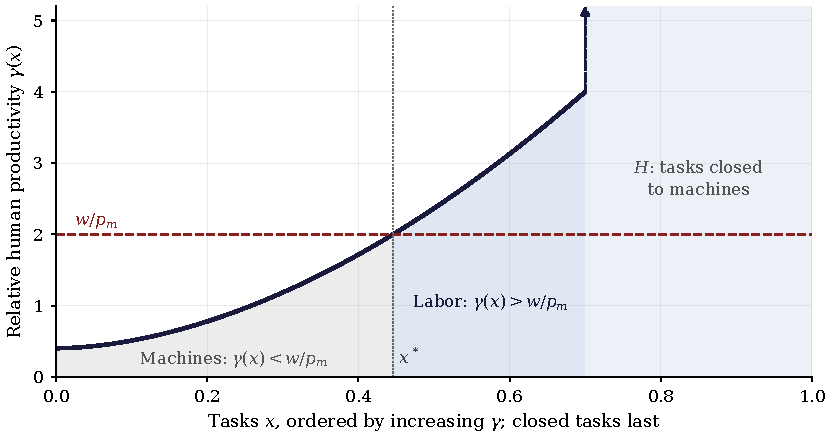
\includegraphics[width=0.88\textwidth]{figures/fig_schedule.pdf}
\caption{The task-assignment schedule. Tasks are ordered so $\gamma(x)$
increases. On the open tasks, the ratio $w/p_m$ divides tasks:
machines hold tasks with $\gamma(x)<w/p_m$, labor holds tasks with
$\gamma(x)>w/p_m$, and an interior margin $x^*$ satisfies equality. Tasks in
$H$ are closed to machines and appear as a wall at the right edge. If labor
holds no open task, the wall marks the boundary assignment in
which wages are determined within the human-required sector. A cheaper machine
or a lower $\gamma$ near an interior margin shifts tasks toward machines. Drawn by code written with Claude (Anthropic).}
\label{fig:1}
\end{figure}

% NEW (design synthesis §3.1), restating main.tex L186-193: (i) adds the boundary and corner inequalities
% (Open 12i); (ii) is main.tex L191 with "movement of the margin" made "movement of an interior margin"
% (design); the authors' (iii) is removed (participation is Proposition 3)
\begin{proposition}[the task margin]\label{prop:1}
In an equilibrium with $w>0$ and $p_m>0$:
(i) at an interior margin,
\[
w=p_m\gamma(x^*);
\]
at a boundary assignment, $w\ge p_m\gamma(x_H)$; at a corner, $w\le p_m\gamma(0)$.
(ii) Holding the machine rental fixed, movement of an interior margin changes the wage at rate $dw/dx^*=p_m\gamma'(x^*)$. Where a fixed-output labor-demand schedule absorbs additional final-task hours by lowering $x^*$, a steeper capability schedule requires a larger wage change for the same movement of the margin.
\end{proposition}

\begin{proof}
% (i) NEW (design synthesis §3.1), replacing main.tex L627's (i), which asserted indifference at every
% boundary between human and machine tasks (Open 12i)
(i) By Definition~\ref{def:equilibrium}(i), $p_m\gamma(x)\le w$ for almost every $x<x^*$ and $p_m\gamma(x)\ge w$ for almost every open task $x>x^*$. At an interior margin both sets have positive measure, and continuity of $\gamma$ at $x^*$ gives equality. At a boundary assignment only the first inequality holds on the open tasks, and at a corner only the second.
% (ii) from main.tex L627, verbatim but for its last sentence, edited: cross-reference (Appendix B's
% complete interior example is now the numerical economy of Section 7); the authors' "(iii) is the
% participation condition." is dropped with Proposition 1(iii)
% Review edit (mathA-4): L627: the symbol N_F, used in the next sentence, is attached to final-task labor demand (it was undefined, as in main.tex)
(ii) Differentiate the equality at fixed $p_m$. If output is $Y$, final-task labor demand is $N_F=Y\int_{x^*}^1dx/\gamma_L(x)$, including the human-required tail. Thus $dN_F/dx^*=-Y/\gamma_L(x^*)$ and $dw/dN_F=-p_m\gamma'(x^*)\gamma_L(x^*)/Y$. Output, the rental, and labor used in machine production also respond in a full equilibrium; Section~\ref{sec:example} supplies a complete interior example under stated conditions.
\end{proof}

% NEW (design synthesis §3.1)
\begin{remark}
Proposition~\ref{prop:1} compares unit costs at given prices. It does not depend on how the machine rental is set, on preferences, or on the labor market.
\end{remark}

% from main.tex L195, verbatim (the loom)
Suppose a loom weaves four meters per hour and a worker weaves one. At $p_m=\$80$ per loom-hour, the two methods have the same weaving cost when the hourly wage is \$20. If the loom improves to five meters per hour, labor's replacement value falls to \$16 at the same rental, with the worker's productivity unchanged. Improvements can differ across weaving, pattern preparation, and repair, changing relative capability unevenly across tasks. This comparison holds the rental and the task fixed; in equilibrium both $p_m$ and the assignment margin may move.

% NEW (build brief §5): Restrepo (2025), one sentence, after Proposition 1; the finding's words are those
% of NBER w34423's abstract (SP/rq/txt/w34423.txt line 53). Then main.tex L229, verbatim
% Review edit (S2): quotation marks: the fourteen words are w34423's abstract, item (iv), verbatim
Restrepo (2025) finds that ``wages converge to the opportunity cost of computational resources required to reproduce human work''.
% from main.tex L229, verbatim
The task margin prices labor against machine services, and the machine-service row prices the substitute against the human hours and non-produced inputs embodied in it.

% NEW (design synthesis §3.1), restating main.tex L231-243: the hypotheses "gamma(x*) > 0, b~_m > 0 and
% 1 - gamma(x*) lambda~_m > 0" become conclusions in the stated economy. Its last sentence is main.tex
% L242, edited: "total requirements" renamed "price coefficients" (Table 1); the design had dropped the
% clause "Holding the other ... fixed", restored here (decision for Stella)
\begin{proposition}[replacement closure]\label{prop:2}
In every equilibrium with an interior margin and $r>0$, the feedback term $1-\gamma(x^*)\widetilde\lambda_m$ is positive and
\begin{equation}\label{eq:5}
\frac{p_m}{r}
=
\frac{\widetilde{b}_m}{1-\gamma(x^*)\widetilde{\lambda}_m},
\qquad
\frac{w}{r}
=
\frac{\gamma(x^*)\widetilde{b}_m}{1-\gamma(x^*)\widetilde{\lambda}_m},
\end{equation}
with $\widetilde\lambda_m$ and $\widetilde b_m$ given by~\eqref{eq:tildem}. Holding the other price coefficients fixed, the wage--rent ratio rises with $\gamma(x^*)$ and with $\widetilde{\lambda}_m$.
\end{proposition}

\begin{proof}
% from main.tex L631-636, edited (design synthesis §3.1): the task condition and the machine-service row
% are named by their new homes, and the design's clause deriving the positivity of the feedback term,
% now a conclusion, is added; the display of the conditional derivatives is verbatim
Substitute $w=p_m\gamma(x^*)$ (Proposition~\ref{prop:1}) into the machine-service row of Lemma~\ref{lem:prices}(i), $p_m=w\widetilde\lambda_m+r\widetilde b_m$, to obtain $p_m(1-\gamma(x^*)\widetilde{\lambda}_m)=r\widetilde{b}_m$. Since $p_m>0$ and $r\widetilde b_m>0$, the feedback term is positive, and solving gives~\eqref{eq:5}. The conditional derivatives are
\[
\frac{\partial(w/r)}{\partial\widetilde{\lambda}_m}=\frac{(\gamma(x^*))^2\widetilde{b}_m}{(1-\gamma(x^*)\widetilde{\lambda}_m)^2},\qquad
\frac{\partial(w/r)}{\partial\gamma(x^*)}=\frac{\widetilde{b}_m}{(1-\gamma(x^*)\widetilde{\lambda}_m)^2},
\]
both positive.
\end{proof}

% NEW (design synthesis §3.1), edited for fix F1: "any production network" becomes "any production network
% of Appendix B.1", since the closure needs Assumption B.1 as F1 restricts it (open tasks an interval)
\begin{remark}
Proposition~\ref{prop:2} uses only Proposition~\ref{prop:1} and the machine-hour's row of the cost system. It does not depend on preferences, on support, or on the labor market, and it holds in any production network of Appendix~\ref{app:networks} whose machine chain uses a non-produced input (Proposition~\ref{prop:network}).
\end{remark}

% from main.tex L245: sentence 1 verbatim; sentences 2-4 as the design restates them (design synthesis
% §3.1, "245, reading on the price basis"): gamma(x*) lambda~_m is labor's share of machine-service cost
% only when rho = 0 (0.567 against 0.456 on the instance), so sentence 2 reads it on the price basis,
% sentence 3's "this share" becomes "it", and sentence 4's "and the selected recipes" (the stated economy
% has one recipe for each good) gives way to a pointer to Theorem 1
The denominator measures the feedback from the wage into the cost of its substitute. At the margin, $\gamma(x^*)\widetilde\lambda_m=w\widetilde\lambda_m/p_m$ is the part of the machine-hour's price that resolves into wages, including the return on the wages advanced to build machines; when $\rho=0$ it is labor's share of machine-service cost. A positive rent bill requires it to be below one. The closure is a price condition at the equilibrium assignment; household choices and market clearing also determine $x^*$ (Theorem~\ref{thm:1}).

% from main.tex L251, edited: cross-reference to Definition 3 added after "either channel", since the
% definitions of the two channels (L249) now stand in Section 3. L251's third sentence ("Actual
% technological changes may alter several coefficients and move the margin together.") is not repeated
% here: the design places it, edited, at the end of Section 3's AI paragraph
Holding the other terms in \eqref{eq:5} fixed, either channel (Definition~\ref{def:automation}) lowers the wage supported by a given rent. With labor in the machine supply chain, task automation also cheapens that chain's labor. Figure~\ref{fig:2} traces both channels from a common starting point.

% from main.tex L253, verbatim (the design's "machine chain" for "full machine-service chain" is not taken)
When the labor requirement of the full machine-service chain vanishes and $\gamma(x^*)\widetilde{\lambda}_m\to0$, equation~\eqref{eq:5} gives
\begin{equation}\label{eq:6}
\frac{p_m/r}{\widetilde{b}_m} \to 1.
\end{equation}
% from main.tex L257, edited: "When $\rho=0$," added to sentence 1 (design synthesis §1.3, "245, 257: When
% rho = 0", and the rho = 0 remark of §3.2: with a positive return, b~_m also carries the return on the
% machines that embody the land); sentence 2 verbatim (the design's rewording of it is not taken)
% Review edit (R18): L257: "two-factor" dropped, the flow benchmark being defined in Section 3.1 (as at L393, D40)
When $\rho=0$, the service price is then accounted for by its embodied claim on the non-produced input. Interest and institutional rents introduce additional income components outside the flow benchmark.

% from main.tex L259-264, verbatim (Figure 2: file and caption unchanged)
\begin{figure}[t]
\centering
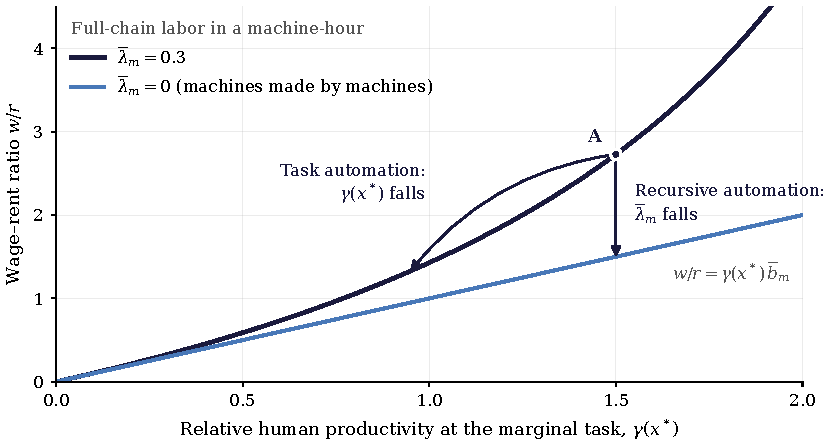
\includegraphics[width=0.88\textwidth]{figures/fig_replacement_closure.pdf}
\caption{The replacement closure \eqref{eq:5}, with $\widetilde{b}_m=1$ and illustrative values. Each curve holds the full-chain labor in a machine-hour, $\widetilde{\lambda}_m$, fixed. The gap between a curve and the line $\widetilde{\lambda}_m=0$ is the feedback from the wage into the cost of its substitute. From A, task automation lowers $\gamma(x^*)$ and moves the economy along its curve; recursive automation lowers $\widetilde{\lambda}_m$ and moves it down to the line, where $w/r=\gamma(x^*)\widetilde{b}_m$. Drawn by code written with Claude (Anthropic).}
\label{fig:2}
\end{figure}

\subsection{Participation and the labor market}\label{sec:participation}

% NEW (design synthesis §3.1), restating main.tex L284-292 with (10) (L304-307) joined to it. "work is
% optimal ... exactly when" is the authors' wording (L285), kept in place of the design's "prefers work
% exactly when", which the math check (C5) found loose at w = s; the last sentence is L291, verbatim
\begin{proposition}[dependence, living costs, and participation]\label{prop:3}
In every equilibrium with $\tau_w=d=g_w=g_e=0$, work is optimal for a worker with cost of work $\chi$ exactly when
\begin{equation}\label{eq:9}
w \ge s,
\qquad
s = (e^{\chi}-1)P_s,
\end{equation}
and employment is
\begin{equation}\label{eq:10}
N_a=NF\left(\log\left[1+\frac{w}{P_s}\right]\right).
\end{equation}
For $\chi>0$, the reservation wage rises with the cost of the basket.
\end{proposition}

\begin{proof}
% from main.tex L640, sentences 1-2, verbatim; then NEW (design synthesis §3.1): the derivative in P_s
% replaces (18), and the tie between work and exit has measure zero
Exit provides utility zero. Work provides $\log(1+w/P_s)-\chi$, which is nonnegative exactly when \eqref{eq:9} holds. For $\chi>0$, $\partial s/\partial P_s=e^\chi-1>0$. Workers with $w=s$ have measure zero because $F$ is continuous, which gives~\eqref{eq:10}.
\end{proof}

% NEW (design synthesis §3.1), edited: the pointer is Appendix D.1 (app:D.1), where the reservation wage
% with payments is derived (main.tex L779-787), in place of the design's pointer to Appendix D as a whole
% Review edit (R23): the NEW pointer is dropped; the authors' paragraph below gives the same pointer
\begin{remark}
Proposition~\ref{prop:3} does not depend on technology, or on who provides the basket, the owner or the government: a worker has one basket in work and in exit either way.
\end{remark}

% from main.tex L294, verbatim
At a fixed wage, a higher basket price reduces the consumption gained from working. With support maintained, participation weakly falls. The condition depends on the wage relative to living costs, so a proportional rescaling of prices leaves the choice unchanged.

% from main.tex L296, edited: cross-reference (Appendix B's fully funded household example is now the
% numerical economy of Section 7, sec:example); app:D.3 and app:D.1 unchanged
% Review edit (R17): L296: "the provider" -> the two agents that can provide support in the rewrite
Maintaining that support requires resources from the owner or the government. Rising housing or care costs can strain a family budget or the capacity of public provision, changing the support available. Section~\ref{sec:example} gives a fully funded household example, and Appendix~\ref{app:D.3} measures how much support rents can finance. Payments that change upon employment are treated in Appendix~\ref{app:D.1}.

% main.tex L268's last sentence (verbatim; the design places it here), then L298 (verbatim), then the
% Korinek and Stiglitz sentence (build brief §5)
% from main.tex L268, last sentence
Access to support, its security, and the obligations it carries help determine the value of exit.
% from main.tex L298
Personal assets, pensions, and savings can also support life outside employment. These sources, together with preferences and the nonpecuniary value of work, influence participation and the prospect of an independent life. The benchmark isolates the choice faced by someone whose living standard is sustained through dependence.
% from main.tex L128, edited: semicolon to period
Korinek and Stiglitz (2019) pose the below-subsistence scenario explored here through dependence and exit.

% from main.tex L300, verbatim (the design's insertion of L124's Lewis sentence is not taken)
Access to common land is a historical example of support through shared resources. Enclosure could remove that access and increase the need for wage income, the mechanism emphasized by Marx (1867), Lewis (1954), and Polanyi (1944). In a modern economy, housing arrangements, household support, and public provision shape the corresponding outside option.

% from main.tex L304, sentence 1, verbatim; then NEW (design synthesis §3.1), restating main.tex L317:
% land is fully used at r > 0 because the owner chooses so (Definition 1(iii)), no longer by assumption
% from main.tex L304, sentence 1
Replacement pricing and participation jointly determine the wage and task assignment.
% NEW (design synthesis §3.1)
If $r>0$, the owner rents out all its land, so by Lemma~\ref{lem:prices}(ii) the economy produces $T/B_s$ baskets and employs $TL_s/B_s$ hours. With Proposition~\ref{prop:3}, labor-market clearing is
% from main.tex L318-321, verbatim
\begin{equation}\label{eq:11}
\underbrace{\frac{TL_s}{B_s}}_{\text{hours required}}
=\underbrace{NF\left(\log\left[1+\frac{w}{P_s}\right]\right)}_{\text{hours supplied}}.
\end{equation}
% from main.tex L322: sentences 1-2 verbatim; sentence 3 edited: cross-references (the household budgets
% now stand in Section 3, and Theorem 1 proves existence and uniqueness); "Appendix B constructs the
% household budgets and proves" becomes "Section 3 constructs the household budgets, and Theorem 1 proves"
The requirements $L_s$ and $B_s$ depend on task assignment. Together with replacement pricing in \eqref{eq:5}, this condition links participation to the equilibrium margin $x^*$. Section~\ref{sec:economy} constructs the household budgets, and Theorem~\ref{thm:1} proves existence and uniqueness under explicit funding conditions.

\subsection{Existence and uniqueness}\label{sec:existence}

% NEW (design synthesis §3.1): main.tex L687's ceiling made a result, with the wall H allowed
\begin{lemma}[the ceiling]\label{lem:ceiling}
Let $x_c$ be the first open task at which $(\rho+\delta)(a+\lambda\gamma(x))\ge1$, or $x_c=x_H$ if there is none. Then $x_c>0$, and in every equilibrium machines perform almost no task in $[x_c,1]$.
\end{lemma}

% NEW (build brief §2, row 4: a remark after each result), modeled on Proposition 1's; "at the user cost"
% for fix F5
\begin{remark}
Lemma~\ref{lem:ceiling} compares unit costs at the user cost. It does not depend on preferences or on the labor market.
\end{remark}

% NEW (design synthesis §3.1), restating main.tex L687, sentences 1-2, without calling the ceiling
% "closed" (closure is now H's, by capability or by rule)
% Review edit (R3-1): H includes tasks reserved by rule, which machines could perform (Assumption 1)
Machines do not perform the tasks in $H$, which are closed to them by capability or by rule. At a task in $[x_c,x_H]$ they can, but the machine-hours that would replace an hour there embody at least that hour of labor, counting the labor needed to build them at the required return, so they cost at least the hour at any wage. Unlike $H$, the ceiling depends on the labor in the machine chain and on the return, as well as on capability.

% from main.tex L687, sentences 3-4, and L688-697 ((21), its lead-in and (22)), verbatim
At an interior threshold $x<x_c$, machines perform tasks below $x$ and people those above it. The task condition and the user cost give
\begin{equation}\label{eq:21}
J(x)=\int_0^x\gamma(t)\,dt,\qquad
p_m(x)=\frac{(\rho+\delta)b}{1-(\rho+\delta)(a+\lambda\gamma(x))},\qquad
v(x)=\gamma(x)\,p_m(x).
\end{equation}
The final-good and basket prices are
\begin{equation}\label{eq:22}
p(x)=v(x)(1-x)+p_m(x)J(x),\qquad
P_s(x)=p(x)+h.
\end{equation}
% from main.tex L698-702, verbatim
If final-good output is $Y$, total consumption contains $Y$ baskets and uses $hY$ units of space. In a stationary state a machine stock $X$ supplies $X$ units of service: $YJ(x)$ to final tasks and $a\delta X$ to rebuilding the $\delta X$ machines that wear out each period. Machine and land clearing give
\begin{equation}\label{eq:23}
Y(x)=\frac{T}{h+b\delta J(x)/(1-a\delta)},\qquad
X(x)=\frac{Y(x)J(x)}{1-a\delta}.
\end{equation}
% from main.tex L703-707, edited: n_D and n_S renamed N_D and N_S (Table 1)
Labor demand and supply are
\begin{equation}\label{eq:24}
N_D(x)=Y(x)\left[1-x+\frac{\lambda\delta J(x)}{1-a\delta}\right],\qquad
N_S(x)=NF\left(\log\left[1+\frac{v(x)}{P_s(x)}\right]\right).
\end{equation}
% from main.tex L708: sentence 1 verbatim; then NEW (design synthesis §3.1, its note replacing L708's limit
% sentence): N_S(x_c) is defined as the limit of the margin-indexed supply (the math check C4 requires this
% reading of (25)), and the unbounded case is stated for a ceiling below the wall
The two components of demand are final-task and machine-sector hours. As $x$ rises to $x_c$, $N_S(x)$ tends to a limit, which we write $N_S(x_c)$. If the ceiling binds before $H$, $v$ and $P_s$ grow without bound while $v/P_s$ tends to $\gamma(x_c)/[\gamma(x_c)(1-x_c)+J(x_c)]$.

% NEW (design synthesis §3.1), restating main.tex L719-726 (Lemma B.1): every equilibrium is the interior
% one, and funding is necessary as well as sufficient (Open 12(h)). With fix F5 the weak inequality stays:
% Definition 1 allows c_o = 0
% Review edit (D25): "and of workers" added: workers indifferent between work and exit have measure zero (math check C4, condition 3)
\begin{theorem}[existence and uniqueness]\label{thm:1}
With every instrument zero and the owner providing support, suppose
\begin{equation}\label{eq:25}
T>Nh,\qquad
N_S(x_c)>N_D(x_c).
\end{equation}
Then every equilibrium has $w>0$, $r>0$, and an interior margin, at the unique $x^*\in(0,x_c)$ with $N_D(x^*)=N_S(x^*)$. Up to the choice of numeraire and sets of tasks and of workers of measure zero, its prices are \eqref{eq:21}--\eqref{eq:22} and its quantities \eqref{eq:23}--\eqref{eq:24} at $x^*$. An equilibrium exists if and only if the owner's income covers the support there, $rT+\rho V_mX\ge NP_s$.
\end{theorem}

% NEW (design synthesis §3.1), edited for fix F5: "and the user cost" added, since the proof excludes a
% zero rent (and every return other than rho) through the user-cost clause of Definition 1(i)
The proof (Appendix~\ref{app:proofs}) uses~\eqref{eq:25} and the user cost to rule out a zero wage, a zero rent, a corner, a margin at the ceiling, and a boundary assignment at the wall; one crossing remains, and the owner's budget decides whether it is an equilibrium.

% NEW (design synthesis §3.1), with fix F5: the second and third sentences are new. The third is F5's
% plain sentence; the design's claim that the user-cost clause "costs nothing" (synthesis.md 584-587,
% 1183) is not carried into the text
% Review edit (D30): F5's plain sentence is dropped from this remark; it prints after Definition 1 and, with its reason, in the remark after Lemma A.1
\begin{remark}
Theorem~\ref{thm:1} does not depend on the shape of $\gamma$ beyond Assumption~\ref{ass:tasks}, or on whether $H$ is empty, once~\eqref{eq:25} holds. Its uniqueness rests on the clause of Definition~\ref{def:equilibrium}(i) that machine-hours rent at the user cost. When the wall lies below the crossing, \eqref{eq:25} fails: labor demand still exceeds supply at $x_H$, no interior margin clears the labor market, and labor works only in $H$ and in the machine chain. The theorem does not cover that case.
\end{remark}

% NEW (design synthesis §3.1): (i) collects main.tex L324 (sentence 1) and L729-734 and adds the
% equilibrium rate; (ii) restates main.tex L743 (and L324, sentence 2)
\begin{corollary}[labor supply and the margin]\label{cor:statics}
(i) As the margin $x$ rises on $(0,x_c)$, labor demand $N_D(x)$ falls, while the wage--rent ratio $v(x)$ and the real wage $v(x)/P_s(x)$ rise; the wage--rent ratio rises at the rate $dv/dx=p_m\gamma'(x)/[r(1-\gamma(x)\widetilde\lambda_m)]$, the rate of Proposition~\ref{prop:1}(ii) amplified by $1/(1-\gamma\widetilde\lambda_m)=1+\lambda v/b$ because the machine rental rises with the margin.
(ii) If the distribution of work costs changes from $F$ to $\widehat F\le F$ at fixed technology and support, and \eqref{eq:25} and funding hold under both, the equilibrium margin, wage--rent ratio, and real wage weakly rise, and strictly if supply falls at the original margin.
\end{corollary}

% NEW (design synthesis §3.1)
\begin{remark}
Part~(i) concerns the margin-indexed functions \eqref{eq:21}--\eqref{eq:24} and does not need~\eqref{eq:25}; part~(ii) does not depend on the form of $F$.
\end{remark}

% ---- build part 05_purchasing.tex (SP/build/parts/05_purchasing.tex) ----
% ============================================================
% Section 5: Purchasing power and income (BRIEF section 2, row 5).
% Built from main.tex L88 (moved verbatim to open the section); design synthesis.md section 3.2; main.tex L90
% (sentence 1), L128 (the Caselli and Manning sentence), L132 (the factor-share clause), L334, L351, L353, L374, L376
% and L393; fixes F2 and F3 (BRIEF section 4). The proofs of Proposition 4, Corollary 2 and Proposition 5 are in
% Appendix A (app:proofs). Notes: parts/05_06.notes.md.
% ============================================================
\section{Purchasing power and income}\label{sec:purchasing}

% from main.tex L88 (moved here from the introduction)
At an interior task margin, the wage relative to rent links automation to purchasing power. Holding the selected input requirements fixed, a fall in relative human productivity at the margin lowers the wage relative to rent; reducing the labor embodied in machine services lowers it further. Every good's price resolves into its direct and indirect labor and non-produced input requirements. The embodied rent bill places an upper bound on what an hour's wage can buy. A feasible human production method supplies a complementary lower bound through its labor cost and rent bill. If the wage--rent ratio tends to zero, wage purchasing power tends to zero for goods whose embodied requirement for the non-produced input stays bounded away from zero. A feasible method requiring bounded human hours and no non-produced input anywhere in its chain preserves a positive lower bound.

\subsection{What an hour's wage buys}\label{sec:wagebuys}

% from main.tex L334 (sentences 1-2), edited: "the total requirements" -> "the price coefficients" (the design's Table 1
% name for the tilde coefficients of eq. (4), which with durable machines are valued at the user cost)
For every good or service, the price coefficients in~\eqref{eq:4} give an exact price. A feasible alternative method also bounds that price from above.
% NEW (design synthesis §3.2)
A worker can make a unit of the final good by hand in an hour, using neither machines nor land.

% NEW (design synthesis §3.2): Proposition 4 restated in the stated economy; replaces main.tex L336-349. The general
% bounds of L343-347 are eq. (13) in the remark below and Proposition B.1(c).
\begin{proposition}[the real-wage fork]\label{prop:4}
In every equilibrium with $w,r>0$, every good or service $i$ satisfies
\begin{equation}\label{eq:12}
p_i=w\widetilde\lambda_i+r\widetilde b_i,\qquad
\frac{w}{p_i}=\frac{1}{\widetilde\lambda_i+\widetilde b_i(r/w)}.
\end{equation}
An hour's wage buys $w/r$ units of space and at least one unit of the final good; when machines perform some tasks, it buys at most $(w/r)/\widetilde b_g$ units of the final good, where $\widetilde b_g=\widetilde b_mJ(x^*)>0$.
\end{proposition}

% from main.tex L90 (sentence 1), edited: "Acemoglu and Restrepo" -> "Acemoglu and Restrepo (2018)" (citation year; the
% references hold their 2018, 2022 and 2026 papers). Moved from the introduction to stand directly after Proposition 4.
Combining the task margin of Acemoglu and Restrepo (2018) with the input--output price logic of Leontief (1936) and Sraffa (1960) yields these purchasing-power bounds.
% from main.tex L128 (the Caselli and Manning sentence), edited: "Section~\ref{sec:6}" -> "Proposition~\ref{prop:4}"
% (the section pointer; the lower bound is now Proposition 4's, stated just above). BRIEF section 5.
Caselli and Manning (2019) prove that real wages cannot fall in terms of goods produced entirely from reproducible inputs; Proposition~\ref{prop:4} gives a lower bound from feasible human production and shows how persistent requirements for non-produced inputs constrain wage purchasing power.

% NEW (design synthesis §3.2): the remark on what Proposition 4 does not depend on. Eq. (13) is main.tex L343-347 with
% \bar L_i renamed \bar\lambda_i (design synthesis §2.3), on the human chain of Appendix B.1.
% Review edit (R20): the subscript h, defined only in Appendix B.1, is dropped
\begin{remark}
Proposition~\ref{prop:4} does not depend on the margin being interior, or on there being four goods. In any production network, every good $i$ that people can make with a \emph{human chain}, which uses neither machines nor machine-hours anywhere and has full-chain requirements $\bar\lambda_i$ of hours and $\bar b_i$ of non-produced services, satisfies
\begin{equation}\label{eq:13}
\frac{1}{\bar\lambda_i+\bar b_i(r/w)}
\le\frac{w}{p_i}
\le\frac{w/r}{\widetilde b_i}
\end{equation}
when $\widetilde b_i>0$ (Proposition~\ref{prop:network}). Here the final good has $\bar\lambda=1$ and $\bar b=0$, and space, which rents at $r$, has $\widetilde b=1$.
\end{remark}

% from main.tex L351, edited: (a) sentence 2 is read on the price basis (design synthesis §3.2: with durable machines
% \widetilde b_i is a price coefficient, at least the input the unit embodies and equal to it when rho = 0); it was
% "An hour's wage buys $w/r$ units of the non-produced service; a unit of output embodies $\widetilde b_i$ units."
% (b) last sentence: "Appendix~\ref{app:A.3}" -> "Appendix~\ref{app:extensions}" (task-level costs are now Appendix B.6).
% assembly (label fix): app:extensions -> app:tasklevel, Appendix B -> Appendix B.6; narrowed to B.6 (task-level costs), the label part 12 defines; part 05 notes: the pointer can be narrowed if B.6 gets a label; part 12 notes (f)
The rent bound counts the whole supply chain. An hour's wage buys $w/r$ units of the non-produced service, and the price of a unit of output carries $\widetilde b_i$ units, the return on the machines in its chain included; when $\rho=0$, $\widetilde b_i$ is the input the unit embodies. A good with no direct requirement may still use that input through electricity, materials, or machinery. The human-method bound likewise counts its entire chain. For cloth, consider a feasible hand-production method covering the fibers, spinning, weaving, tools, and workspace. The wage and rent bill for that complete chain caps the competitive price of cloth. Cheaper machine production raises what an hour's wage can buy above the lower bound. Ownership income and transfers fund consumption in addition to wages. Appendix~\ref{app:tasklevel} gives the task-level representation of these costs.

% from main.tex L353, edited: (a) ", valued at the user cost" added after "throughout those supply chains" (design
% synthesis §3.2, the price basis); (b) $\bar L_i$ -> $\bar\lambda_i$ (design synthesis §2.3, to match eq. (13) above)
% Review edit (R08): L351: "total human requirements" (a name the rewrite no longer defines) -> the symbol
Changes in purchasing power depend jointly on the wage--rent ratio and the requirements embodied in each good. Building taller can supply more floor space on a given site, lowering direct site area per unit. Higher crop yields can reduce the acreage needed for a given number of calories. These changes also alter requirements for structures, machinery, fertilizer, and energy; $\widetilde b_i$ counts the non-produced inputs throughout those supply chains, valued at the user cost. At given wages, rents, and $\widetilde\lambda_i$, a lower $\widetilde b_i$ reduces the price. Equilibrium affordability also depends on the wage--rent ratio. The ratio $\bar b_i/\bar\lambda_i$ describes how strongly rents enter the human-method lower bound; ordering actual price changes requires the selected recipes.

% NEW (design synthesis §3.2): Corollary 2 restated; replaces main.tex L355-368 (its proof, L370-372, is in Appendix A).
% Fix F2 keeps the drafted hypotheses ("F fixed" and g_w <= g_e) and claims neither is necessary.
\begin{corollary}[vanishing wage purchasing power and participation]\label{cor:vanishing}
Along a sequence of equilibria with interior margins and a fixed $h$, suppose
\[
\gamma(x^*)\widetilde b_m\to0,\qquad
1-\gamma(x^*)\widetilde\lambda_m\ge\xi>0.
\]
Then $w/r\to0$: an hour's wage buys ever less space, while it still buys at least one unit of the final good. If, in addition, the distribution $F$ of work costs is fixed and no public payment favors work, $g_w\le g_e$, then
\begin{equation}\label{eq:14}
\frac{w}{P_s}\to0,\qquad
\frac{N_a}{N}\to0.
\end{equation}
\end{corollary}

% NEW (design synthesis §3.2). Its last sentence is NEW, for fix F2 (BRIEF section 4; verdicts C2): synthesis.md
% line 1259's bound F(log(1+theta)) holds only when d = g_e = 0, so the general bound is given, and with it the case
% d = g_e = 0. Algebra checked in work/05_06/check_numbers.py.
\begin{remark}
Corollary~\ref{cor:vanishing} does not depend on which channel drives $\gamma(x^*)\widetilde b_m$ to zero. Recursive automation alone cannot: with no labor in the machine chain, $w/r=\gamma(x^*)\widetilde b_m>0$, so people leave work only as machines improve at the tasks people still do. In a production network the corollary holds good by good, for every good whose price coefficient $\widetilde b_i$ stays bounded away from zero (Proposition~\ref{prop:network}). Without the condition $g_w\le g_e$, a payment can keep people working: if $g_w=g_e+\theta P_s$ with $\theta>0$, every worker with $\chi\le\log[1+\theta P_s/(P_s+d+g_e)]$ works at any wage, so $N_a/N\ge F(\log[1+\theta P_s/(P_s+d+g_e)])$, which is $F(\log(1+\theta))$ when $d=g_e=0$.
\end{remark}

% from main.tex L374, edited: "Appendix~\ref{app:B}" -> "Section~\ref{sec:example}" (the numerical economy and its
% path are now Section 7). The "hundred-to-one" anchor of checks/check_interior.py is kept.
The conditions concern replacement at the equilibrium margin. At fixed positive $\gamma(x^*)$ and $\widetilde b_m$, eliminating embodied labor from machine services leaves $w/r=\gamma(x^*)\widetilde b_m>0$. Human-required work can sustain a boundary assignment, and falling non-produced input requirements can sustain purchasing power. Section~\ref{sec:example} gives a complete interior equilibrium and a sequence with a persistent hundred-to-one capability ratio across tasks.

% from main.tex L376, edited: "Section~\ref{sec:7}" -> "Section~\ref{sec:rent}" (cross-reference)
The participation conclusion depends on maintaining the outside option. As wages buy less additional consumption, fewer people choose work when their basic support remains available. If providers' resources shrink and support falls, the participation response can change. Section~\ref{sec:rent} connects the funded basket to the income available for redistribution.

% from main.tex L378 (the subsection title, kept; the design shortens it to "Factor income")
\subsection{Factor income while labor remains employed}\label{sec:income}

% NEW (design synthesis §3.2): Proposition 5 restated with the return on machines; replaces main.tex L380-387 (its
% proof, L389-391, is in Appendix A). Fix F3 (BRIEF section 4; verdicts C3): equality if rho = 0 and, when N_a > 0,
% only then (with r > 0, w, V_m and X are positive in every equilibrium, so rho V_m X = 0 exactly when rho = 0).
% The last two sentences are main.tex L386: the first, "At given $N_a$ and $T$, a lower wage--rent ratio lowers labor's
% share.", edited: prefixed "When $\rho=0$," (it needs rho = 0); the second verbatim.
\begin{proposition}[labor's share]\label{prop:5}
In every equilibrium, final expenditure equals factor income,
\begin{equation}\label{eq:income}
I=wN_a+rT+\rho V_mX,
\end{equation}
where $N_a$ counts all employed hours, including those in machine production, and $\rho V_mX$ is the return on the machine stock. If $r>0$, labor's share satisfies
\begin{equation}\label{eq:15}
\frac{wN_a}{I}\le\frac{(w/r)N_a}{(w/r)N_a+T},
\end{equation}
with equality if $\rho=0$ and, when $N_a>0$, only if $\rho=0$. When $\rho=0$, at given $N_a$ and $T$, a lower wage--rent ratio lowers labor's share. With bounded total hours and fixed $T>0$, $w/r\to0$ implies that labor's share tends to zero.
\end{proposition}

% NEW (design synthesis §3.2); its first clause is main.tex L757's last sentence made a remark. The design's stray
% source marker "(757)" is moved into this comment.
\begin{remark}
The identity does not depend on which cost-minimizing assignment supplies the coefficients, and it holds in any production network (Proposition~\ref{prop:network}).
\end{remark}

% from main.tex L393 (sentence 1), edited: "in this two-factor flow benchmark" -> "When $\rho=0$," at the front (the
% design's "when rho = 0" in place of "in the flow benchmark", exact for every delta), and the design's clause on the
% return on machines added (synthesis §3.2); old: "Ownership of the non-produced input receives the non-wage component
% of income in this two-factor flow benchmark."
When $\rho=0$, ownership of the non-produced input receives the non-wage component of income; with a positive return the owner also receives the return on machines, which~\eqref{eq:income} counts.
% NEW (design synthesis §3.2); numbers from code/appendix_b.py (wages 0.5505, rent 0.1277, interest 0.3218 of income;
% bound 0.8117), reproduced in work/05_06/check_numbers.py
In the instance of Section~\ref{sec:example}, income is $0.55$ wages, $0.13$ rent, and $0.32$ return on machines, and labor's share is $0.55$ against the $0.81$ that~\eqref{eq:15} gives as its bound.
% from main.tex L393 (sentences 2-5), edited: sentence 3's "this benchmark" -> "the flow benchmark" (its antecedent,
% sentence 1's "this two-factor flow benchmark", is gone; interest is inside the stated economy, outside the flow
% benchmark)
% Review edit (mathB-3): L393: "funded-support" dropped; Corollary 2 no longer has a funding hypothesis (funding is in Definition 1)
The wage bill includes work throughout the network; eliminating labor from machine services leaves any human hours used elsewhere in the income identity. Interest, institutional rents, and transitional capacity rents add income components outside the flow benchmark. Labor's share responds jointly to the wage--rent ratio and employment, so increased employment can offset a local fall in $w/r$. When the conditions for \eqref{eq:14} also hold, both the wage--rent ratio and the employed fraction tend to zero.
% from main.tex L132 (Section 2.7's factor-share clause), edited: "Factor shares:" -> "In the data," to open a sentence
% (design synthesis §3.2) and "Piketty and Zucman 2014" dropped (BRIEF section 5); the authors' "---" is kept
In the data, the labor share's decline is documented and global (Karabarbounis and Neiman 2014), and its capital-side counterpart resolves substantially into housing --- which is to say land (Rognlie 2015; Knoll, Schularick, and Steger 2017).

% NEW (design synthesis §3.2, the rho = 0 remark), with fix F3: "\eqref{eq:15} holds with equality only then" ->
% "when $N_a>0$, \eqref{eq:15} holds with equality only then" (verdicts C3: when nobody works both sides are zero)
Durable machines change five statements, each of which holds as in the flow benchmark when $\rho=0$, whatever $\delta$: the basket's price equals $wL_s+rB_s$ only when $\rho=0$, and otherwise also pays the return on the machines that supply it; when $N_a>0$, \eqref{eq:15} holds with equality only then; Proposition~\ref{prop:6}(iii) and Corollary~\ref{cor:fiscal} count the return on machines beside rent; \eqref{eq:17} is equivalent to physical feasibility only then; and the readings of $\gamma(x^*)\widetilde\lambda_m$, of~\eqref{eq:6}, and of $\widetilde b_i$ as physical quantities need it. Every other statement holds as stated with durable machines.

% ---- build part 06_rent.tex (SP/build/parts/06_rent.tex) ----
% ============================================================
% Section 6: Distribution: rent taxation and a uniform transfer (BRIEF section 2, row 6).
% Built from main.tex L397, L223-225 (all but its first sentence, which Section 3 keeps), L402-410, L417-425, L437-439
% and L268's fifth sentence (placed at L437, as the design maps it); design synthesis.md section 3.3 (Proposition 6
% and its remark, (16) with public provision, the funding paragraph, Corollary 3 and its remark); fix F6 (BRIEF
% section 4); the lilies aside (BRIEF section 6); Korinek and Lockwood (2026) beside George (1879) (BRIEF section 5).
% The proofs of Proposition 6 (main.tex L413-415) and Corollary 3 (main.tex L769-775) are in Appendix A (app:proofs).
% Notes: parts/05_06.notes.md.
% ============================================================
\section{Distribution: rent taxation and a uniform transfer}\label{sec:rent}

% from main.tex L397
The income identity separates two sources of purchasing power: hours sold and ownership claims. A lower wage--rent ratio increases the importance of ownership at given employment. Rent taxation and transfers determine how this income is distributed across households.

% from main.tex L223-225 (sentences 2-7; sentence 1, on the cost recursion, is in Section 3), edited: sentence 6's
% "Appendix~\ref{app:A}" -> "Appendix~\ref{app:extensions}" (several non-produced inputs are now Appendix B.2). The design
% moves the definitions here, where the tax uses them (synthesis §1.3 and §3.3); it shows only sentences 2 and 5.
An input is \emph{terminal over a horizon} when its supply cannot expand through production within that horizon. Land is a lasting example; installed grid connections or fabrication capacity may be terminal temporarily. Electricity, structures, and extraction are activities whose input costs are traced through the system. We reserve \emph{pure rent}
for income due to fixed supply and \emph{site rent} for the land component of
% assembly (label fix): app:extensions -> app:inputs, Appendix B -> Appendix B.2; narrowed to B.2 (several non-produced inputs), the label part 12 defines; part 12 notes (f)
real-estate income, excluding structures. Several non-produced inputs enter as $\mathbf{B}\mathbf{r}$ in Appendix~\ref{app:inputs}. Long-run applications require persistent non-produced inputs.

% NEW (design synthesis §3.3): Proposition 6 with its instruments named; replaces main.tex L399 and restates L401-411.
% (i) opens with a NEW sentence, the owner's choice under the rental-value tax (Lemma A.1(a)), then main.tex L402's two
% sentences verbatim. (ii) is main.tex L404 verbatim. (iii) is main.tex L406-410, edited: "remain $wN_a+R$" -> "remain
% $wN_a+R+\rho V_mX$" (the return on machines); its last sentence keeps the authors' "per-person" (the design wrote
% "per-worker"; Section 3 states that "per person" means per worker).
% Review edit (mathB-4): R is defined where it is first used (it was defined only in the coverage paragraph after Proposition 6's remark)
\begin{proposition}[sharing rents while labor remains employed]\label{prop:6}
Let the government tax the rental value of land, $R=rT$, at $\tau_R\in[0,1]$ and pay $d=\tau_RR/N$ to every worker, with $\tau_w=g_w=g_e=0$ and $\sigma=1$.

(i) At any positive rent the owner rents out all its land, whatever the tax rate. The physical supply of the fixed factor is invariant to a tax on its pure ownership rent. Producers continue to pay the gross competitive rental for using it.

(ii) An unconditional transfer pays the same amount in work and exit. Its direct payment differential at the participation boundary is zero, while participation can respond through income effects.

(iii) At given gross prices and hours, aggregate receipts remain $wN_a+R+\rho V_mX$, since
\[
(1-\tau_R)R+Nd=R.
\]
The tax redistributes the rent component toward an equal per-person allocation.
\end{proposition}

% NEW (design synthesis §3.3)
\begin{remark}
Proposition~\ref{prop:6} does not depend on demand or supply elasticities: the taxed input's supply is fixed, and the tax does not depend on its use. With a tax on rent received instead, part~(i) would hold only for $\tau_R<1$.
\end{remark}

% from main.tex L417-421, edited for public provision (design synthesis §3.3; BRIEF row 6, "(16) with public
% provision"): sentence 2's "with $R>0$" -> "with $R=rT>0$" (Table 1's R; L399, which defined R, is replaced by
% Proposition 6); sentence 3's "Funding exactly one basket per person requires $d=P_s$, hence" -> "If the government
% provides the basket ($\sigma=0$) from the rent tax alone, its budget~\eqref{eq:govbudget} requires". Sentences 1, 4
% and 5 verbatim (the design rewrote sentence 1 and cut sentence 5; neither change is taken).
Rent revenue can finance the basket underlying the participation choice. Define coverage by $\kappa=R/(NP_s)$, with $R=rT>0$. If the government provides the basket ($\sigma=0$) from the rent tax alone, its budget~\eqref{eq:govbudget} requires
\begin{equation}\label{eq:16}
\tau_R=\frac{NP_s}{R}=\frac{1}{\kappa}.
\end{equation}
A tax rate between zero and one can meet this budget exactly when $\kappa\ge1$, evaluated at equilibrium prices. Appendix~\ref{app:D.3} relates coverage to the basket's input requirements.

% from main.tex L423, edited: "Section~\ref{sec:4}'s preferences" -> "Section~\ref{sec:workers}'s preferences"
% (cross-reference). The design's rewording of sentences 1-2 and its cut of sentences 3-4 are not taken: each holds as
% written in the stated economy (sentence 1 is public provision, sigma = 0, at unchanged prices; sentence 2 is a
% transfer on top of the owner's basket, sigma = 1 and d > 0).
Replacing existing household or public financing while maintaining total support and prices leaves the participation comparison unchanged. If the payment supplements the existing basket, Section~\ref{sec:workers}'s preferences instead give the reservation wage $(e^\chi-1)(P_s+d)$: the extra consumption available in both states reduces the gain from work. Redistribution can also change demand, rents, and the resources of support providers. These equilibrium effects determine whether the promised basket remains funded.

% NEW (design synthesis §3.3): what funded support requires at rho = 0, and how the measured coverage fits. Numbers:
% kappa = 0.30 is main.tex L494; rent covers 0.3848 of support in the instance (code/appendix_b.py, reproduced in
% work/05_06/check_numbers.py; the return on machines covers 0.9696 of it).
With every instrument at zero, the owner's budget~\eqref{eq:ownerbudget} requires $rT+\rho V_mX\ge NP_s$, so at $\rho=0$ every equilibrium has $\kappa\ge1$. The measured coverage, $0.30$ (Section~\ref{sec:measurement}), therefore fits the stated economy only with another source of support: in the instance of Section~\ref{sec:example}, rent covers $0.38$ of it and the return on machines the rest.

% from main.tex L425
A wage-funded transfer draws on the labor market as both a financing base and a participation margin. Its incidence depends on demand and supply elasticities. The limiting case also constrains how much support that base can finance.

% NEW (design synthesis §3.3): Corollary 3 restated; replaces main.tex L427-435 (its proof is in Appendix A).
% (i) is main.tex L428, edited: "while $R/I\to1$" -> "while the non-wage share of income, $(R+\rho V_mX)/I$, tends to
% one; when $\rho=0$, $R/I\to1$" (the design's change: R/I need not tend to one when rho > 0); otherwise verbatim, so the
% design's rewording of the rest of (i) is not taken. (ii)'s first sentence is the design's (a statement about prices at
% given methods, with (17) on the price coefficients), replacing L430-433. Its second sentence is main.tex L434,
% edited: "exactly when $NB_s\le T$, the physical feasibility condition" -> "exactly when $N\widetilde b_s\le T$, which
% implies $NB_s\le T$, the physical feasibility condition", and the design's closing clause added ("when $\rho=0$, ...
% coincide"), in place of the design's rewording of L434.
\begin{corollary}[fiscal capacity as wage income vanishes]\label{cor:fiscal}
(i) In the one-input economy, let $N,T>0$ be fixed and $N_a\le N$. Along a sequence of equilibria with $w/r\to0$, revenue from any wage tax with a rate between zero and one becomes a vanishing fraction of total income, while the non-wage share of income, $(R+\rho V_mX)/I$, tends to one; when $\rho=0$, $R/I\to1$. If the basket's total non-produced input requirement $B_s$ stays bounded away from zero, that revenue also funds a vanishing fraction of one basket per person.

(ii) At given methods that use no labor anywhere in the basket's chain, $\widetilde\lambda_s=0$, and any rent $r>0$, full rent capture yields coverage
\begin{equation}\label{eq:17}
\kappa=\frac{T}{N\widetilde b_s}.
\end{equation}
It funds one basket per person exactly when $N\widetilde b_s\le T$, which implies $NB_s\le T$, the physical feasibility condition for the basket under these recipes; when $\rho=0$, $\widetilde b_s=B_s$ and the two conditions coincide.
\end{corollary}

% NEW (design synthesis §3.3), with two edits for rule 2 of the brief (no "not X but Y" contrasts in new prose): "Part
% (ii) is a statement about prices at given methods, not about an equilibrium: ..." -> "... at given methods: ..., so
% such a configuration is not an equilibrium"; "which compares rental values rather than physical quantities" ->
% "which compares rental values". The last two sentences are NEW, fix F6 (BRIEF section 4; STATE 2026-11-05, "Eq. (17)
% is narrower than the question it would answer"): the several-input line, checked against the several-input cost
% system of Appendix B.2 (main.tex L576-588, L594) and on 3,692 random networks in work/05_06/check_numbers.py; and the
% durable line, from intro/verify_claims/durable_coverage.py (1.707153 and 0.659369 at N = 1).
\begin{remark}
% assembly (label fix): app:extensions -> app:inputs, Appendix B -> Appendix B.2; narrowed to B.2 (several non-produced inputs), the label part 12 defines; part 12 notes (f)
% Review edit (V2): the claim holds when no payment favors exit; with g_e > g_w + (1 - tau_w)w nobody works at that wage
Part~(ii) is a statement about prices at given methods: with $H$ empty, a configuration with no labor in the basket's chain demands no labor, while, if no payment favors exit ($g_e\le g_w$), every positive wage draws some workers when $F(z)>0$ for $z>0$, as in the instance, so such a configuration is not an equilibrium. With several non-produced inputs, \eqref{eq:17} becomes $\kappa=\mathbf r^{\top}\mathbf T/(N\mathbf r^{\top}\widetilde{\mathbf b}_s)$, which compares rental values (Appendix~\ref{app:inputs}). When $\rho=0$ and every input that earns a positive rent is fully used, rent equals the value of the baskets produced, whose number the scarcest input limits, so the condition holds input by input: full capture funds one basket per person exactly when $NB_{s,k}\le T_k$ for every input $k$, where $B_{s,k}$ is the amount of input $k$ that one basket physically requires. With durable machines, rent and interest together fund the basket, since without labor they make up all income: at the parameters of the instance in Section~\ref{sec:example}, with $\lambda=0$ and machines performing every task, full capture of rent and interest funds $1.71$ baskets per person, and rent alone funds $0.66$.
\end{remark}

% NEW (BRIEF section 6: the aside, exact text, decided by Stella; STATE 2026-11-05). Keynes's words checked against
% rq/keynes.txt: "the lilies of the field who toil not, neither do they spin"; "honoring" is the paper's spelling.
Keynes (1930) looked forward to honoring ``the lilies of the field who toil not, neither do they spin.'' Equation~\eqref{eq:17} adds two conditions: the field must be large enough, and its rent must reach the lilies.

% from main.tex L437 (sentence 1)
As the wage--rent ratio tends to zero, maintaining access to a living basket with a persistent non-produced input requirement increasingly depends on ownership income or transfers.
% from main.tex L268 (sentence 5), edited: "(Section~\ref{sec:owner})" added, a cross-reference to the parents' example
% that the sentence continues (now in Section 3). The design moves this sentence here (synthesis §1.3, "268's sentence
% on wage-financed parents moves to §5 (437)"), and part 04 lists it as placed here.
% Review edit (V1): the pointer follows the parents example to Section 2, where it now prints alone (D6)
The parents (Section~\ref{sec:description}) may themselves finance that support from wages.
% from main.tex L437 (sentences 2-6)
Support financed by another household member's wage faces the same aggregate constraint. A system funded entirely from wages becomes unable to sustain a fixed positive basket entitlement for everyone sufficiently far along the path, while labor may still be employed. A uniform rent dividend gives each person a claim on the income that remains. Broad ownership, collective funds, and other transfer arrangements can also distribute those claims. The financing constraint establishes the need for income beyond wages; institutions determine its distribution and the pace of adjustment.

% from main.tex L439, edited: "Appendix~\ref{app:D} proves the corollary and develops" -> "Appendix~\ref{app:proofs}
% proves the corollary, and Appendices~\ref{app:D.2} and~\ref{app:D.3} develop" (cross-references: the proof is now in
% Appendix A, design synthesis §1.3 "The pointer becomes Appendix A"; incidence and coverage stay in D.2 and D.3, whose
% labels the brief keeps, while Appendix D's own label may be app:D or the design's app:fiscal)
Appendix~\ref{app:proofs} proves the corollary, and Appendices~\ref{app:D.2} and~\ref{app:D.3} develop payroll-tax incidence and rent-base coverage while labor remains employed. The fiscal lineage is George (1879); the Henry George theorem of Arnott and Stiglitz (1979) is related but distinct.
% NEW (BRIEF section 5: one sentence beside George (1879), as given). Korinek and Lockwood (2026), NBER w34873, Section
% 3.4 and its Proposition 5, in an extension with reproducible capital, a fixed factor and no labor: "taxing fixed
% factors is non-distortionary and can achieve powerful redistribution" (rq/txt/w34873.txt).
Korinek and Lockwood (2026) show that in an economy without labor, taxing fixed factors is non-distortionary and can redistribute.

% ---- build part 07_example.tex (SP/build/parts/07_example.tex) ----
% =====================================================================================================
% Section 7. A numerical economy and an automation path (sec:example). Build part 07, 2026-11-05.
% Built from design synthesis §3.4 (Table 2, the instance, Figure 3 with the artificial-intelligence
% framing in the text, the path) and the authors' text wherever its content carries over: main.tex L745
% (the instance), L310-315 (Figure 3, moved here from Section 5), L324, sentences 3-7 (sentences 1-2 are
% Corollary 1 in Section 4, part 04), and L747 (the path). The design's label sec:instance is sec:example
% (build brief §2). Every number is recomputed from code/appendix_b.py, imported read-only, in
% work/07_08/ (recompute.py, recompute_path.py, other_root.py); notes: parts/07_08.notes.md.
% =====================================================================================================
\section{A numerical economy and an automation path}\label{sec:example}

% NEW (design synthesis §3.4): Table 2, the instance. Edited: the caption gains "($\rho$ to two decimal
% places)", since the calibrated return, 0.0932, prints as 0.09 (work/07_08/other_root.py); the other six
% calibrated parameters are at two significant figures. Every value in the last column is recomputed in
% work/07_08/recompute.py (0.4556, 0.1960, 0.4691, 0.0654, 0.1480, 0.6017, 3.0132)
\begin{table}[htbp]
\centering
\caption{The numerical instance. $N$, $b$, $\delta$, $\gamma(0)$, and $\gamma(1)$ are set. The other seven parameters are chosen together to match the seven targets in the lower panel and then rounded to two significant figures ($\rho$ to two decimal places); the last column gives the values at the rounded parameters.}
\label{tab:instance}
{\small
\begin{tabular}{@{}l l l@{}}
\toprule
\multicolumn{3}{@{}l}{\emph{Parameters}}\\
\midrule
workers; land & $N$; $T$ & $1$; $0.01$ \\
space per basket & $h$ & $0.0017$ \\
machine-hours, hours, and land to build a machine & $a$, $\lambda$, $b$ & $1.4$, $7.3$, $0.4$ \\
depreciation; rate of time preference & $\delta$; $\rho$ & $0.05$; $0.09$ \\
relative human productivity & $\gamma(x)$ & $0.01+0.99x^{4.4}$ \\
cost of work & $\chi$ & uniform on $[0,2.2]$ \\
\midrule
\multicolumn{3}{@{}l}{\emph{Targets}}\\
\midrule
 & target & at the rounded parameters \\
labor's share of a machine's cost & $0.47$ & $0.456$ \\
machine services' share of a machine's cost & $0.20$ & $0.196$ \\
final-task labor's share of a basket's cost & $0.47$ & $0.469$ \\
site's share of a basket's cost & $0.06$ & $0.065$ \\
machine production's share of hours & $0.15$ & $0.148$ \\
participation, $N_a/N$ & $0.60$ & $0.602$ \\
baskets per worker, $Y/N$ & $3$ & $3.01$ \\
\bottomrule
\end{tabular}
}
\end{table}

% from main.tex L745, sentence 1, edited: the parameter list "take $N=1$, $T=0.01$, $h=0.0017$, $a=1.4$,
% $b=0.4$, $\lambda=7.3$, $\delta=0.05$, $\rho=0.09$, $\gamma(x)=0.01+0.99x^{4.4}$, and $\chi$ uniform on
% $[0,2.2]$" -> "Table~\ref{tab:instance} lists the parameters and the shares they are set to match" (design
% synthesis §3.4: the parameters are now Table 2's rows)
% Review edit (N2): "shares" -> "targets": one of the seven, baskets per worker, is a level
For a numerical instance, Table~\ref{tab:instance} lists the parameters and the targets they are set to match.
% from main.tex L745, sentence 2, verbatim
These values are illustrative.
% from main.tex L745, sentence 3, edited: "the full-chain cost of consumption" -> "the cost of a basket at
% final tasks" (design synthesis §3.4 and its decision 6: the share the code computes and Table 2 prints,
% 0.469, is final-task labor's; the full-chain share is 0.551 on physical requirements)
They are chosen so that cost shares are of the order seen in U.S. data: labor is about half of a machine's build cost and of the cost of a basket at final tasks, machine services are about a fifth of a machine's build cost, and site rent is 6.5 percent of the basket; participation is 60 percent.
% Review edit (R04): moved here from before "These values are illustrative.", so that "These values" follows the parameters again
% NEW: the primitives Table 2 does not list. The stated economy has a wall x_H and a policy among its
% primitives (Section 3), and Theorem 1 assumes every instrument zero and the owner providing support
% (its wording, and Section 3's baseline); main.tex L683 had the household provide support, with no taxes
% and no closed tasks (code/appendix_b.py has neither). The path below says "H empty" of these parameters
In the instance, $H$ is empty ($x_H=1$), every instrument is zero, and the owner provides support.
% from main.tex L745, sentence 4, verbatim
The solution has $x^*\simeq0.82987$, below the ceiling $x_c\simeq0.94634$, $v\simeq0.07165$, $Y\simeq3.01320$, and $N_a\simeq0.60165$: about $0.51264$ hours at final tasks and $0.08902$ in machine production.
% from main.tex L745, sentence 5, edited: "provider's" -> "owner's" (design synthesis §3.4: the agent of
% Assumption 5)
Support costs $NP_s\simeq0.02599$ out of the owner's rent and interest of $0.03520$.
% from main.tex L745, sentence 6, verbatim
The accompanying \texttt{check\_interior.py} compares output with an independently specified discretized production optimization, including both uses of labor and land.

% from main.tex L310-315 (Figure 3, moved from Section 5), edited: in the caption, "Appendix~\ref{app:B}" ->
% "Section~\ref{sec:example}" (cross-reference: the numerical economy is now this section) and "$n_D/N$" ->
% "$N_D/N$" (Table 1's name, as in eq. (24) of Section 4); the rest verbatim, with file, width and label
% unchanged. Its numbers are recomputed in work/07_08/recompute.py: 2.757, 0.6017; 2.458, 0.5640; 2.664,
% 0.5903. The figure's own legend still reads "baseline (Appendix B)" (code/fig_labor_market_clearing.py,
% line 62); see the notes
% Review edit (N1): Figure 3's caption: the curves stop at the ceiling x_c; tasks above it are open to machines in the rewrite's terms (Assumption 1, Lemma 2)
\begin{figure}[t]
\centering
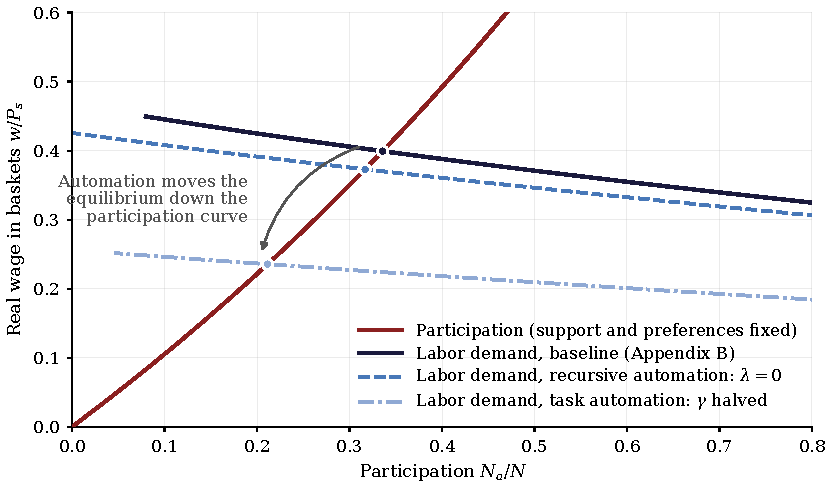
\includegraphics[width=0.88\textwidth]{figures/fig_labor_market_clearing.pdf}
\caption{Labor-market clearing in the numerical economy of Section~\ref{sec:example} ($N=1$, $T=0.01$, $h=0.0017$, $a=1.4$, $b=0.4$, $\delta=0.05$, $\rho=0.09$, $\chi$ uniform on $[0,2.2]$). The participation curve $N_a/N=\log(1+w/P_s)/2.2$ holds support and preferences fixed. Each demand curve traces labor demand $N_D/N$ against $w/P_s$ as the task margin moves over the tasks open to machines below the ceiling $x_c$. At baseline ($\lambda=7.3$, $\gamma(x)=0.01+0.99x^{4.4}$), the equilibrium has $w/P_s\simeq2.76$ and $N_a/N\simeq0.60$. Recursive automation ($\lambda=0$) moves it to about $2.46$ and $0.56$; task automation, which halves $\gamma$ at every task, moves it to about $2.66$ and $0.59$. Drawn by code written with Claude (Anthropic).}
\label{fig:3}
\end{figure}

% from main.tex L324, sentences 3-4 (the statics), edited: in sentence 4, "This participation response" ->
% "The participation response of Corollary~\ref{cor:statics}(ii)" (cross-reference: sentences 1-2, which it
% followed, are now Corollary 1 in Section 4); sentence 3 verbatim
Workers occupy tasks at which their relative productivity is higher. The participation response of Corollary~\ref{cor:statics}(ii) can cushion a wage decline from automation; the overall effect depends on how technology changes replacement costs and the living basket.
% NEW (design synthesis §3.4: the two experiments framed as artificial intelligence), in place of main.tex
% L324, sentence 5 ("Figure~\ref{fig:3} draws this market for the numerical economy of
% Appendix~\ref{app:B}."). Edited: the design's "this market" -> "the labor market" (its antecedent, the
% labor-market clearing of eq. (11), is now in Section 4)
Figure~\ref{fig:3} draws the labor market for the instance and for two experiments of Definition~\ref{def:automation}: recursive automation that removes labor from building machines ($\lambda=0$), as when chip design and datacenter operation are automated, and task automation that halves $\gamma$ at every task, as when models improve at every task at once.
% from main.tex L324, sentences 6-7, verbatim. Both channels lower w/P_s and N_a/N (2.757 -> 2.458 and
% 2.664; 0.6017 -> 0.5640 and 0.5903; work/07_08/recompute.py)
With support and preferences fixed, participation depends only on $w/P_s$, so technology moves only the demand side. In that example, both automation channels lower the real wage and participation together.
% NEW (design synthesis §3.4; code/appendix_b.py's header; STATE 2026-11-03), placed after the claim it
% qualifies. Recomputed in work/07_08/other_root.py: the two roots are 4.355 and 15.498, and at the upper
% one, calibrated to the same seven targets, halving gamma raises w/P_s by 9.2 percent (8.7 to 8.9 percent
% once rounded)
Of the two curvatures that match the targets, we take the lower; at the other, about $15.5$, task automation raises $w/P_s$.

% from main.tex L747, sentence 1, verbatim
For an illustrative automation path, retain these parameters and set $\lambda=0$ and $\gamma_\eta(x)=\eta(0.01+0.99x^{4.4})$, with $0<\eta\le1$; at $\eta=1$ this is the recursive-automation economy of Figure~\ref{fig:3}.
% from main.tex L747, sentence 2, edited: "The conditions in \eqref{eq:25} hold throughout" is verbatim, and
% its full stop gives way to the design's clause from ", since" on (NEW, design synthesis §3.4: why the
% conditions hold, and what Theorem 1 then gives)
The conditions in \eqref{eq:25} hold throughout, since with $\lambda=0$ and $H$ empty no labor is demanded at the ceiling $x_c=1$, while some is supplied at every positive wage; so by Theorem~\ref{thm:1} each economy on the path has at most one equilibrium, and has one when its support is funded.
% NEW (design synthesis §3.4), its second clause main.tex L747, sentence 3, verbatim from "equilibrium wage
% satisfies" on (the design joins it to its own clause, so "The" is lowercased; the bound is the anchor
% "path bound" of checks/check_interior.py). pi = 0.069652 (work/07_08/recompute_path.py)
% Review edit (R21): pi is identified with b~_m of (5)
With $\lambda=0$ the machine rental is $p_m=\pi r$ at every margin, where $\pi=(\rho+\delta)b/[1-(\rho+\delta)a]=\widetilde b_m$, and the equilibrium wage satisfies $0<v\le\eta(\rho+\delta)b/[1-(\rho+\delta)a]\to0$.
% NEW (design synthesis §3.4): funding proved for small eta and checked on a grid, in place of main.tex
% L747, sentence 6 ("The provider's rent and interest fund the support throughout."). (T-Nh)/(N pi) =
% 0.11916; rent and interest fund the support at all 2,001 points of a log grid on [1e-4, 1]
% (work/07_08/recompute_path.py)
Since $\gamma_\eta\le\eta$, $P_s\le(\eta\pi+h)r$, so rent alone funds the support whenever $\eta\le(T-Nh)/(N\pi)$, about $0.12$ here; rent and the return on machines fund it at every $\eta$ on a grid from $10^{-4}$ to $1$.
% from main.tex L747, sentences 4-5, verbatim (participation 0.5640 at eta = 1 and 0.1340 at eta = 0.01)
Relative capability remains a hundred times as high at the last task as at the first. Since $P_s\ge h>0$, participation tends to zero through \eqref{eq:24}: it is $0.56$ at $\eta=1$ and $0.13$ at $\eta=0.01$.
% NEW (design synthesis §3.4; STATE 2026-11-05): participation 0.017877 at eta = 0.001
At $\eta=0.001$ it is $0.018$.
% from main.tex L747, sentence 7, edited: "as in the proof of Lemma~\ref{lem:B.1}" -> "as in
% Proposition~\ref{prop:5}" (cross-reference: the income identity with interest is now Proposition 5).
% The design leaves this sentence out; it is kept because its content carries over (build brief §1, rule 1)
The purchasing-power bounds apply at every interior equilibrium along the sequence; income also includes interest, as in Proposition~\ref{prop:5}, and labor's share still tends to zero.
% NEW (design synthesis §3.4). R/I = 0.270 at eta = 1 and 0.9995 at 1e-4; from eta = 1 to 0.001, w/p rises
% by the factor 1.7804 and w/r falls by the factor 426.19 (work/07_08/recompute_path.py)
The machine stock satisfies $X\le\eta T/[h(1-a\delta)]$, so the return on machines vanishes relative to income and $R/I\to1$. From $\eta=1$ to $\eta=0.001$ an hour's wage comes to buy $1.8$ times as much of the final good and $1/426$ as much space: the real-wage fork of Proposition~\ref{prop:4} in its simplest form.

% ---- build part 08_measurement.tex (SP/build/parts/08_measurement.tex) ----
% =====================================================================================================
% Section 8. Measurement (sec:measurement). Build part 08, 2026-11-05.
% The authors' Section 9 (main.tex L475-528), verbatim (build brief §2, row 8). The only change in the source
% is the section label. Cross-references keep their labels (prop:4, fig:5, fig:6, fig:7, app:F), so the
% printed figure numbers change by themselves: old Figures 5-7 print as Figures 4-6, since Figure 3 is in
% Section 7 and old Figure 4 follows in Section 9. Notes: parts/07_08.notes.md.
% =====================================================================================================
% from main.tex L475, edited: \label{sec:9} -> \label{sec:measurement} (build brief §2: the section's new label)
\section{Measurement}\label{sec:measurement}

% from main.tex L477, verbatim
In this section we observe three empirical objects: the real-wage fork, the size of the rent base relative to the cost of a subsistence bundle, and the separation between the origin of consumption finance and the human effort embodied in production.

% from main.tex L479, verbatim (Proposition~\ref{prop:4} is the real-wage fork of Section 5; fig:5 keeps its label
% and prints as Figure 4)
\textbf{The fork.} Over 1964--2024, the durables-to-shelter real-wage ratio reaches $4.8\times$ (Figure~\ref{fig:5}). This descriptive comparison is consistent with the distinction in Proposition~\ref{prop:4} between task costs and persistent requirements for non-produced inputs. Identifying the underlying task schedules and attributing the price changes require additional task-level evidence. Food lies between the endpoints. Deflated by the food CPI, the same paycheck rose 13 percent over 1964--2024, compared with 277 percent for durables and a decline of 21 percent for shelter. The intermediate result is consistent with food production combining acreage, processing labor, and rising yields. Energy is volatile, consistent with the importance of world oil-price shocks in the series.

% from main.tex L481-492 (Figure 5, the deflator fork), verbatim: file, width, caption and label fig:5 unchanged;
% it prints as Figure 4
\begin{figure}[t!]
\centering
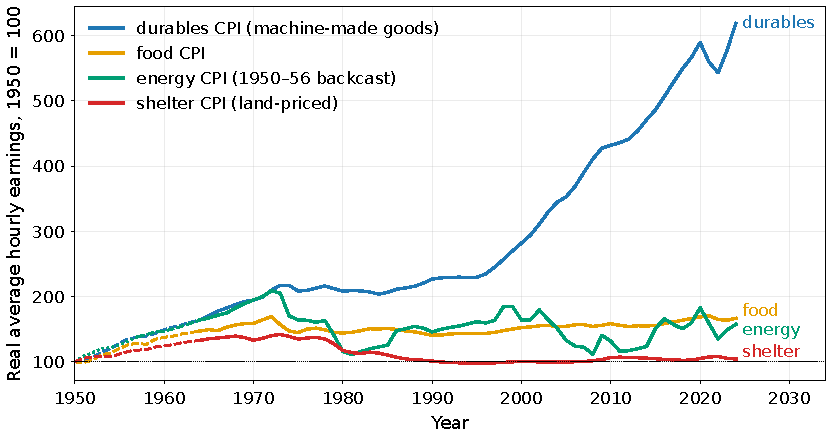
\includegraphics[width=0.88\textwidth]{figures/fig_deflator_fork.pdf}
\caption{U.S. average hourly earnings for production and nonsupervisory
workers deflated by the consumer-price indexes for durables, food, energy,
and shelter, 1950 = 100, through the last complete calendar year, 2024.
Values before 1964 (dashed) use the spliced wage series. The energy index begins in
1957; its 1950--1956 values are a linear backcast estimated over 1957--1966.
Over 1964--2024 the ratio of the durables-deflated to the shelter-deflated
wage reaches $4.8\times$, a ratio invariant to the index base. Drawn by code written with Claude (Anthropic).}
\label{fig:5}
\end{figure}

% from main.tex L494, verbatim (fig:6 prints as Figure 5)
\textbf{Coverage of basic living costs.} The coverage ratio $\kappa$ is the fraction of one subsistence bundle that a full tax on site rents could finance per person. Figure~\ref{fig:6} measures aggregate site-rent flow against population times a costed subsistence bundle. The 2025 estimate is $\kappa=0.30$ [0.15--0.59], up from roughly 0.05 in the 1950s. The measures are intended as lower-bound constructions. The underlying resource constraint is the non-produced input required by the basket relative to its available supply per person.

% from main.tex L496-511 (Figure 6, the coverage ratio), verbatim: label fig:6 unchanged; it prints as Figure 5
\begin{figure}[t!]
\centering
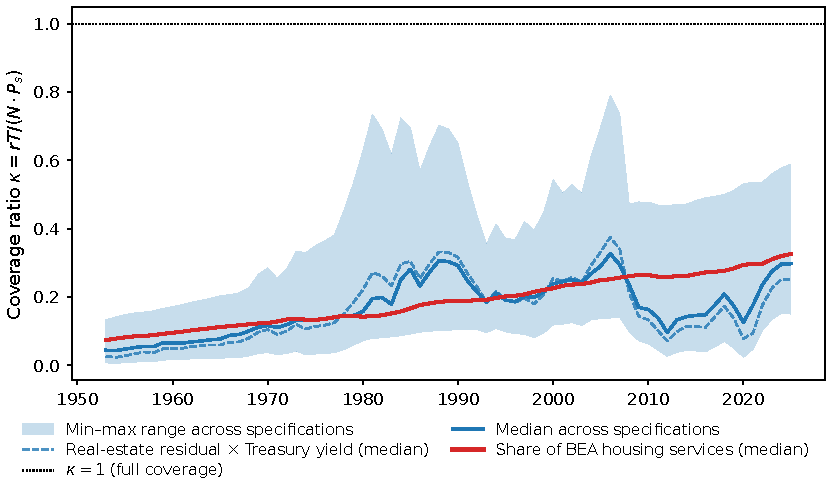
\includegraphics[width=0.88\textwidth]{figures/fig_kappa_measurement.pdf}
\caption{The coverage ratio $\kappa=rT/(N\cdot P_s)$ is aggregate site-rent flow divided by the cost of providing the specified subsistence bundle to every person; U.S., 1953--2025. The
line is the median and the band is the min--max range across specifications
combining land sources, capitalization rates, and subsistence bundles. The
dashed specifications subtract residential structures at replacement cost
(Z.1, BOGZ1LM155012665Q) from household real estate at market value (Z.1,
FRED HOOREVLMHMV) and convert the residual to an annual flow using the 10-year
Treasury yield (GS10), with a +150 basis-point variant and household and
economy-wide scopes. The red specifications apply land shares of 0.30 and
0.50 to PCE housing services (BEA, DHSGRC1A027NBEA). Every specification
uses population times the Orshansky 1963 subsistence bundle as the
denominator. Drawn by code written with Claude (Anthropic).}
\label{fig:6}
\end{figure}

% from main.tex L513, verbatim (fig:7 prints as Figure 6; app:F is Appendix F, the financing and production
% accounts, as before)
\textbf{Financing versus production.} Consumption remains substantially more labor-financed than production is labor-intensive. In the common benchmark-data window, labor-origin resources finance 69.6\% of consumption in 2004 and 65.8\% in 2023, while full-chain human effort accounts for 48.9\% and 47.2\% of consumed production in the same years --- a gap of about nineteen percentage points at the end of the overlap (Figure~\ref{fig:7}). The production account is the aggregate counterpart of the recursion: the human-effort share declines as machine-producing and machine-operating chains shed labor. Appendix~\ref{app:F} gives the two accounts' construction and bounds.

% from main.tex L515-528 (Figure 7, financing and human effort), verbatim: label fig:7 unchanged; it prints as
% Figure 6
\begin{figure}[t!]
\centering
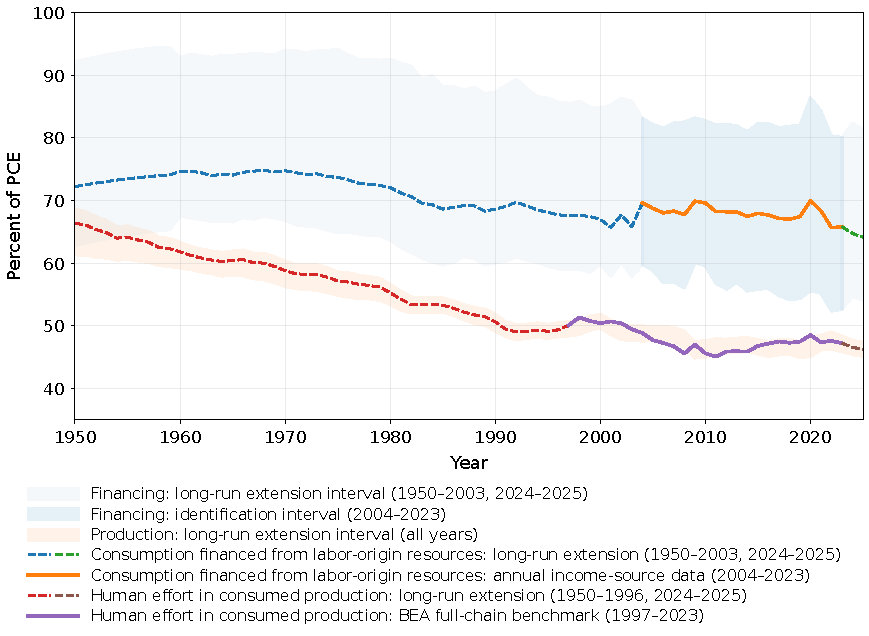
\includegraphics[width=0.92\textwidth]{figures/fig_consumption_financing_and_human_effort.pdf}
\caption{Two labor linkages in U.S. consumption, 1950--2025. The upper
series is the share of consumption financed from labor-origin resources; the
lower is the share of consumed production that resolves into human effort
through the full production chain. Solid lines identify the benchmark-data
windows: annual BEA income-source profiles for financing in 2004--2023 and
the BEA full-chain production benchmark in 1997--2023. Values outside those
windows are model-based extensions. In the common benchmark-data window,
consumption is substantially more labor-financed than production is
labor-intensive. Drawn by code written with Claude (Anthropic).}
\label{fig:7}
\end{figure}

% ---- build part 09_history.tex (SP/build/parts/09_history.tex) ----
% =====================================================================================================
% Section 9. History and stabilizers (sec:history). Build part 09, 2026-11-05.
% 9.1 opens with main.tex L326 (heterogeneity and skill premia), moved verbatim from the old Section 5 (design
% synthesis §1.1 and §1.3). Then the authors' Section 8 (L441-473), shortened by cuts of whole sentences only:
% its prose goes from 613 to 401 words (65 percent; caption and headings not counted), and it keeps its figure
% (old Figure 4, label fig:4, printed as Figure 7) and its four configurations (pre-industrial, industrial,
% post-industrial, and the candidate AI configuration inside the post-industrial paragraph, as before). One
% sentence is edited: L473's two-type wage ratio is stated as a conditional (design synthesis §3.7; inventory
% R21). 9.2 is the authors' Section 10 (L530-536) with one edit (L532: "most workers", Appendix E's own words, for
% "the median worker"; inventory R21) and one NEW sentence that names a reservation as a policy (design synthesis
% §4, decision 3). Every cut and edit is listed in parts/09_10.notes.md.
% =====================================================================================================
% NEW (build brief §2, row 9: the section's title and label)
\section{History and stabilizers}\label{sec:history}

% from main.tex L441, edited: section -> subsection (it is now 9.1); label sec:8 -> sec:configurations (new
% section labels, build brief §2)
\subsection{History as four configurations of the model}\label{sec:configurations}

% from main.tex L326, verbatim, moved from the old Section 5 (design synthesis §1.3: "Heterogeneity (326) | §8.1
% opening"; build brief §2, row 9)
% Review edit (D91): "active (contestable) margin" -> "interior margin", the name Definition 2 gives it
\textbf{Heterogeneity and skill premia.} Workers differ in task productivity, access to support, living costs, and preferences. An interior margin prices each type's wage against machine services. For a type employed only at human-required tasks in $H$, demand, supply, institutions, and participation determine the wage. Relative wages also reflect substitution between worker types and their relative supplies. Training takes time and resources; open entry disciplines the long-run premium through those costs, while shortages can sustain a higher return. These comparisons guide the historical discussion. A full account of skill premia would jointly determine assignment, training, and household labor supply.

% from main.tex L443, sentences 1-3, verbatim; sentence 4 cut (L326's last sentence, now just above, says it, and
% its pointer, to the old Section 5 (label sec:5), was to L326; notes (c))
The model can be applied to the long record as four configurations of the relative-productivity schedule (Figure~\ref{fig:4}). Because schedules may differ across worker types, the figure shows each configuration for both an untrained entrant and a worker with accumulated training or experience. Both face the same wall, since which tasks are in $H$ does not depend on the worker; training changes a worker's schedule and wage.

% from main.tex L445-467, verbatim: old Figure 4, its label fig:4 kept (build brief §2, labels); it prints as Figure 7
\begin{figure}[t!]
\centering
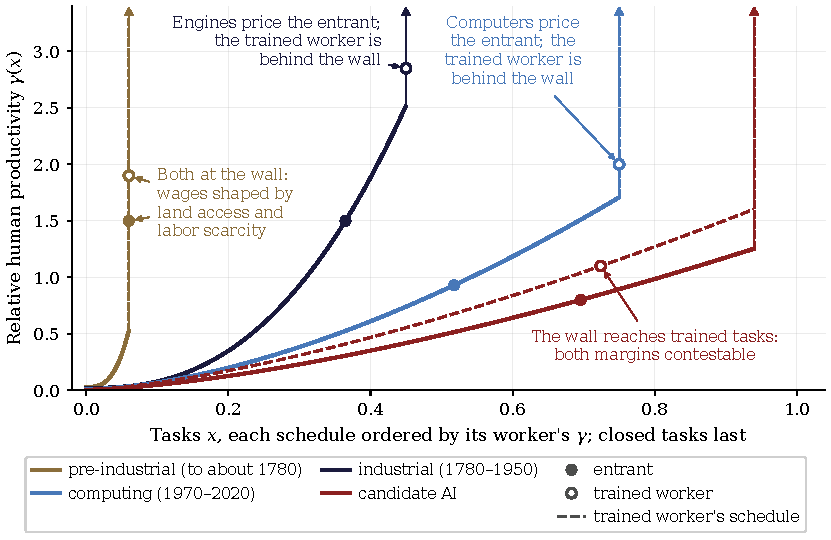
\includegraphics[width=0.88\textwidth]{figures/fig_eras_workers.pdf}
\caption{Four schematic configurations of the task schedule, shown for
an untrained entrant (filled dots) and a worker with accumulated training or
experience (open dots). Solid curves are the entrant's schedules; the trained
worker's own schedule is drawn (dashed) only in the candidate AI configuration, and
in the others lies below that worker's wage ratio at every open task. Closed tasks
appear as a wall at the right edge, common to both workers. Dot heights are
illustrative wage--machine-rental ratios $w/p_m$; within a configuration both dots
share $p_m$, so their ratio is the illustrative training premium. A dot on a
schedule marks an interior margin satisfying $w/p_m=\gamma(x^*)$; a dot on the wall
marks employment confined to human-required tasks, whose wage also depends on
demand, labor supply, and institutions. Industrialization opens physical tasks;
computing extends competition into cognitive tasks while many trained tasks remain
closed. Relative human advantage continues to vary across the open task range. In
the candidate AI configuration, machine competition extends across more tasks,
including trained ones, and the trained worker acquires an interior margin; the
schedules keep rising and retain an illustrative positive training premium. The
chosen curvatures illustrate differences in relative capability across tasks.
Drawn by code written with Claude (Anthropic).}
\label{fig:4}
\end{figure}

% from main.tex L469, verbatim (build brief §5: Ricardo and Malthus stay named without years; leave 469 verbatim)
\textbf{Pre-industrial: land access and labor scarcity.} With machines scarcely present, nearly every task is closed to them; the margin sits at the wall for entrant and master alike, so the machine prices no one's hour. Demand for human services, labor scarcity, institutions, and participation then determine wages. A configuration with wages near the outside option additionally invokes demographic adjustment, with the outside option tracking access to land --- the world Ricardo and Malthus wrote down, and the one long-run estimates describe: pre-industrial English real wages strongly shaped by population and land, with productivity growth beginning well before wages escaped Malthusian pressure (Bouscasse, Nakamura, and Steinsson 2025). The classical account is one configuration of our model. The entrant is the farm servant hired by the year; the trained worker is the craftsman after a seven-year apprenticeship, whose premium over the servant is the cost of those years, recovered.

% from main.tex L471, sentences 1, 2, 5 and 6, verbatim; sentences 3, 4 and 7 cut (notes (c)). Sentence 5 cites
% Proposition 1(ii), which part 04 keeps as prop:1 (ii)
\textbf{Industrial: comparative advantage widens.} The Industrial Revolution created a large and uneven productivity gap across tasks: engines were far better than muscle at physical tasks but ineffective at cognitive ones. The schedule became enormously dispersed and steep. That dispersion opened high-productivity tasks to labor and could support a higher wage; by Proposition~\ref{prop:1}(ii), steepness also makes employment less responsive to a given wage change and the wage more responsive to shifts in labor supply. Meanwhile machine production itself remained labor-intensive: both relative human productivity at the margin and the labor embodied in machine services supported the wage.

% from main.tex L473, sentences 1, 4 and 6, verbatim; sentences 2, 3 and 5 cut (notes (c))
\textbf{Post-industrial: machine competition broadens.} Computerization reached the simple-cognitive region of the schedule --- the routine-task evidence of Autor, Levy, and Murnane (2003) and the polarization it produced (Autor and Dorn 2013) are the cross-sectional trace. AI is a candidate extension of machine competition to further tasks, including those previously closed to machines. As trained tasks become contestable, skill premia depend on the replacement costs and labor supplies of the different worker types.
% from main.tex L473, sentence 7, edited: "Where the trained worker and the entrant both hold contestable margins
% against the same machine, Proposition 1(i) applies to each and the rental cancels" -> "If the trained worker and
% the entrant both held contestable margins against the same machine, Proposition 1(i) would apply to each and the
% rental would cancel" (the ratio stated as a conditional, the minimum change: the stated
% economy has one worker type and gives no two-type assignment; design synthesis §3.7; inventory R21; build brief
% §2, row 9). Sentence 8 cut (notes (c))
% Review edit (L1404): "contestable margins" -> "interior margins", as D91
If the trained worker and the entrant both held interior margins against the same machine, Proposition~\ref{prop:1}(i) would apply to each and the rental would cancel: $w_{\mathrm{tr}}/w_{\mathrm{en}}=\gamma_{\mathrm{tr}}(x^*_{\mathrm{tr}})/\gamma_{\mathrm{en}}(x^*_{\mathrm{en}})$.

% from main.tex L530, edited: section -> subsection (it is now 9.2); label sec:10 -> sec:stabilizers (new
% section labels, build brief §2)
\subsection{Possible stabilizers}\label{sec:stabilizers}

% from main.tex L532, sentences 1-3; sentences 1 and 3 verbatim; sentence 2 edited: "while leaving the median
% worker exposed" -> "while leaving most workers exposed" (inventory R21: Proposition E.1 says nothing about the
% median worker; Appendix E's own words, main.tex L890, are "most workers receive no income from its protected
% tasks"; the design's wording, "; most workers can still be exposed", is the alternative, notes (d))
Several mechanisms can sustain purchasing power as technology changes. Human-required tasks can persist by preference or by law; Appendix~\ref{app:E} shows that this can preserve aggregate labor income while leaving most workers exposed. Institutions can reserve tasks for people outright, protecting employment through an allocation rule.
% NEW (design synthesis §4, decision 3: H is closed by capability or by rule, and lifting a reservation is a policy
% change that the stabilizers subsection must name; build brief §2, row 9). Section 3.5 (sec:government) records a
% law that reserves tasks as a policy, and Definition 3 (def:automation) keeps the reserved tasks unchanged
Such a reservation is a policy (Section~\ref{sec:government}), and Definition~\ref{def:automation} does not count lifting it as automation.
% from main.tex L532, sentences 4-5, verbatim
Supply expansion --- building, densifying, powering --- works through the cost system by expanding services or reducing the scarce inputs required to supply them. Lower living costs can improve affordability, while cheaper machine services also affect replacement values.

% from main.tex L534, verbatim
Substitution can also change the services people choose. Replacing a journey and an in-person meeting with a video call changes the bundle of transport, space, equipment, and electricity used to communicate. Its resource requirements depend on those services' full production chains and on how well they meet the same need. The participation comparison holds the living basket fixed; consumer substitution can change its composition across equilibria.

% from main.tex L536, verbatim (the wedge; Section 3's wedge remark points here)
Acemoglu and Restrepo's (2026) wedge result clarifies the role of wage premia. Let a task pay a premium over the base wage --- a union premium, a licensing rent, an efficiency wage --- as a multiplicative wedge $\mu (x) > 1$. Labor then holds the task only while $w \le p_m\cdot \gamma (x)/\mu (x)$: allocation runs on the wedge-deflated schedule, a premium raises its own task's flip priority one-for-one, and automation is directed at the best-paid versions of each job --- their targeting result, with the documented losses concentrated in the 70th--95th within-group percentiles. A wage premium therefore increases the incentive to automate the protected task; protection survives only in quantity form --- a scope-of-practice rule extended to software, an enforceable automation ban, a mandated human in the loop. Under pressure, nothing moves while the saving from flipping runs below the cost of confrontation with a legal or strike risk; past it, everything the rule covers flips at once.

% ---- build part 10_ai.tex (SP/build/parts/10_ai.tex) ----
% =====================================================================================================
% Section 10. Artificial intelligence and conclusion (sec:ai). Build part 10, 2026-11-05.
% The authors' Section 11 (main.tex L538-550), less what the design moved to Section 3: L540's sentences 1-2 stand
% verbatim in Section 3's AI paragraph, and its sentences 6-7 are restated there (part 03; design synthesis §3.7:
% "Its mapping moves to §2.6 and §1; §9 keeps the purchasing-power reading"). The rest is verbatim but for two
% cross-references in L540. The Leontief aside (build brief §6) stands directly after L542's rent-tax sentence.
% Then the authors' Section 12, Future Work (L552-559), condensed by cuts to two paragraphs and folded into this
% section (STATE Open 12(k): "Future Work" after the conclusion; design synthesis §1.3): the monetary-policy passage
% (L553, sentences 4-8) and the sovereign-fund passage (L557, sentences 5-7) keep one sentence each (design synthesis
% §1.5). The design's Uzawa (1961) sentence is not added (build brief §5 drops Uzawa). Notes: parts/09_10.notes.md.
% =====================================================================================================
% from main.tex L538, edited: label sec:11 -> sec:ai (build brief §2)
\section{Artificial intelligence and conclusion}\label{sec:ai}

% from main.tex L540, sentences 3-5 (sentences 1-2 stand verbatim in Section 3's AI paragraph and sentences 6-7 are
% restated there, so they are left out here; build brief §2, row 10). Edited: (a) sentence 3, a cross-reference to
% Definition 3 (label def:automation) added after "Either change", whose antecedent, sentences 1-2, is now in
% Section 3 (part 04 adds the same pointer to L251's "either channel"); (b) sentence 4, the section pointer sec:6 ->
% sec:purchasing (old Section 6, "Purchasing power at an interior margin", is now Section 5)
% Review edit (D91): "active (contestable) margin" -> "interior margin", the name Definition 2 gives it
Either change (Definition~\ref{def:automation}) lowers $w/r$ when the other terms in the replacement closure are held fixed; the equilibrium effect also depends on demand, participation, and changes in the recipes. Section~\ref{sec:purchasing} translates that ratio into purchasing power through the labor and non-produced inputs embodied in goods and services. If replacement at the interior margin drives $w/r$ toward zero while an embodied non-produced input requirement remains bounded away from zero, wage command over that output falls toward zero.

% from main.tex L542, sentences 1-6, verbatim
% Review edit (D74): L542 sentence 2: pointer to Corollary 2 added
On the household side, falling wage purchasing power reduces the consumption gained from employment relative to a supported living standard. Participation helps determine which task is marginal and, with support maintained and positive work costs, tends to zero as wages buy vanishing additional consumption (Corollary~\ref{cor:vanishing}). Maintaining that standard depends on the resources of families and public institutions. Rent income provides a potential fiscal base. For the measured U.S. site-rent base, full capture covers about 30 percent of the specified subsistence bundle in 2025, while 0.68 of tax revenue is raised from labor-income bases. A tax on pure fixed-factor rents can fund a payment paid equally in and out of work; the coverage ratio determines whether it can finance the full basket.
% NEW (build brief §6: the aside, exact text decided by Stella; STATE 2026-11-05, C14 with "the model makes precise"
% taken out), directly after "A tax on pure fixed-factor rents can fund a payment paid equally in and out of work;
% the coverage ratio determines whether it can finance the full basket." as the brief says
Leontief (1983) compared the future of human labor to that of horses after the tractor. The comparison fails in one respect: people, unlike horses, can vote for a rent dividend.
% from main.tex L542, sentence 7, verbatim
Its scale, income effects, and equilibrium consequences remain empirical questions.

% from main.tex L544-546, verbatim
The remaining empirical question is whether the machine-production recursion
is paying a smaller share of cost to wages and a larger share to
terminal-input rents, and whose resources are keeping pace with the resulting cost of living outside paid work.

% from main.tex L548, verbatim
We close with a conjecture that the model suggests but does not establish. Wages finance most consumption, and most benefits are conditioned on work or means. When consumption depends on earning a wage, a lower wage need not reduce the labor offered, so the economy has little way to signal that it wants less labor, as it can for oil in a glut or for capital when returns approach zero. Labor may then have been behaving for decades as a large market distortion: jobs are created at cost, behind institutional wedges or at wages barely above living costs. If the conjecture holds, it would connect developments usually studied separately, including polarized job growth, youth unemployment, delayed household formation, persistent fiscal strain, and slow growth despite rapid advances in computing. Each needs its own test. The first is whether machine production is shifting its costs from wages to rents.

% from main.tex L550, verbatim
The mechanism also joins older lines of thought. The classical economists tied wages to subsistence and scarcity, George drew the fiscal consequences of rent, and Keynes (1936) put employment and demand at the center of the economy. Automation that reaches the machines' own supply chains gives them a common setting, and perhaps a common wage equation.

% from main.tex L553, sentences 1-3 and 7, verbatim. The heading "Future Work" (L552, label sec:12) is dropped: Future Work is folded into this section (STATE Open 12(k)). Sentences 4-6 and 8 cut: the monetary-policy
% passage (sentences 4-8) keeps one sentence, its question on low interest rates (build brief §2, row 10; design
% synthesis §1.5; notes (c), (d))
% Review edit (D73): L553: "static" -> "stationary" (Section 3 defines a stationary equilibrium with an infinitely lived owner)
There is much still to be done. The stationary model describes prices and limiting configurations. A dynamic extension could ask whether automation arrives smoothly or in waves, how quickly rents adjust, and what happens when wages fall faster than institutions can respond. Do low interest rates support employment and demand, or do they mainly raise scarce-asset rents and accelerate the replacement of labor?
% from main.tex L555, verbatim (joined to L553 to make the first of the two Future Work paragraphs)
Participation also invites further study. The benchmark holds real support fixed. A richer account would let families and public institutions adjust provision as living costs and their own resources change. Personal assets, pensions, and savings would add further ways to sustain life outside employment. Richer household structure would open further questions. If wages buy ever more manufactured goods but ever less housing, energy, and care, then forming a household may become harder even while measured productivity rises. Delayed household formation, adult children remaining with their parents, and declining fertility may therefore reflect changing preferences alongside a growing separation between wages and the scarce goods required to begin an independent life.

% from main.tex L557, sentences 1-4 and 7, verbatim; sentences 5-6 cut: the sovereign-fund passage (sentences 5-7)
% keeps one sentence, its last (build brief §2, row 10; design synthesis §1.5; notes (c), (d))
The model also suggests avenues for choosing the tax mix as automation changes the sources of income. Labor and ownership both finance consumption, and site rents may cover only part of a desired transfer. The relevant question is the best mixture of value-added, income, corporate, land-value, and other pure-rent taxes. Our input-output and consumption financing measurements may help significantly with this. For resource-poor countries, owning part of the world’s scarce-resource base may eventually matter as much as taxing the domestic one.
% from main.tex L559, verbatim (joined to L557 to make the second Future Work paragraph)
Finally, structuring a society that no longer orbits around labor is not a trivial problem. Work provides more than a wage. It provides structure to the day, social contact, status, a sense of contribution, and an understanding of the complexity of the real economy. An income transfer can replace a wage; it cannot by itself replace all of those functions. Some may emerge naturally through family, community, education, art, care, or voluntary work. Others may have to be deliberately nurtured. The economic problem may be how to distribute purchasing power without labor. The larger human problem is how to distribute purpose, status, and a meaningful place in society once labor is no longer the institution that provides them.

% ---- build part 11_appA.tex (SP/build/parts/11_appA.tex) ----
% =====================================================================================================
% Appendix A. Proofs (app:proofs). Build part 11, 2026-11-05.
% Opens the appendices with main.tex's appendix switch (L561-566), with the lemma, assumption and
% definition counters added beside L562-565 (build brief §3; design synthesis §2.0).
% Built from design synthesis §3.5: Lemma A.1 with fix F4 in part (a) and fix F5 in the remark on part (c),
% and the drafted proofs. The authors' proofs stand wherever their content carries over: main.tex L729-740
% (Lemma B.1's proof, now in Theorem 1's), L743 (Corollary 1(ii)), L647 and L370-371 (Proposition 4 and
% Corollary 2), L389-391 with L751-757 (Proposition 5, with Appendix C's identity and the interest term),
% L413-415 (Proposition 6) and L769-775 (Corollary 3). The general human-method bound (19) and the
% network versions of these proofs are in Proposition B.1 (part 12). Notes: parts/11_12.notes.md.
% =====================================================================================================

% from main.tex L561-566 (the appendix switch), edited: \counterwithin{lemma}, {assumption} and
% {definition} added beside L562-565 (build brief §3; design synthesis §2.0), so that they print as
% Lemma A.1, Assumption B.1 and Definition B.1
\appendix
\counterwithin{proposition}{section}
\counterwithin{lemma}{section}
\counterwithin{assumption}{section}
\counterwithin{definition}{section}
\counterwithin{equation}{section}
\counterwithin{figure}{section}
\counterwithin{table}{section}
\titleformat{\section}{\normalfont\Large\bfseries}{Appendix~\thesection.}{0.6em}{}

% NEW (design synthesis §3.5): the title and label of Appendix A. They replace main.tex L568 ("The
% environment and supporting results", app:A); that environment is now Section 3, and its extensions are
% Appendix B
\section{Proofs}\label{app:proofs}

% NEW (design synthesis §3.5), with fix F4 (build brief §4). Part (a) was "If $r>0$, every optimal plan
% rents out $\ell_t=T$ in every period", which is false at beta = 1 under the long-run-average criterion;
% (a) is now F4's wording. The clause defining a feasible plan is added (NEW): the proof uses its
% constraints, and Definition 1(iii) leaves them implicit
\begin{lemma}[the owner's problem]\label{lem:owner}
Take constant prices with $P_s>0$ and $V_m>0$, a machine-hour rental $p_m$, and a policy with $\tau_R\in[0,1]$, and call a plan feasible if it satisfies~\eqref{eq:ownerseq} with $0\le\ell_t\le T$, $X_t\ge0$, and $c_{o,t}\ge0$ in every period.
(a) If $\beta<1$, every optimal plan rents out $\ell_t=T$ in every period when $r>0$; when $\beta=1$, every optimal constant plan does.
(b) If $p_m=(\rho+\delta)V_m$, the constant plan that rents out $\ell$ (with $\ell=T$ if $r>0$), holds the stock $X$, and consumes $c_o=[r\ell-\tau_RrT+\rho V_mX]/P_s-\sigma N$ in every period is optimal from the initial stock $X$ whenever $c_o\ge0$.
(c) If a constant plan with $X>0$ and $c_o>0$ is optimal at a rental $p_m$, then $p_m=(\rho+\delta)V_m$: the user cost is the owner's first-order condition.
\end{lemma}

% NEW (design synthesis §3.5). Edited: (a) for fix F4, with the beta = 1 case argued on constant plans;
% (b) the budget is written as an inequality for every feasible plan, since a plan may rent out less land
% than the constant one, and the beta = 1 bound is stated for the limit superior of average utility, since
% the average need not converge (math check C5)
\begin{proof}
(a) The land tax $\tau_RrT$ does not depend on $\ell_t$, so renting out more land raises the period's resources whenever $r>0$, and $u$ is strictly increasing. If $\beta<1$, a plan that rents out less than $T$ in some period is therefore improved by renting out $T$ in that period and consuming the extra rent then. If $\beta=1$, a constant plan with $\ell<T$ is improved by the constant plan that rents out $T$ and consumes $r(T-\ell)/P_s$ more in every period. Changes in finitely many periods leave the long-run average unchanged, so for $\beta=1$ the claim concerns constant plans.
(b) Write $W_t=V_mX_t\ge0$ and $y_o=r\ell-\tau_RrT-\sigma NP_s$. At the user cost, \eqref{eq:ownerseq} gives $W_{t+1}\le(1+\rho)W_t+y_o-P_sc_{o,t}$ for every feasible plan, since $r\ell_t\le r\ell$, with equality for the constant plan; let $c^*=(\rho W_0+y_o)/P_s\ge0$ be the constant plan's consumption. For $\beta<1$, summing the budget with weights $\beta^t$ and using $W_t\ge0$ gives $\sum_t\beta^tc_{o,t}\le\sum_t\beta^tc^*$ for every feasible plan; since $u$ is concave and increasing, Jensen's inequality with the weights $(1-\beta)\beta^t$ gives $\sum_t\beta^tu(c_{o,t})\le\sum_t\beta^tu(c^*)$. For $\beta=1$, the budget gives $\frac{1}{t_1}\sum_{t<t_1}c_{o,t}\le c^*+W_0/(t_1P_s)$ for every horizon $t_1$, and concavity and continuity bound the limit superior of average utility by $u(c^*)$. In both cases the constant plan attains the bound.
(c) If $p_m>(\rho+\delta)V_m$, cutting consumption by $\varepsilon$ in one period and spending it on machines raises the next period's consumption by $(1+p_m/V_m-\delta)\varepsilon>(1+\rho)\varepsilon$, a first-order gain since $u'>0$; if $p_m<(\rho+\delta)V_m$, the reverse change gains. Both are feasible because $c_o>0$ and $X>0$. With $\beta=1$, the first change raises consumption in every later period, and the second, which buys fewer replacement machines once, raises it in every later period, so each raises the long-run average.
\end{proof}

% NEW (build brief §7: after each result, a remark on what it does not depend on), for fix F5 (build brief
% §4): Lemma A.1(c) gives the user cost only when the owner consumes and holds machines, and Definition 1(i)
% keeps the user-cost clause. The middle sentence gives the reason the first-order condition does not bind
% at c_o = 0 (math check C5: the shortfall D_{t+1} >= (1+g)D_t at net return g > 0); the last is F5's plain
% sentence, which Sections 3 and 4 also print. Nothing here says that the clause "costs nothing"
% Review edit (mathA-2): at zero rent the owner can vary the land it rents out, so the constant plan is not its only feasible plan; what the shortfall argument proves is that no feasible plan has other consumption or stock
\begin{remark}
Lemma~\ref{lem:owner} takes prices as given, so it does not depend on technology or on market clearing. Part~(c) needs $c_o>0$ and $X>0$. When support absorbs all the owner's income at a rental above $\delta V_m$, so that $c_o=0$, the owner has no feasible plan with other consumption or stock, since any such departure leaves a shortfall in wealth that grows at the net return $p_m/V_m-\delta$. The first-order condition then does not bind, and the user-cost clause of Definition~\ref{def:equilibrium}(i) selects the user cost at~$\rho$.
\end{remark}

% NEW (design synthesis §3.5). Edited: in (iii), the design's pointer "as in main.tex 737--738" is replaced
% by the computation it points to (main.tex L738's display, read at any margin), and the comparison of the
% coefficients is spelled out
\begin{proof}[Proof of Lemma~\ref{lem:prices}]
(i) The matrix $\mathbf A_\rho$ in~\eqref{eq:3} has spectral radius $\sqrt{(\rho+\delta)a}<1$ by Assumption~\ref{ass:machines}, so $(\mathbf I-\mathbf A_\rho)^{-1}=\sum_{t\ge0}\mathbf A_\rho^t\ge\mathbf 0$; its machine-hour row gives~\eqref{eq:tildem}, and $\mathbf z^{\top}$ applied to~\eqref{eq:4} gives $P_s$. (ii) Definition~\ref{def:equilibrium}(v): $X=YJ(x^*)/(1-a\delta)$, so labor and land are $YL_s$ and $YB_s$. (iii) Since $(\rho+\delta)/[1-(\rho+\delta)a]\ge\delta/(1-\delta a)$, with equality when $\rho=0$, comparing~(i) with~(ii) term by term gives the inequalities. By~\eqref{eq:unitcost} and Definition~\ref{def:equilibrium}(v), $pY=w(N_a-\lambda\delta X)+p_m(1-a\delta)X$ and $hrY=r(\ell-b\delta X)$, so $P_sY=wN_a+r\ell+(p_m-\delta V_m)X=wN_a+r\ell+\rho V_mX$; dividing by $Y=C\ge N>0$ and using~(ii) gives the identity.
\end{proof}

% NEW (design synthesis §3.5). Edited: one sentence added that D does not increase, so that D <= 0 on all
% of [x_c, x_H], and one that machines perform no task in H, which the claim about [x_c, 1] needs
\begin{proof}[Proof of Lemma~\ref{lem:ceiling}]
By~\eqref{eq:unitcost}, $p_m\gamma(x)-w=[(\rho+\delta)br\gamma(x)-wD(x)]/[1-(\rho+\delta)a]$, with $D(x)=1-(\rho+\delta)(a+\lambda\gamma(x))$. Since $\gamma$ increases, $D$ is nonincreasing, so $D\le0$ on $[x_c,x_H]$ when some open task has $D(x)\le0$. Where $D(x)\le0$ the difference is nonnegative, and it is zero only if $r=0$ and $D(x)=0$, at a single task because $\gamma$ increases strictly, or if $w=r=0$, which would make every price zero. So machines perform almost no task in $[x_c,x_H]$, and Definition~\ref{def:equilibrium} gives them none in $H$. Assumption~\ref{ass:machines} gives $D(0)>0$, so $x_c>0$.
\end{proof}

\begin{proof}[Proof of Theorem~\ref{thm:1}]
% from main.tex L729-734 (the first paragraph of Lemma B.1's proof), edited: n_D and n_S renamed N_D and
% N_S (Table 1)
The function $Y(x)$ is decreasing. Below $x_c$, $\delta(a+\lambda\gamma(x))\le(\rho+\delta)(a+\lambda\gamma(x))<1$, so the bracket in labor demand is positive and has derivative $-1+\lambda\delta\gamma(x)/(1-a\delta)<0$; $N_D(x)$ is strictly decreasing. Meanwhile $v'(x)>0$ and
\begin{gather*}
p'(x)=v'(x)\left[1-x+\frac{(\rho+\delta)\lambda J(x)}{1-(\rho+\delta)a}\right]>0,\\
\frac{d}{dx}\left(\frac{v(x)}{P_s(x)}\right)=\frac{v'(x)\,[h+(\rho+\delta)bJ(x)/(1-(\rho+\delta)a)]}{P_s(x)^2}>0
\end{gather*}
for $0<x<x_c$. Thus $N_S(x)$ is continuous and nondecreasing up to its limit at $x_c$. Since $J(0)=0$, demand at $x=0$ is $T/h>N$, above supply; at $x_c$ it lies below supply by assumption. There is exactly one crossing.

% NEW (design synthesis §3.5, "Proof that every equilibrium of Theorem 1 is interior, with w > 0 and r > 0").
% Edited for fix F5: the zero-rent step names the user cost of Definition 1(i), on which it rests (the
% sentence after Theorem 1 in Section 4 says the proof uses it). Edited for fix F4: land is fully used
% because the owner's plan is constant, the case Lemma A.1(a) covers at every beta
Take an equilibrium. By Definition~\ref{def:equilibrium}(i) and Lemma~\ref{lem:ceiling}, up to measure zero machines perform an initial segment $[0,x^*)$ of the open tasks, with $x^*\le x_c$.
\emph{The wage is positive.} If $w=0$, almost no worker works, since $F(0)=0$. If also $r=0$, every price is zero by~\eqref{eq:4}, contradicting $P_s>0$. If $r>0$, then $p_m>0$ because $b>0$, labor is strictly cheaper at every task, and labor demand is at least $Y=C\ge N>0$.
\emph{The rent is positive.} Suppose $r=0$. By~\eqref{eq:tildem}, which rests on the user cost of Definition~\ref{def:equilibrium}(i), $p_m=w\widetilde\lambda_m$, so machines are cheaper exactly at the open tasks where $\gamma(x)\widetilde\lambda_m<1$, and $x^*=x_c$. If $\lambda=0$ and $H$ is empty, every price but $w$ is zero and $P_s=0$. Otherwise $w/P_s=1/[1-x_c+\widetilde\lambda_mJ(x_c)]$. This is at least the limit of $v/P_s$ as the margin rises to $x_c$: equal to it when $\gamma(x_c)\widetilde\lambda_m=1$, and larger when $\gamma(x_c)\widetilde\lambda_m<1$, which requires $x_c=x_H$. So at least $N_S(x_c)$ hours are supplied. Land used, $YB_s(x_c)$, cannot exceed $T$, so at most $TL_s(x_c)/B_s(x_c)=N_D(x_c)$ hours are employed, and $N_D(x_c)<N_S(x_c)$ by~\eqref{eq:25}.
\emph{The margin is interior.} With $r>0$, Lemma~\ref{lem:owner}(a) gives $\ell=T$ for the owner's constant plan, so land is fully used. If $x^*=0$, no machine is used, $Y=T/h$, and labor demand $T/h$ exceeds $N$. If $x^*=x_c$ and $\gamma(x_c)\widetilde\lambda_m=1$, cost minimization needs $w\ge v(x)r$ for almost every $x<x_c$, and $v(x)\to\infty$ as $x$ rises to $x_c$. If $x^*=x_c=x_H$ and $\gamma(x_H)\widetilde\lambda_m<1$, the assignment is a boundary assignment with $w\ge v(x_H)r$. There $P_s=w[1-x_H+\widetilde\lambda_mJ(x_H)]+r[h+\widetilde b_mJ(x_H)]$, so $w/P_s$ rises with $w$ and is at least its value at $w=v(x_H)r$. Hence at least $N_S(x_c)$ hours are supplied, against a demand of $N_D(x_c)$, and~\eqref{eq:25} gives excess supply.

% NEW (design synthesis §3.5). Edited: the design's "the remaining conditions hold as in the verification
% of main.tex 736--740" now introduces that verification, which follows
So $0<x^*<x_c$. By Propositions~\ref{prop:1} and~\ref{prop:2}, prices are \eqref{eq:21}--\eqref{eq:22} at $x^*$; quantities follow from Definition~\ref{def:equilibrium}(v) as in \eqref{eq:23}--\eqref{eq:24}; and labor-market clearing selects the unique crossing. If the owner's income covers the support at $x^*$, Lemma~\ref{lem:owner}(b) makes its constant plan optimal, and the remaining conditions hold, as follows.

% from main.tex L736-740 (the second paragraph of Lemma B.1's proof), edited: "provider" renamed "owner"
% twice (the agent of Assumption 5; design synthesis §3.7 renames it at L745); n_S renamed N_S (Table 1);
% a cross-reference to Lemma 2 added after "above $x_c$"
At the crossing, assignment is cost-minimizing because $v/p_m=\gamma(x^*)$ and machines cannot undercut labor above $x_c$ (Lemma~\ref{lem:ceiling}); machines, labor, and land clear. The owner rebuilds the $\delta X$ worn machines out of their rentals and keeps the interest $\rho V_mX$. The cost equations imply
\[
P_sY=(p+h)Y=v\bigl[Y(1-x^*)+\lambda\delta X\bigr]+b\delta X+hY+\rho V_mX=vN_S+T+\rho V_mX,
\]
so income is wages, rent, and interest. Workers consume $N+vN_S/P_s$ baskets, including support. The owner consumes $(T+\rho V_mX)/P_s-N\ge0$ baskets from its remaining income. Their sum is $Y$, so final-good and space demand also clear. Continuity of $F$ gives zero mass at the participation tie.

% NEW (design synthesis §3.5): the necessity of funding
If the owner's income does not cover the support at $x^*$, \eqref{eq:ownerbudget} gives $c_o<0$, and no equilibrium exists.
\end{proof}

\begin{proof}[Proof of Corollary~\ref{cor:statics}]
% NEW (design synthesis §3.5). Edited: the design's pointer "As at main.tex 729--734" becomes a pointer to
% the first paragraph of Theorem 1's proof, where those lines now stand
(i) The first paragraph of the proof of Theorem~\ref{thm:1} shows, without using~\eqref{eq:25}, that $N_D$ falls and $v$ and $v/P_s$ rise on $(0,x_c)$. Writing $v=\gamma\widetilde b_m/(1-\gamma\widetilde\lambda_m)$ with $r=1$ gives $v'=\widetilde b_m\gamma'/(1-\gamma\widetilde\lambda_m)^2=(p_m/r)\gamma'/(1-\gamma\widetilde\lambda_m)$, and $1/(1-\gamma\widetilde\lambda_m)=1+v\widetilde\lambda_m/\widetilde b_m=1+\lambda v/b$.
% from main.tex L743, edited: only the part label "(ii)" is added (the design's "(ii) As at main.tex 743")
% Review edit (R02): L743: "the interior conditions" named Lemma B.1's hypotheses, now (22) and funding (Corollary 1(ii))
(ii) At fixed technology and support, a distribution $\widehat{F}\le F$ lowers labor supply at every $x$. If \eqref{eq:25} and funding continue to hold, decreasing labor demand and nondecreasing supply imply $\widehat{x}^*\ge x^*$, hence a weakly higher $w/r$ and $w/P_s$. The inequalities are strict if supply falls at the original crossing.
\end{proof}

\begin{proof}[Proof of Proposition~\ref{prop:4} and Corollary~\ref{cor:vanishing}]
% Typesetting only: \emergencystretch for this proof (local to the environment). With the references
% resolved in the assembled paper, its first line otherwise ran 34pt over (work/11_12/integ)
\emergencystretch=1em
% from main.tex L647, sentence 1, edited: a cross-reference to Lemma 1(i) added
Equation~\eqref{eq:12} follows from the cost system (Lemma~\ref{lem:prices}(i)).
% NEW (design synthesis §3.5): the bounds in the stated economy
% Review edit (mathB-5): the final good's hour coefficient is defined where the proof uses it
Below $x^*$, $p_m\gamma(x)\le w$, so $p=w(1-x^*)+p_mJ(x^*)\le w$; and $p\ge r\widetilde b_g$ because $p=w\widetilde\lambda_g+r\widetilde b_g$ with $\widetilde\lambda_g=1-x^*+\widetilde\lambda_mJ(x^*)\ge0$. Space costs $r$.
% NEW (design synthesis §3.5): r > 0 along the sequence
For the corollary, Proposition~\ref{prop:1} and the machine-hour's row of Lemma~\ref{lem:prices}(i) give $p_m(1-\gamma(x^*)\widetilde\lambda_m)=r\widetilde b_m$, and with the feedback term at least $\xi$ this gives $r>0$, so Proposition~\ref{prop:2} applies.
% from main.tex L371, sentence 1, edited: epsilon renamed xi (design synthesis §2.3)
Equation~\eqref{eq:5} bounds $w/r$ above by $\gamma(x^*)\widetilde b_m/\xi\to0$.
% from main.tex L371, sentence 3, verbatim
The human-method lower bound with $\bar b_i=0$ remains positive when human hours are uniformly bounded.
% NEW: its reading for the final good
Here the final good's human method has $\bar\lambda=1$ and $\bar b=0$, so an hour's wage still buys at least one unit of it (Proposition~\ref{prop:4}).
% from main.tex L371, sentence 4, verbatim
For the basket, $P_s\ge rB_s$ gives $0<w/P_s\le(w/r)/B_s\to0$.
% NEW: why it holds here
Here $P_s\ge rB_s$ by Lemma~\ref{lem:prices}, and $B_s\ge h$ with $h$ fixed.
% NEW (design synthesis §3.5): participation under payments. It replaces main.tex L371, sentence 5
% ("Equation~\eqref{eq:10} and continuity of $F$ at zero then give $N_a/N\to0$."), since (10) holds only
% with every instrument zero
A worker works only if $\chi\le\log[(P_s+d+g_w+(1-\tau_w)w)/(P_s+d+g_e)]$, which is at most $\log(1+w/P_s)$ when $g_w\le g_e$; so $N_a/N\le F(\log(1+w/P_s))\to F(0)=0$, because $F$ is fixed and continuous.
\end{proof}

\begin{proof}[Proof of Proposition~\ref{prop:5}]
% from main.tex L751, sentence 1 (Appendix C's identity, moved here: build brief §2, row C), edited: A
% becomes A_0 (quantities use the replacement rate) and \mathsf{T} becomes \top (design synthesis §2.3)
Let $\mathbf{y}$ be gross output and $\mathbf{f}=(\mathbf{I}-\mathbf{A}_0^{\top})\mathbf{y}$ final consumption.
% NEW: the final consumption of Definition 1(v)
By Definition~\ref{def:equilibrium}(v), $\mathbf f=C\mathbf z$.
% from main.tex L751, sentences 2-3, and L752-756, edited: \eqref{eq:2} becomes \eqref{eq:3} (the row
% convention is now stated at (3)); in the display, A becomes A_0 and \mathsf{T} becomes \top, and the last
% line gains the return on machines (design synthesis §3.5)
Direct household rentals are included as pass-through services. With the row convention of \eqref{eq:3}, aggregate final expenditure is
\begin{align*}
I=\mathbf{p}^{\top}\mathbf{f}&=\mathbf{p}^{\top}(\mathbf{I}-\mathbf{A}_0^{\top})\mathbf{y}\\
&=(\mathbf{p}-\mathbf{A}_0\mathbf{p})^{\top}\mathbf{y}\\
&=w\boldsymbol{\lambda}^{\top}\mathbf{y}+r\mathbf{b}^{\top}\mathbf{y}+\rho V_mX=wN_a+r\ell+\rho V_mX,
\end{align*}
% NEW (design synthesis §3.5): the interest term, and the land the owner rents out
since $\mathbf p-\mathbf A_0\mathbf p=\bm\lambda w+\mathbf br+(\mathbf A_\rho-\mathbf A_0)\mathbf p$ by~\eqref{eq:3}, where $\mathbf A_\rho-\mathbf A_0$ has the single nonzero entry $\rho$, in the machine-hour's row and the machine's column, and the machine-hour's gross output is $X$. Since the owner's plan is constant, Lemma~\ref{lem:owner}(a) gives $\ell=T$ when $r>0$, so $r\ell=rT$.
% from main.tex L757, sentence 4, verbatim
At zero rent, an unused part of a fixed endowment contributes no income.
% from main.tex L757, sentence 1, verbatim
Intermediate payments cancel, while human hours and non-produced services are counted at every stage.
% NEW (design synthesis §3.5)
The machine-hour's row leaves the return on the stock.
% NEW (design synthesis §3.5): the inequality (15)
Since $\rho V_mX\ge0$, labor's share is at most $wN_a/(wN_a+rT)$, with equality when $\rho=0$.
% from main.tex L391, sentence 3, verbatim
Divide by $r$ for the share formula; bounded hours give the limit.
% NEW, for fix F3 (build brief §4; verdicts C2-C3): the converse that Proposition 5 now states, "when
% N_a > 0, only if rho = 0". Checked on the instance by part 05 (the gap 0.2612 by both sides)
For the converse, the bound exceeds the share by $wN_a\rho V_mX/[(wN_a+rT)(wN_a+rT+\rho V_mX)]$, and $V_m\ge br>0$. Every equilibrium with $r>0$ also has $X>0$ and $w>0$. By~\eqref{eq:budget}, each worker consumes at least one basket, and one who works consumes $(1-\tau_w)w/P_s$ more, so $C\ge N+(1-\tau_w)wN_a/P_s$. If $X=0$, machines perform almost no task and $Y=N_a\le N$, so $Y=C$ forces $N_a=N$, $w=0$, and $C=N$; every worker then consumes one basket, which needs $d=g_w=0$, and at these payments a worker with $\chi>0$ prefers exit, so $N_a=0$, a contradiction. And $w=0$ would make labor strictly cheaper than machines at every open task, since $p_m\ge(\rho+\delta)br>0$, so that $X=0$. Hence, when $N_a>0$, equality requires $\rho=0$.
\end{proof}

% from main.tex L413-415, edited: the title is added (the proof now stands apart from the proposition), and
% (i)'s first clause, "The taxed stock is fixed by assumption", becomes the owner's choice (design synthesis
% §3.3: "(i) is Lemma A.1(a), replacing 'fixed by assumption'"), on the constant plan of Definition 1(iii),
% as fix F4 requires; the rest is verbatim
\begin{proof}[Proof of Proposition~\ref{prop:6}]
(i) The owner's plan is constant, so by Lemma~\ref{lem:owner}(a) it rents out all of the taxed stock at any positive rent, whatever the tax rate, and its user pays the gross rental regardless of the owner's after-tax receipt: the fixed-factor analogue of production-efficiency logic (Diamond and Mirrlees 1971). (ii) The common payment enters both budgets equally, leaving their monetary difference unchanged. (iii) Add after-tax rents and total transfers, using $Nd=\tau_RR$; the transfer is lump-sum in the sense of the second welfare theorem (Arrow 1951).
\end{proof}

% from main.tex L769-775 (the proof of the fiscal corollary, Appendix D), edited:
% - the title: "Proof of the fiscal corollary in Section~\ref{sec:7}" becomes "Proof of Corollary 3";
% - "and hence $R/I\to1$" becomes the non-wage share, with R/I -> 1 when rho = 0 (Corollary 3(i) as
%   restated, design synthesis §3.3);
% - "In the fully automated economy, the cost system gives $P_s=rB_s$" becomes "At methods with
%   $\widetilde\lambda_s=0$, the cost system gives $P_s=r\widetilde b_s$" (Corollary 3(ii) is a statement
%   about prices at given methods, on the price coefficients);
% - A and \mathsf{T} become A_0 and \top (design synthesis §2.3);
% - "Thus $NB_s\le T$ is also necessary" loses "also": funding now asks N b~_s <= T, which differs from
%   physical feasibility when rho > 0;
% - the last sentence is NEW (design synthesis §3.3, Corollary 3(ii)'s closing clause)
\begin{proof}[Proof of Corollary~\ref{cor:fiscal}]
Wage-tax revenue is bounded by $wN_a$. Proposition~\ref{prop:5} gives $wN_a/I\to0$ and hence, by~\eqref{eq:income}, $(R+\rho V_mX)/I\to1$, with $R/I\to1$ when $\rho=0$. Since $P_s\ge rB_s$ and $N_a\le N$,
\[
0\le\frac{wN_a}{NP_s}\le\frac{w/r}{B_s}\to0
\]
when $B_s$ stays bounded away from zero. At methods with $\widetilde\lambda_s=0$, the cost system gives $P_s=r\widetilde b_s$ and $R=rT$, proving \eqref{eq:17}. Producing $N$ baskets requires gross outputs $\mathbf{y}=(\mathbf{I}-\mathbf{A}_0^{\top})^{-1}N\mathbf{z}\ge\mathbf{0}$, which use $\mathbf{b}^{\top}\mathbf{y}=NB_s$ units of the sole primary input and no labor. Thus $NB_s\le T$ is necessary and sufficient for physical feasibility under these recipes. Since $\widetilde b_s\ge B_s$ at any methods, with equality when $\rho=0$ (as in the proof of Lemma~\ref{lem:prices}(iii)), $N\widetilde b_s\le T$ implies $NB_s\le T$, and the two conditions coincide when $\rho=0$.
\end{proof}

% ---- build part 12_appB.tex (SP/build/parts/12_appB.tex) ----
% =====================================================================================================
% Appendix B. Extensions of the economy (app:extensions). Build part 12, 2026-11-05.
% B.1 is design synthesis §3.6 (Assumption B.1 with fix F1, Definition B.1, the human chain, Proposition
% B.1), with two further repairs from the math check C1 (delta restated; the owner credited with the
% machine-hour's price net of its operating inputs), the authors' general cost recursion that part 03 leaves
% here (main.tex L199-203, L221, with (2)), and the authors' proof sentences of main.tex L647-651 and L371
% where they carry over. B.2-B.6 port the authors' Appendix A.1 (L574-594, L622), A.3
% (L654-663) and A.4 (L677), and Section 2.3's trade sentences (L116), verbatim where they survive.
% Table B.1 is the design's (§3.6); it replaces Table A.1. Appendix A (part 11) holds the appendix switch
% and the counters. Notes: parts/11_12.notes.md.
% =====================================================================================================
\section{Extensions of the economy}\label{app:extensions}

% from main.tex L570, sentence 1, edited: cross-reference (Section~\ref{sec:3} becomes
% Section~\ref{sec:economy}, where the price system now stands)
The price system in Section~\ref{sec:economy} applies to goods and services throughout production and consumption.
% from main.tex L594, last sentence, edited: Table A.1 becomes Table B.1, which lists where the paper departs
% from the stated economy (design synthesis §3.6), not the configuration each part uses
Table~\ref{tab:departures} lists where the paper departs from the economy of Section~\ref{sec:economy}.

% NEW (design synthesis §3.6): Table B.1, replacing Table A.1 (main.tex L596-620). Edited: the row for
% Appendix D cites D.2 and D.5 by their labels, which the build brief keeps, in place of the design's
% app:fiscal; Appendices C and E are app:C and app:E, as in the introduction (part 01 cites app:C and app:F)
\begin{table}[htbp]
\centering
\caption{Where the paper departs from the economy of Section~\ref{sec:economy}.}
\label{tab:departures}
{\small
\begin{tabular}{@{}p{4.4cm} p{10.2cm}@{}}
\toprule
Where & Departure \\
\midrule
Section~\ref{sec:history} & two worker types with schematic schedules; wage premia on particular tasks, entered as a multiplicative wedge \\
Appendix~\ref{app:extensions} & any production network with a choice among methods; several non-produced inputs; several machine types and trade in tasks; worker types; ideas and institutional rents \\
Appendices~\ref{app:C} and~\ref{app:E} & CES preferences over goods in place of a fixed basket; in Appendix~\ref{app:E}, a separate wage on $H$ along an assumed price path \\
Appendices~\ref{app:D.2} and~\ref{app:D.5} & partial-equilibrium incidence; a descriptive index outside the model \\
\bottomrule
\end{tabular}
}
\end{table}

\subsection{Production networks}\label{app:networks}

% NEW (design synthesis §3.6), with fix F1 (build brief §4): each task-produced good's open tasks, relabeled
% as in Section 3.1, form an interval on which gamma_i is continuous (the design asked only that gamma_i be
% "continuous and nondecreasing on its open tasks", which admits a jump across a gap, and the closure then
% fails). Also edited, from the math check C1 (verdicts_full.md, C1 analytic, condition 3): the depreciation
% rate delta is restated, since this assumption replaces Assumption 2, where delta is introduced
% Review edit (X4): a task-produced good has a method for each assignment of its tasks (B.2, Definition B.1), so only its other inputs come from a finite set
\begin{assumption}[networks]\label{ass:network}
In place of the technology of Assumptions~\ref{ass:tasks} and~\ref{ass:machines}, there are finitely many produced goods, among them machines $K$, machine-hours $m$, and space $h$. Each good $i\ne m$ has a nonempty finite set of feasible methods, except that for a task-produced good the finite set lists combinations of its inputs other than tasks, each joined with any assignment of its tasks as in~\eqref{eq:assignment}; a method uses $a_{ij}\ge0$ units of each good $j$, $\lambda_i\ge0$ hours, and $b_i\ge0$ units of land services per unit of output. A machine-hour uses one machine for one period, together with operating inputs, which may be zero; a fraction $\delta\in(0,1]$ of the machine stock wears out each period; space uses one unit of land services and nothing else; no other good uses machines directly. Some goods other than $m$ are task-produced: good $i$ requires one unit of each task in a set $\mathcal X_i\subseteq[0,1]$ of positive measure, with $\gamma_{Li}>0$, $\gamma_{Mi}\ge0$, and closed tasks $H_i$ as in Section~\ref{sec:technology}; relabeled as there, its open tasks form an interval on which $\gamma_i=\gamma_{Li}/\gamma_{Mi}$ is continuous and nondecreasing. In place of~\eqref{eq:utility}, workers' utility is $\log\min_{i:z_i>0}(c_i/z_i)-\chi n$ for a basket $\mathbf z\ge\mathbf 0$, $\mathbf z\ne\mathbf 0$, with $z_m=z_K=0$.
\end{assumption}

% from main.tex L199-202 (sentences 1-3 and (2)), verbatim. The design sends the general cost recursion
% (L197-225) to Appendix B.1 (synthesis §1.3, "App. B.1 (any table)"); part 03 states it for the four goods
% and leaves these sentences here. In prices, the machine-hour's row enters machines at rho + delta (below)
Let $p_i$ be the price of one unit of good or service $i$. Producing that unit requires $a_{ij}$ units of each input $j$, $\lambda_i$ human hours, and $b_i$ units of the non-produced input's services. Under constant returns and competitive free entry, an active production method satisfies the unit-cost equation
\begin{equation}\label{eq:2}
p_i = \sum_j a_{ij}p_j + \lambda_i w + b_i r.
\end{equation}
% from main.tex L203, sentences 1-3 and 5-6, verbatim; sentence 4 ("Tracing these costs through successive
% rows ...") is in Section 3, edited there to introduce (4)
The intermediate-input term records the goods and services used to supply $i$. A steam engine delivering the same useful power with less coal uses fewer units of an intermediate input. Coal's price includes extraction and transport, which use labor, machinery, and access to deposits. Housing services similarly combine structures and maintenance with site access. Each input payment is counted once.

% from main.tex L221, verbatim
% Review edit (mathB-6): L221: the input matrix is written A_rho, as everywhere else in the rewrite
Equation~\eqref{eq:2} is a cost equation. The technology determines which input combinations are feasible, and firms choose the cheapest. With fixed recipes the coefficients are technological constants; with substitution they describe the methods selected at the prevailing prices. Task assignment determines the human and machine coefficients in the relevant rows. Automation can therefore change $\mathbf{A}_\rho$, $\bm{\lambda}$, and $\mathbf{b}$, as well as the task margin.

% NEW (design synthesis §3.6). Edited: the basket's physical requirements L_s and B_s are defined here, since
% Proposition B.1(d) and (f) use them
An assignment of good $i$'s tasks gives every closed task to labor and the open tasks in a set $\mathcal M$ to machines; with the good's other inputs $(\mathbf a_i^0,\lambda_i^0,b_i^0)$ it generates the method
\begin{equation}\label{eq:assignment}
\lambda_i=\lambda_i^0+\int_{\mathcal X_i\setminus\mathcal M}\frac{dx}{\gamma_{Li}(x)},\qquad
a_{im}=a_{im}^0+\int_{\mathcal M}\frac{dx}{\gamma_{Mi}(x)}.
\end{equation}
For a selection of one method per good, $\mathbf A_\rho$ and $\mathbf A_0$ are its input matrices with the machine-hour's use of machines entered at $\rho+\delta$ and at $\delta$, \eqref{eq:4} defines the price coefficients, and $P_s=\mathbf z^{\top}\mathbf p$. One basket physically requires $L_s=\mathbf z^{\top}(\mathbf I-\mathbf A_0)^{-1}\bm\lambda$ hours and $B_s=\mathbf z^{\top}(\mathbf I-\mathbf A_0)^{-1}\mathbf b$ units of land services.

% NEW (design synthesis §3.6). Edited, from the math check C1 (analytic, condition 2): the owner's budget
% credits the machine-hour's price net of its operating inputs. Credited with p_m X, as Definition 1 reads
% when a machine-hour uses nothing but the machine, the budgets would overstate income whenever operating
% inputs are positive, Walras's law would fail, and no equilibrium with machines in use would exist
\begin{definition}[equilibrium in a network]\label{def:network}
An equilibrium of the economy of Assumptions~\ref{ass:land}--\ref{ass:owner} and~\ref{ass:network} is as in Definition~\ref{def:equilibrium}, with a method for each good in place of $\mathcal M$, the machine stock $X=y_m$, the price of a machine $p_K$ in place of $V_m$, the machine-hour's price net of its operating inputs in place of $p_m$ in the owner's budget~\eqref{eq:ownerseq}, and conditions~(i) and~(v) read in matrix form: the selected methods satisfy $\mathbf p=\mathbf A_\rho\mathbf p+\bm\lambda w+\mathbf b r$, with $\mathbf A_\rho$ of spectral radius below one, and no feasible method of any good, including any assignment of a task-produced good's tasks, has a lower unit cost at these prices; and gross outputs $\mathbf y\ge\mathbf 0$ satisfy $(\mathbf I-\mathbf A_0^{\top})\mathbf y=C\mathbf z$, $\bm\lambda^{\top}\mathbf y=N_a$, and $\mathbf b^{\top}\mathbf y=\ell$.
\end{definition}

% NEW (design synthesis §3.6). Edited for fix F1: the sentence on interior margins now names the interval of
% open tasks on which gamma_i is continuous, which is what makes gamma_i(x_i*) = w/p_m
Condition~(i) gives machines, up to a set of measure zero, the open tasks of each task-produced good at which $\gamma_i<w/p_m$, and labor those at which $\gamma_i>w/p_m$, together with every closed task; ties, which have positive measure only where $\gamma_i$ is flat, permit more than one cost-minimizing assignment. Good $i$'s margin $x_i^*$ is the essential supremum of its machine tasks, and Definition~\ref{def:margins} applies good by good. Since $\gamma_i$ is continuous on the interval of open tasks, $\gamma_i(x_i^*)=w/p_m$ at every interior margin, a value common to all goods, which we write $\gamma(x^*)$. Recursive automation lowers the labor requirements of feasible methods of the goods $j$ in the machine-hour's chain, those with $[(\mathbf I-\mathbf A_\rho)^{-1}]_{mj}>0$ at the selected methods. A \emph{human chain} for good $i$ is a set $S$ of goods that contains $i$ but neither machines nor machine-hours, together with a feasible method for each good in $S$ that uses inputs only from $S$ and, for a task-produced good, gives every task to labor, such that the methods' input matrix $\bar{\mathbf A}_S$ has spectral radius below one; its full-chain requirements $\bar\lambda_i$ and $\bar b_i$ are the entries for $i$ of $(\mathbf I-\bar{\mathbf A}_S)^{-1}\bar{\bm\lambda}_S$ and $(\mathbf I-\bar{\mathbf A}_S)^{-1}\bar{\mathbf b}_S$.

% NEW (design synthesis §3.6). Edited: (e) bounds the converse that Proposition 5 now states with fix F3
% ("when N_a > 0, only if rho = 0"): a network equilibrium may use no machines, so equality forces rho = 0
% only when w N_a p_K X > 0; (f) adds "with p_K in place of V_m", since Corollary 3(i) counts the return on
% machines
\begin{proposition}[the results in any production network]\label{prop:network}
In every equilibrium of Definition~\ref{def:network}:
(a) $\mathbf p=w\widetilde{\bm\lambda}+r\widetilde{\mathbf b}$ with $\widetilde{\bm\lambda},\widetilde{\mathbf b}\ge\mathbf 0$; $\mathbf y=C(\mathbf I-\mathbf A_0^{\top})^{-1}\mathbf z$; and $\widetilde{\bm\lambda}\ge(\mathbf I-\mathbf A_0)^{-1}\bm\lambda$ and $\widetilde{\mathbf b}\ge(\mathbf I-\mathbf A_0)^{-1}\mathbf b$, with equality when $\rho=0$;
(b) at an interior margin with $r>0$ and $\widetilde b_m>0$, Proposition~\ref{prop:2} holds, at given price coefficients;
(c) if $w,r>0$, every good $i$ with a human chain and $\widetilde b_i>0$ satisfies~\eqref{eq:13};
(d) along a sequence of equilibria with interior margins, $\gamma(x^*)\widetilde b_m\to0$ and $1-\gamma(x^*)\widetilde\lambda_m\ge\xi>0$ imply $w/r\to0$ and $w/p_i\to0$ for every good with $\widetilde b_i$ bounded away from zero; with $B_s$ bounded away from zero, $F$ fixed, and $g_w\le g_e$, also~\eqref{eq:14};
(e) Proposition~\ref{prop:5} holds, with $p_K$ in place of $V_m$, except that equality in~\eqref{eq:15} forces $\rho=0$ only when $wN_ap_KX>0$;
(f) Corollary~\ref{cor:fiscal} holds, with $p_K$ in place of $V_m$.
\end{proposition}

\begin{proof}
% NEW (design synthesis §3.6)
(a) By Definition~\ref{def:network}, $(\mathbf I-\mathbf A_\rho)\mathbf p=\bm\lambda w+\mathbf b r$, and $(\mathbf I-\mathbf A_\rho)^{-1}=\sum_{t\ge0}\mathbf A_\rho^t\ge\mathbf 0$ because the spectral radius of $\mathbf A_\rho$ is below one. $\mathbf A_0\le\mathbf A_\rho$ entrywise, so $\mathbf A_0$ is productive too, the clearing conditions give $\mathbf y$, and $\sum_t\mathbf A_\rho^t\ge\sum_t\mathbf A_0^t$ term by term, with equality when $\rho=0$. (b) As for Proposition~\ref{prop:2}, from the machine-hour's row of (a); $\widetilde b_m>0$ makes the right side of $p_m(1-\gamma\widetilde\lambda_m)=r\widetilde b_m$ positive, and without it the closure is $0/0$.
% (c): from main.tex L647, sentence 3, edited: \bar L_i renamed \bar\lambda_i (design synthesis §2.3, as
% in Section 5); the part label "(c)" added
(c) The feasible human method costs $w\bar\lambda_i+r\bar b_i$, and competitive production selects a method costing at most that amount.
% NEW (design synthesis §3.6: the fixed-point step on the human chain, which the design adds to (19))
For each good $j$ of the human chain $S$, Definition~\ref{def:network}(i) prices $j$ at no more than its human method's cost at market prices, so $\mathbf p_S\le\bar{\mathbf A}_S\mathbf p_S+\bar{\bm\lambda}_Sw+\bar{\mathbf b}_Sr$ entry by entry; substituting the inequality into itself $t$ times and letting $t\to\infty$ gives $\mathbf p_S\le(\mathbf I-\bar{\mathbf A}_S)^{-1}(\bar{\bm\lambda}_Sw+\bar{\mathbf b}_Sr)$, whose entry for $i$ is $w\bar\lambda_i+r\bar b_i$.
% from main.tex L647, sentence 2, edited: "total requirements" renamed "price coefficients" (Table 1); then
% (19), L648-650, edited: \bar L_i renamed \bar\lambda_i. The design moves (19) here (synthesis §1.3)
All price coefficients are nonnegative, so the rent bill is a lower bound on price. Thus
\begin{equation}\label{eq:19}
r\widetilde{b}_i\le p_i\le w\bar\lambda_i+r\bar{b}_i.
\end{equation}
% from main.tex L651, verbatim
Dividing by $w$ and inverting proves the purchasing-power bounds.
% (d): NEW (design synthesis §3.6)
(d) As for Corollary~\ref{cor:vanishing}: $r\widetilde b_m=p_m(1-\gamma\widetilde\lambda_m)\ge\xi p_m>0$ gives $r>0$ and $\widetilde b_m>0$, so $w/r\le\gamma\widetilde b_m/\xi\to0$.
% from main.tex L371, sentence 2, verbatim
If $\widetilde b_i\ge\underline b_i>0$, then $0<w/p_i\le(w/r)/\underline b_i\to0$.
% from main.tex L371, sentence 4, edited: "by (a)" added, and its full stop becomes a comma before the NEW
% clause on participation (design synthesis §3.6: "as for Corollary 2")
For the basket, $P_s\ge rB_s$ by (a) gives $0<w/P_s\le(w/r)/B_s\to0$, and participation tends to zero as in the proof of Corollary~\ref{cor:vanishing}.
% (e) and (f): NEW (design synthesis §3.6), with the gap that gives (e)'s equality case
(e) and (f) As in the proofs of Proposition~\ref{prop:5} and Corollary~\ref{cor:fiscal}, with the cancellation run on $\mathbf A_\rho-\mathbf A_0=\rho\,\mathbf e_m\mathbf e_K^{\top}$; the bound in~\eqref{eq:15} then exceeds the share by $wN_a\rho p_KX/[(wN_a+rT)(wN_a+rT+\rho p_KX)]$.
\end{proof}

% NEW (build brief §7: after each result, a remark on what it does not depend on; worded as the remark
% after Lemma 1 in Section 4)
\begin{remark}
The price identity in~(a), and parts~(b) and~(c), use only condition~(i) of Definition~\ref{def:network}. They do not depend on preferences, on the owner, or on policy.
\end{remark}

\subsection{Several non-produced inputs}\label{app:inputs}

% from main.tex L576-581 (A.1, "The cost system."), edited: the bold lead is dropped for the subsection
% title; in the display, A becomes A_rho (prices at the user cost, as in Appendix B.1) and the plain
% identity I becomes bold (design synthesis §2.3)
For many non-produced inputs with rental vector $\mathbf{r}$, let $B_{ik}$ be the direct requirement of input $k$ per unit of output $i$. Then
\[
\mathbf{p}=\mathbf{A}_\rho\mathbf{p}+\boldsymbol{\lambda}w+\mathbf{B}\mathbf{r},\qquad
\mathbf{p}=w\widetilde{\boldsymbol{\lambda}}+\widetilde{\mathbf{B}}\mathbf{r},\qquad
\widetilde{\mathbf{B}}=(\mathbf{I}-\mathbf{A}_\rho)^{-1}\mathbf{B}.
\]
% from main.tex L582, sentences 3-4, and L583-586, verbatim
% Review edit (D91): "active (contestable) margin" -> "interior margin", the name Definition 2 gives it
The matrix records which good or service each activity uses; it changes when firms switch methods. At an interior margin against machine $m$, the replacement closure is
\[
w=\frac{\gamma(x^*)\sum_k\widetilde{B}_{mk}r_k}{1-\gamma(x^*)\widetilde{\lambda}_m}.
\]
One rental ratio can summarize the closure only after specifying a common input or rental benchmark.

% from main.tex L588 (A.1, "Non-produced inputs."), verbatim but for the bold lead, dropped
Input $k$ supplies a fixed service endowment $T_k$ at rental $r_k$. Its services enter production and household use. A direct household rental can be included as a pass-through service in $\mathbf{p}$, with its endowment use counted in $\mathbf{B}$. Horizon matters: installed capacity can be fixed temporarily and expanded later, while land supplies a persistent non-produced input.
% from main.tex L594, sentences 2-4, edited: in commodity clearing A becomes A_0 (quantities use the
% replacement rate, as in Appendix B.1), and \mathsf{T} becomes \top (design synthesis §2.3)
Commodity clearing requires $\mathbf{f}=(\mathbf{I}-\mathbf{A}_0^{\top})\mathbf{y}$, labor clearing requires $N_a=\boldsymbol{\lambda}^{\top}\mathbf{y}$, and fully employed non-produced inputs satisfy $\mathbf{T}=\mathbf{B}^{\top}\mathbf{y}$. Unused fixed inputs have zero rent. Pass-through services ensure direct household rentals enter these accounts once.
% from main.tex L757, sentence 3 (Appendix C's identity, which the build brief moves out of Appendix C),
% edited: the return on machines is added, as in Proposition 5 and Proposition B.1(e) (the minimum math fix
% for durable machines); \mathsf{T} becomes \top (design synthesis §2.3); a cross-reference to Proposition 5
% is added, since "the same identity" no longer follows it
With several non-produced inputs, the same identity is $I=wN_a+\mathbf{r}^{\top}\mathbf{T}+\rho p_KX$ (Proposition~\ref{prop:5}).
% NEW (fix F6's support, build brief §4: the vector of the basket's price coefficients, which the remark
% after Corollary 3 in Section 6 uses for several inputs)
For the basket, $\widetilde{\mathbf b}_s=\widetilde{\mathbf B}^{\top}\mathbf z$ collects its price coefficients for the inputs, so that $P_s=w\widetilde\lambda_s+\mathbf r^{\top}\widetilde{\mathbf b}_s$.

\subsection{Several machine types and trade}\label{app:trade}

% from main.tex L574, last sentence (A.1, "Tasks and technology."), verbatim
% Review edit (D91): "active (contestable) margin" -> "interior margin", the name Definition 2 gives it
With several machine types, the relevant alternative minimizes delivered task cost; an interior margin satisfies $w/\gamma_L(x^*)=\min_\ell p_{m_\ell}/\gamma_{M_\ell}(x^*)$.
% from main.tex L116, sentences 6-7 (Section 2.3), verbatim (build brief §2, row B: they belong here)
Cross-border trade is treated similarly: a tradable task stays domestically only while the wage beats both the machine rental and the foreign wage, so the foreign wage is a second machine rental with a different cost composition. Offshoring is still a temporary condition: once the machine undercuts the foreign worker, the task shifts onward to machines wherever they sit.

\subsection{Worker types}\label{app:types}

% from main.tex L622 (A.1, "Heterogeneous workers."), edited: the bold lead gives way to the subsection
% title, and a cross-reference to the eras figure (Figure 7 in print, label fig:4) is added
% Review edit (D91): "active (contestable) margin" -> "interior margin", the name Definition 2 gives it
With type-specific schedules, replacement applies at each type's interior margin. Cross-type assignment, relative labor supplies, and training determine skill premia jointly. Reservation wages depend on each type's support, living costs, and preferences. The eras figure (Figure~\ref{fig:4}) illustrates two types facing a common wall, with schematic schedules and wage ratios.

\subsection{Ideas and institutional rents}\label{app:ideas}

% from main.tex L677 (A.4), edited: the bold lead becomes the subsection title; cross-reference
% (Section~\ref{sec:6} becomes Section~\ref{sec:income}: the income accounting is now Section 5.2)
An idea's reproduction requires approximately nothing of anything, so its competitive reproduction cost is approximately zero. Legal exclusion can sustain a positive price and help finance fixed creation costs (Romer 1990). These institutional rents are revocable and policy-dependent; the income accounting in Section~\ref{sec:income} treats them as additional claims when present.

\subsection{Task-level costs}\label{app:tasklevel}

% from main.tex L656-661 (A.3), edited: "At an active margin" becomes "At an interior margin" (design
% synthesis §1.3); \bar L_i renamed \bar\lambda_i (design synthesis §2.3, as in Section 5). Typesetting
% only: the group sets \emergencystretch for this paragraph, so that the line after (20) breaks after "="
% as it does in main.tex (the barred lambda is narrower than the barred L, and the line ran 3pt over)
% Review edit (mathB-1): L663: tasks reserved by rule can have a finite gamma, so the minimum is one there by convention, not by arithmetic
{\emergencystretch=1em
Task assignment determines the selected requirements in the common cost system. Consider a good supplied by a task list $\mathcal{X}_i$, using human or machine services, with direct requirement $b_i$ and no other intermediate inputs. Machine services are priced by $p_m$. At an interior margin,
\begin{equation}\label{eq:20}
p_i=rb_i+w\int_{\mathcal{X}_i}\frac{1}{\gamma_{Li}(x)}\min\left\{1,\frac{\gamma_i(x)}{\gamma(x^*)}\right\}dx,\qquad
\gamma_i=\frac{\gamma_{Li}}{\gamma_{Mi}}.
\end{equation}
The minimum is taken to be one on human-required tasks, including tasks reserved by rule. The all-human method has $\bar\lambda_i=\int_{\mathcal{X}_i}dx/\gamma_{Li}(x)$ and $\bar{b}_i=b_i$. Actual machine use can embody additional non-produced services through the machine supply chain. A persistent direct requirement alone gives the price bound $p_i\ge rb_i$, since $\widetilde{b}_i\ge b_i$.\par}

% from main.tex L663, edited: \bar L_i renamed \bar\lambda_i (three times)
\textbf{Uniform relative capability.} If $\gamma_i(x)=\bar{\gamma}$ throughout the task list in \eqref{eq:20} and $w=p_m\bar{\gamma}$, every task is at cost parity. Then $p_i=w\bar\lambda_i+rb_i$, so $w/p_i=1/[\bar\lambda_i+b_i(r/w)]$. For $b_i=0$, an hour's wage buys exactly $1/\bar\lambda_i$ units.

% ---- build part 13_appC.tex (SP/build/parts/13_appC.tex) ----
% =====================================================================================================
% Appendix C. Expenditure shares under substitution (app:C). Build part 13, 2026-11-05.
% The authors' Appendix C (main.tex L749-763) less its factor-income identity (L751-757), which moved
% into Proposition 5's proof in Appendix A (part 11; build brief §2; design synthesis §1.3). What stays is
% the CES comparison (L759-763), with the CES weight alpha renamed omega (design synthesis §2.3, Open
% 12(j)); the share alpha(q) keeps its name. Notes: parts/13_17.notes.md.
% =====================================================================================================

% from main.tex L749, edited: the title "Factor income and expenditure shares" -> "Expenditure shares
% under substitution" (build brief §2; design synthesis §1.1), since the factor-income identity (L751-757)
% moved into Proposition 5's proof in Appendix A
\section{Expenditure shares under substitution}\label{app:C}

% NEW (design synthesis §1.1: Appendix C opens "This appendix departs from Assumption 4"; the words after
% the colon are the design's Table B.1 row, "CES preferences over goods in place of a fixed basket")
This appendix departs from Assumption~\ref{ass:workers}: preferences are CES over goods, in place of a fixed basket.

% from main.tex L759-763, edited: (a) the CES weight alpha renamed omega, five times (design synthesis
% §2.3; Open 12(j): alpha was both the weight and the share); the share alpha(q) keeps its name;
% (b) \bar{L}_0 renamed \bar\lambda_0, twice (design synthesis §2.3), as Section 5 now writes the human
% method's hours (the remark after Proposition 4, eq. (13); Proposition B.1(c))
% Review edit (D102): the CES elasticity sigma renamed epsilon (sigma is the support indicator of Table 1)
% Review edit (mathB-2): L763: the pointer moves from Proposition 4, which now states only the final good's bound, to (13), the general human-method bound
\textbf{A conditional expenditure comparison.} Consider CES preferences over a consumption good priced at $p$ and a directly rented non-produced service priced at $r$. With weight $\omega$ on that service, elasticity $\varepsilon$, and relative price $q=r/p$, its expenditure share is
\begin{equation}\label{eq:26}
\alpha(q)=\frac{\omega^\varepsilon q^{1-\varepsilon}}{(1-\omega)^\varepsilon+\omega^\varepsilon q^{1-\varepsilon}}.
\end{equation}
If $q\to\infty$, the share tends to one for $\varepsilon<1$, to $\omega$ for $\varepsilon=1$, and to zero for $\varepsilon>1$. These demand responses are conditional on the price path. If the consumption good has a feasible human method with $\bar{b}_0=0$ and bounded $\bar\lambda_0$, \eqref{eq:13} gives $r/p\ge1/[(w/r)\bar\lambda_0]$, so a vanishing wage--rent ratio is sufficient for that path. The input requirements embodied in each good continue to bound what wages can buy.

% ---- build part 14_appD.tex (SP/build/parts/14_appD.tex) ----
% =====================================================================================================
% Appendix D. Fiscal transition while labor remains employed (app:D). Build part 14, 2026-11-05.
% The authors' Appendix D (main.tex L765-874), less the proof of the fiscal corollary (L769-775), which
% moved to Appendix A as Corollary 3's proof (part 11; design synthesis §1.1, §3.5). m_w, m_e are renamed
% g_w, g_e (Table 1). D.2 gains the authors' Section 2.7 payroll-incidence sentences (L132), verbatim.
% D.3 is on the price coefficients (design synthesis §3.7, "805-808 (D.3)"), the only D change the
% design lists. The labels app:D and app:D.1-app:D.5 are the old ones (build brief §2). Notes:
% parts/13_17.notes.md.
% =====================================================================================================

% from main.tex L765
\section{Fiscal transition while labor remains employed}\label{app:D}

% from main.tex L767, edited: "This appendix proves the fiscal corollary and develops" -> "This appendix
% develops": the proof (L769-775) moved to Appendix A as Corollary 3's proof (design synthesis §1.1, §3.5;
% part 11)
The main text states the rent-tax and transfer comparison while labor remains employed and the fiscal capacity result as wage income vanishes. This appendix develops conditionality, payroll-tax incidence, rent-base coverage, and a reduced-form index of the residual distortionary financing need.

% from main.tex L777
\subsection{Conditionality}\label{app:D.1}

% from main.tex L779-787, edited: (a) m_w, m_e renamed g_w, g_e in five places, nine symbols (Table 1;
% design synthesis §2.3, Open 12(j)); (b) "Under \eqref{eq:8}" -> "Under \eqref{eq:utility} and \eqref{eq:budget}"
% (cross-reference: (8) is now the utility with every instrument at zero, and the payments enter through
% the workers' budget)
% Review edit (D106): "with tau_w = d = 0" added: the display omits the wage tax and the uniform transfer of (8)
% Review edit (R12): L787: d is the uniform transfer of (8), set to zero above (D106), so the common payment is written g_e
Let a program pay nonnegative amounts $(g_w,g_e)$ in work and exit in addition to the supported basket. Write $\Delta=g_w-g_e$. Under \eqref{eq:utility} and \eqref{eq:budget} with $\tau_w=d=0$, the utility comparison is
\[
\log\left(\frac{P_s+w+g_w}{P_s+g_e}\right)\ge\chi,
\]
or equivalently
\begin{equation}\label{eq:27}
w\ge(e^\chi-1)(P_s+g_e)-\Delta.
\end{equation}
Holding exit support fixed, a larger work payment lowers the reservation wage one-for-one. An out-of-work payment withdrawn on employment introduces a negative $\Delta$. An unconditional payment $g_w=g_e$ gives $\Delta=0$ and the reservation wage $(e^\chi-1)(P_s+g_e)$.

% from main.tex L789
Within this two-payment class, equal payments uniquely give a zero work--exit differential. In a labor market with downward-sloping demand, an outward participation shift can lower the gross wage; output, machine prices, and support can also respond. The compensated comparison holds exit support fixed to isolate the effect of conditionality.

% from main.tex L791
\subsection{Payroll-tax incidence and schedule slope}\label{app:D.2}

% from main.tex L793-797
For a small tax in a partial-equilibrium labor market, payroll-tax incidence depends on the relative elasticities of labor demand and participation: let $\varepsilon_D$ and $\varepsilon_S$ denote labor-demand and participation elasticities in absolute value. Workers bear
\[
\frac{\varepsilon_D}{\varepsilon_D+\varepsilon_S}
\]
of a payroll tax, so the same fraction of a wage-funded transfer is circular: it is taken from the net wage and returned as the transfer. Schedule slope contributes to labor demand, but the machine rental, output, and machine-sector labor costs can respond as well. Identifying the slope requires accounting for these responses. Under a tax on pure rents, the factor's fixed physical supply is preserved while redistribution can change demand and the equilibrium allocation.

% from main.tex L132 (Section 2.7, its last two sentences: the payroll-incidence sentences), verbatim
% (build brief §2 and §5: Gruber; Kugler and Kugler; Saez, Schoefer and Seim go to D.2)
% Review edit (D101): the run-in "Payroll incidence:" and the second sentence (which repeats D.2's paragraph above) are dropped
The quasi-experimental literature (Gruber 1997; Kugler and Kugler 2009; Saez, Schoefer, and Seim 2019) provides evidence about labor-demand and participation elasticities.

% from main.tex L799
\subsection{Feasibility: the coverage ratio}\label{app:D.3}

% from main.tex L801-810, edited: (a) "Section~\ref{sec:4}" -> "Section~\ref{sec:workers}" (cross-reference:
% the basket and P_s are now defined there) and "\mathsf{T}" -> "\top" (Table 1); (b) on the price
% coefficients (design synthesis §3.7, "805-808 (D.3)"): "In the flow benchmark with one non-produced
% input, the basket requirements defined in Section~\ref{sec:5} give" -> "With one non-produced input, the
% basket's price coefficients in Lemma~\ref{lem:prices}(i) give"; L_s, B_s -> \widetilde\lambda_s,
% \widetilde b_s in the display and in the full-coverage condition; "both total requirements" -> "both
% price coefficients" (Table 1). The next two clauses stay true as printed: NB_s <= T is necessary and,
% when L_s > 0 and w > 0, full coverage needs strict slack, because \widetilde b_s >= B_s and
% \widetilde\lambda_s >= L_s (Lemma 1(iii))
% Review edit (R15): "basic living basket" was defined only in main.tex L913, which the rewrite cuts; Table 1 calls it the basket
Use the same basket as in Section~\ref{sec:workers}, with cost $P_s=\mathbf{z}^{\top}\mathbf{p}$. Full capture of pure rents $R$ pays $R/N$ per person. The coverage ratio is
\begin{equation}\label{eq:28}
\kappa=\frac{R}{NP_s}.
\end{equation}
With one non-produced input, the basket's price coefficients in Lemma~\ref{lem:prices}(i) give
\[
P_s=w\widetilde\lambda_s+r\widetilde b_s,\qquad
\kappa=\frac{T}{N[\widetilde\lambda_s(w/r)+\widetilde b_s]}.
\]
At the stated prices and recipes, full coverage requires $T\ge N[\widetilde\lambda_s(w/r)+\widetilde b_s]$. The physical requirement $NB_s\le T$ is necessary; when $L_s>0$ and wages are positive, full coverage requires strict slack. Technological change can alter both price coefficients. A lower wage--rent ratio raises coverage holding them fixed.

% from main.tex L812-821
% Review edit (D103): the basket quantities g_s, h_s renamed z_g, z_h (g_s read like a payment beside g_w, g_e; z is the basket)
For a two-item illustration, let the basket contain $z_g>0$ units of a consumption good and $z_h>0$ units of directly rented space. With $q=r/p$,
\[
P_s=pz_g+rz_h,\qquad
\kappa=\frac{qT}{N(z_g+qz_h)}.
\]
At fixed quantities this expression increases with $q$ and is bounded above by $T/(Nz_h)$. Full coverage at a finite positive $q$ requires $T>Nz_h$ and
\[
q\ge q^*=\frac{Nz_g}{T-Nz_h}.
\]
Whether equilibrium reaches such a relative price depends on the production of the consumption good, including its own embodied input requirements. The U.S. estimates divide the measured site-rent base by the cost of the specified basket; other pure rents lie outside that measured numerator.

% from main.tex L823
For illustration, set $T=100$ and $z_g=z_h=1$. At $q=10/9$, fifty people are covered with room to spare $(\kappa=20/19)$; with eighty people, full coverage requires $q\ge4$; with 120 people, even the direct space requirement exceeds the endowment.

% from main.tex L825
\subsection{Dependence and fiscal coverage}\label{app:D.4}

% from main.tex L827
The cost $P_s$ enters both the participation comparison and the budget of whoever provides support. A household may finance a dependent's basket from another member's earnings; public provision may draw on several tax bases. Rising living costs can strain those arrangements before pure rents can fund a full basket for everyone. When $\kappa<1$, a rent-funded program needs complementary resources to reach that standard.

% from main.tex L829
The timing depends on the rents available for taxation, the basket promised, and the resources of existing providers. Shared housing and public services can change the basket's requirements. Personal assets, pensions, and savings can also sustain independent living. These arrangements shape how dependence changes during the transition, and the coverage ratio measures the contribution available from the specified rent base.

% from main.tex L831
\subsection{Financing the transition}\label{app:D.5}

% from main.tex L833
For the measured U.S. site-rent base, $\kappa<1$ means that full capture finances only part of the subsistence transfer. A tax on site rents reaches this income whether saved or consumed; other bottleneck profits and royalties lie outside that tax base. A broad consumption tax reaches those other financing sources as they fund consumption, but its labor-origin slice is distortionary in the same direction as a wage tax.

% from main.tex L835-839
For a descriptive transition index, let $\varphi_C$ be the labor-origin financing share of consumption and normalize the full subsistence transfer to one. If the distortionary cost of the residual consumption-tax requirement is quadratic in the rate, filling the non-distortionary rent base first leaves an index proportional to
\[
D=\varphi_C(1-\kappa)^2.
\]
Using the 2025 model-based-extension central values $\varphi_C=0.64$ and $\kappa=0.30$ gives $D=0.31$; at $(\varphi_C,\kappa)=(0.50,0.60)$ it would be 0.08. The index summarizes the assumed financing pattern; estimating welfare requires a structural model of behavioral responses. As $\kappa$ rises and labor-origin financing falls, the residual distortionary financing need shrinks; Proposition~\ref{prop:5} accounts for both wage and rent income throughout. The financing mix depends on the available bases and the desired transfer. Table~\ref{tab:D.1} collects the U.S. measures, and Figure~\ref{fig:8} decomposes the financing of consumption by source.

% from main.tex L841-858 (Table D.1)
\begin{table}[htbp]
\centering
\caption{U.S. measures of labor-origin financing, conditioned benefits, rent coverage, and the transition index.}
\label{tab:D.1}
{\small
\begin{tabular}{p{5.4cm} p{3.5cm} p{4.8cm}}
\toprule
Object & Value (year) & Note \\
\midrule
\raggedright Labor-origin financing share of PCE, $\varphi_C$ & \raggedright 0.64 [0.54--0.81] (2025, model-based extension) & \raggedright 0.66 [0.53--0.80] in the 2023 source-profile window; $\approx 0.74$ in 1965 model-based extension \tabularnewline
\raggedright Share of tax revenue raised from labor-income bases, $\varphi_G$ & \raggedright 0.68 (2025) & \raggedright 0.64 in 1965; $\approx 0.70$ by the mid-1980s, flat since \tabularnewline
\raggedright Work- or means-conditioned share of benefits & \raggedright $\ge 0.84$; $\approx 0.99$ by withdrawal rule (2024) & \raggedright the only sizable unconditional cash transfer is Alaska's dividend (Hoynes and Rothstein 2019; Jones and Marinescu 2022) \tabularnewline
\raggedright Coverage ratio $\kappa$ (Appendix~\ref{app:D.3}) & \raggedright 0.30 [0.15--0.59] (2025) & \raggedright $\approx 0.05$ in the 1950s; land measures are lower-bound constructions \tabularnewline
\raggedright Transition financing index $D=\varphi_C(1-\kappa)^2$ & \raggedright 0.31 (2025, model-based-extension central values) & \raggedright descriptive measure of the assumed financing pattern \tabularnewline
\bottomrule
\end{tabular}
}
\end{table}

% from main.tex L860-874 (Figure D.1; its caption keeps "Drawn by code written with Claude (Anthropic).}"
% on one line, as check_interior.py reads it)
\begin{figure}[t]
\centering
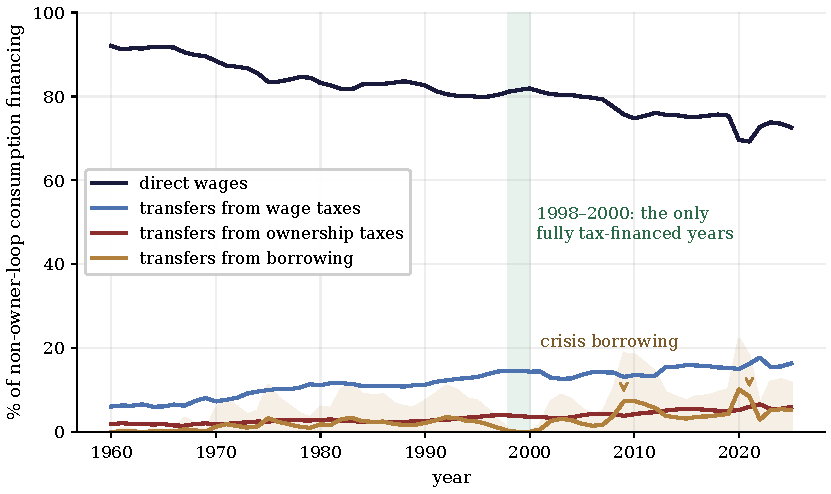
\includegraphics[width=0.88\textwidth]{figures/fig_fourway.pdf}
\caption{Composition of U.S. consumption financing excluding consumption financed
directly from household capital income, in which owners consume their own
returns, 1960--2025. Lines
are medians across the classification-rule grid; the shaded band spans the
deficit-attribution rules. The direct-wage share fell by about twenty
percentage points over sixty years. Transfers grew while about a fifth of
their financing continued to come from taxes on ownership income.
Borrowing financed 19\% of transfers in 2025 and was zero only in
1960, 1963, 1999, and 2000. The allocation follows pro-rata accounting rules; estimating tax
incidence requires a model of behavioral responses. Drawn by code written with Claude (Anthropic).}
\label{fig:8}
\end{figure}

% ---- build part 15_appE.tex (SP/build/parts/15_appE.tex) ----
% =====================================================================================================
% Appendix E. Human-required tasks (app:E). Build part 15, 2026-11-05.
% The authors' Appendix E (main.tex L876-890), verbatim but for two cross-references: the H pointer
% (H is now defined in Assumption 1; design synthesis §1.1, "Let the set H of Assumption 1 have positive
% measure") and the participation pointer. Proposition E.1 keeps its label. Notes: parts/13_17.notes.md.
% =====================================================================================================

% from main.tex L876
\section{Human-required tasks}\label{app:E}

% from main.tex L878, edited: "Let Appendix~\ref{app:A}'s set $H$" -> "Let the set $H$ of
% Assumption~\ref{ass:tasks}" (the H pointer: H is now defined in Assumption 1, design synthesis §1.1; its
% "by capability residue, by verified preference for human hands, or by law" matches Assumption 1, design
% synthesis §3.7, "574, 878")
Let the set $H$ of Assumption~\ref{ass:tasks} have positive measure $|H|$: tasks machines cannot hold --- by capability residue, by verified preference for human hands, or by law --- with $H$-wage $w_H$. Let machines grow unboundedly better at every task outside $H$: $\gamma (x) \to 0$ there, a capability improvement confined to the tasks machines can hold. A worker employed only in $H$ earns a wage determined within the human-required sector. Assume, in a common numeraire, that $w_H$ and $r$ converge to positive finite values, the rental $p_m$ remains bounded, and the machine work outside $H$ has total unit cost tending to zero. Human productivity on $H$ is constant at $\gamma_L>0$. This is a price-path condition: what vanishes is the cost of machine work, $p_m/\gamma _M(x) = p_m\cdot \gamma (x)/\gamma _L(x)$. Aghion, Jones, and Jones (2019) raise the strongest stabilizer this paper faces: Baumol concentration --- expenditure concentrating on the sector whose costs remain positive (Baumol 1967), here the human-required set --- can preserve labor's share indefinitely. Proposition~\ref{prop:E.1} grants the mechanism its theorem and makes its premise explicit.

% from main.tex L880-882
% Review edit (D102): the CES elasticity sigma_H renamed epsilon_H, as in Appendix C
\begin{proposition}[Baumol concentration]\label{prop:E.1}
(i) A good with no additional direct requirement for non-produced inputs whose task list contains $H$ has unit cost tending to $|H|\cdot w_H/\gamma _L$ as $\gamma \to 0$ outside $H$: labor's share of its cost tends to one. (ii) Under CES substitution $\varepsilon _H$ between $H$-content and $H$-light substitutes, the expenditure share of $H$-content tends to 1 if $\varepsilon _H < 1$, to the taste weight if $\varepsilon _H = 1$, and to 0 if $\varepsilon _H > 1$. (iii) On the $\varepsilon _H < 1$ branch with three uses of expenditure (machine-made goods, non-produced services, and human-required services), end-state expenditure splits between the two whose costs remain positive, and labor's aggregate share tends to the human-required share of that split. A persistent human-required sector can sustain a positive wage--rent ratio.
\end{proposition}

% from main.tex L884-886
\begin{proof}
(i) $H$-tasks cost $|H|\cdot w_H/\gamma _L$ whatever machines do; each task outside $H$ costs $p_m\cdot \gamma (x)/\gamma _L(x)$, and the assumed vanishing total cost outside $H$ removes the remainder. (ii) is Appendix~\ref{app:C}'s share display with $q$ read as the relative price of $H$-content: the costlier service's share rises with its relative price iff $\varepsilon _H < 1$, and by (i) that relative price diverges. (iii) An $H$-free good's price vanishes by (i) at $|H| = 0$, so for $\varepsilon _H < 1$ its share vanishes, leaving the split stated in (iii); setting the $H$ taste weight to zero returns the baseline.
\end{proof}

% from main.tex L888
The human-required sector depends on credible provenance and the distribution of demand. A premium for verified human work requires verification and enforceable penalties that make false claims unprofitable. In-person provision makes provenance directly observable, while legal task reservations depend on enforcement. Broadcastable services can concentrate demand on a small number of performers (Rosen 1981), allowing aggregate human-service earnings to persist alongside low earnings for most workers.

% from main.tex L890, edited: "Section~\ref{sec:4}" -> "Section~\ref{sec:participation}" (cross-reference:
% the participation choice is now Section 4.2, with Proposition 3)
% Review edit (D103): n_s, g_s, h_s renamed z_H, z_g, z_h, as in Appendix D.3
% Review edit (R16): "basic living basket" -> "basket", as in D.3
If $H$ employs a minority, most workers receive no income from its protected tasks. Aggregate labor income can therefore persist while the wages of workers outside $H$ fall relative to rents. Their participation depends on support, living costs, and preferences as in Section~\ref{sec:participation}. Human-required services also enter the basket through $\mathbf{z}$. For example, adding $z_H$ hours of care priced at $w_H$ to the two-item basket gives $P_s=pz_g+rz_h+w_Hz_H$ and coverage $\kappa=rT/(NP_s)$. At given rents and other prices, a higher care cost lowers coverage.

% ---- build part 16_appF.tex (SP/build/parts/16_appF.tex) ----
% =====================================================================================================
% Appendix F. The financing and production accounts (app:F). Build part 16, 2026-11-05.
% The authors' Appendix F (main.tex L892-910), verbatim but for the Section 8 pointer and the mapping
% paragraph, which is put on the price coefficients (design synthesis §3.7, "906 (App. F)"). Notes:
% parts/13_17.notes.md.
% =====================================================================================================

% from main.tex L892
\section{The financing and production accounts}\label{app:F}

% from main.tex L894, edited: "Section~\ref{sec:9}" -> "Section~\ref{sec:measurement}" (cross-reference)
Section~\ref{sec:measurement} quotes two shares; this appendix defines and constructs them. The \emph{labor-origin financing share} asks where the purchasing power used for personal consumption originates. The \emph{full-chain human-effort share} asks how much of the purchaser-price value of consumed production resolves into human labor after intermediates are traced recursively.

% from main.tex L896
For 2004--2023 the financing account uses annual BEA source distributions ranked by equivalized disposable income. Spending beyond current disposable income is recorded in an intertemporal bucket; within current-financed spending, tax incidence and allocation across fungible resources are partially identified and reported as bounds. The labor-origin financing share is 69.6\% [59.8--83.1] in 2004 and 65.8\% [52.7--80.1] in 2023; the model-based 2025 extension is 64.2\% [54.1--81.3].

% from main.tex L898
The production account follows the purchaser-price dollar through the production chain. Its BEA benchmark (Samuels and Senel 2026) covers 1997--2023: human effort is 50.1\% of consumed production in 1997 and 47.2\% in 2023. Outside that window, a five-specification product-composition model supplies only a model-based extension, at 66.4\% [61.3--68.6] in 1950 and 46.2\% [45.1--47.4] in 2025. Figure~\ref{fig:7} marks the benchmark-data windows explicitly.

% from main.tex L900
The long extension suggests that the separation is newer than the postwar starting point, but that inference inherits the weaker status of the outer series.

% from main.tex L902-910, edited for the price basis (design synthesis §3.7, row "906 (App. F)":
% w lambda~^T f "on the price basis", reason "cost-based measure"): (a) "\mathbf{A}" -> "\mathbf{A}_\rho" in the cost system, the
% input matrix in prices (Table 1; as Appendix B.2 writes it); (b) ", valued at the user cost," added after
% "The human-effort content of final consumption": the paper's words for the price coefficients (Section 3,
% eq. (4); Section 5 reads \widetilde b_i the same way), since the measured full-chain share is a
% cost-based measure; (c) "\mathsf{T}" -> "\top" (Table 1)
% Review edit (R09): L908: "total human requirements" -> the symbol
\textbf{Mapping back to the model.} The production-content account
corresponds to the common cost system
$\mathbf{p}=\mathbf{A}_\rho\mathbf{p}+\bm{\lambda}w+\mathbf{B}\mathbf{r}$.
The human-effort content of final consumption, valued at the user cost, is
$w\widetilde{\bm{\lambda}}^{\top}\mathbf{f}$, including labor
throughout the supply chain. Recursive automation lowers that content at
given wages and final quantities when $\widetilde{\bm{\lambda}}$ falls; the
observed expenditure share also depends on prices and composition. The
financing-origin account supplies $\varphi_C$ for Appendix~\ref{app:D.5}.

% ---- build part 17_back.tex (SP/build/parts/17_back.tex) ----
% =====================================================================================================
% Back matter before the references. Build part 17, 2026-11-05.
% The data, notation and checks note (main.tex L912-913), with its notation sentences replaced by "Table 1
% lists the notation" (build brief §2; design synthesis §1.1, §3.7), and the declaration on generative AI
% (L915-917), verbatim. The references (L919 onward) are another part's. Notes: parts/13_17.notes.md.
% =====================================================================================================

% from main.tex L912
\bigskip\par\noindent\rule{0.35\linewidth}{0.4pt}\par\smallskip
% from main.tex L913, edited: (a) the two notation sentences after "\textbf{Notation.}" ("In
% Appendices~\ref{app:A.4} and~\ref{app:B} and Figure~\ref{fig:3}, the scalars ... and $s$ denotes the
% reservation wage." and "Direct requirements of the non-produced input are $b_i$, total requirements are
% $\widetilde{b}_i$, and $P_s$ is the cost of the basic living basket.") -> "Table~\ref{tab:notation} lists
% the notation." (build brief §2; design synthesis §3.7, "913"); (b) "solves Appendix~\ref{app:B}'s
% equilibrium" -> "solves Section~\ref{sec:example}'s equilibrium" (cross-reference: the numerical
% instance is now Section 7)
\noindent{\footnotesize\singlespacing \textbf{Data and computation.} All U.S. figures are gross annual flows computed from BEA national accounts (annual NIPA series retrieved via FRED, 2026 vintage), with Federal Reserve Z.1 balance-sheet lines, BEA fixed-assets stocks, and the CPI for the coverage ratio. Financing splits 1960--2025, coverage ratio 1953--2025, deflator fork 1964--2024 on complete calendar years, with the food comparison from the CPI food index (FRED CPIUFDNS) over the same window. Reported values are medians with min--max bands across a rule grid. Flows are gross. The financing series uses annual BEA source profiles ranked by equivalized disposable income in 2004--2023 with partial-identification bounds and weaker outer extensions. The production series uses the BEA full-chain benchmark of Samuels and Senel (2026) in 1997--2023 and a five-specification NIPA product-composition extension outside that window. \textbf{Notation.} Table~\ref{tab:notation} lists the notation.\par \textbf{Numerical checks.} The accompanying \texttt{check\_cost\_system.py} compares network prices with independently truncated production rounds, checks factor-income cancellation and feasible-method bounds, and verifies participation choices directly from utility. The companion \texttt{check\_interior.py} checks task costs and income accounting, solves Section~\ref{sec:example}'s equilibrium, and compares its output against an independently specified linear production program with 2,048 task cells. These checks accompany the analytical proofs.\par}

% from main.tex L915-917
\section*{Declaration of generative AI and AI-assisted technologies in the manuscript preparation process}

During the preparation of this work the authors used Claude (Anthropic) and ChatGPT (OpenAI) to draft parts of the formalization, proofs, computations, figures, and initial prose, under the authors' direction. The theory and its central claims are the authors'. After using these tools, the authors reviewed and edited the content as needed and take full responsibility for the content of the published article. All data were pulled live from public sources; the code and data are public.

% ---- references (build step: assembly) ----
% from main.tex L919-981, edited: the entries not cited in the assembled text are removed, and the six new
% entries of build brief §5 are added in alphabetical order (marked "% NEW (build brief §5)"). Every
% remaining entry is verbatim. SP/build/ASSEMBLY.md lists the removed and the added entries.
\section*{References}

{\small\singlespacing
% assembly (typesetting only, no text change): \sloppy, local to this group. Without it the new Trammell
% and Korinek entry (build brief §5) runs 29.5pt into the margin at its DOI, which can break only after
% "10.1146/". It changes that entry alone (two loose lines); every other entry breaks as before.
\sloppy
\refentry{Acemoglu, D., and P. Restrepo (2018). ``The Race between Man and Machine: Implications of Technology for Growth, Factor Shares, and Employment.'' \emph{American Economic Review} 108(6): 1488--1542. \url{https://doi.org/10.1257/aer.20160696}.}
\refentry{Acemoglu, D., and P. Restrepo (2026). ``Automation and Rent Dissipation: Implications for Wages, Inequality, and Productivity.'' \emph{The Quarterly Journal of Economics} 141(2): 1521--1579. \url{https://doi.org/10.1093/qje/qjag006}.}
\refentry{Aghion, P., B. F. Jones, and C. I. Jones (2019). ``Artificial Intelligence and Economic Growth.'' In A. Agrawal, J. Gans, and A. Goldfarb (eds.), \emph{The Economics of Artificial Intelligence: An Agenda}, University of Chicago Press, pp. 237--282. \url{https://doi.org/10.7208/chicago/9780226613475.003.0009}.}
\refentry{Arnott, R. J., and J. E. Stiglitz (1979). ``Aggregate Land Rents, Expenditure on Public Goods, and Optimal City Size.'' \emph{The Quarterly Journal of Economics} 93(4): 471--500. \url{https://doi.org/10.2307/1884466}.}
\refentry{Arrow, K. J. (1951). ``An Extension of the Basic Theorems of Classical Welfare Economics.'' In \emph{Proceedings of the Second Berkeley Symposium on Mathematical Statistics and Probability}, University of California Press, pp. 507--532. \url{https://doi.org/10.1525/9780520411586-038}.}
\refentry{Autor, D., and D. Dorn (2013). ``The Growth of Low-Skill Service Jobs and the Polarization of the US Labor Market.'' \emph{American Economic Review} 103(5): 1553--1597. \url{https://doi.org/10.1257/aer.103.5.1553}.}
\refentry{Autor, D., F. Levy, and R. J. Murnane (2003). ``The Skill Content of Recent Technological Change: An Empirical Exploration.'' \emph{The Quarterly Journal of Economics} 118(4): 1279--1333. \url{https://doi.org/10.1162/003355303322552801}.}
\refentry{Baumol, W. J. (1967). ``Macroeconomics of Unbalanced Growth: The Anatomy of Urban Crisis.'' \emph{American Economic Review} 57(3): 415--426.}
\refentry{Bouscasse, P., E. Nakamura, and J. Steinsson (2025). ``When Did Growth Begin? New Estimates of Productivity Growth in England from 1250 to 1870.'' \emph{The Quarterly Journal of Economics} 140(2): 835--888. \url{https://doi.org/10.1093/qje/qjae046}.}
\refentry{Card, D., A. R. Cardoso, J. Heining, and P. Kline (2018). ``Firms and Labor Market Inequality: Evidence and Some Theory.'' \emph{Journal of Labor Economics} 36(S1): S13--S70. \url{https://doi.org/10.1086/694153}.}
\refentry{Caselli, F., and A. Manning (2019). ``Robot Arithmetic: New Technology and Wages.'' \emph{American Economic Review: Insights} 1(1): 1--12. \url{https://doi.org/10.1257/aeri.20170036}.}
\refentry{Diamond, P., and J. Mirrlees (1971). ``Optimal Taxation and Public Production I: Production Efficiency.'' \emph{American Economic Review} 61(1): 8--27.}
\refentry{George, H. (1879). \emph{Progress and Poverty.}}
\refentry{Grossman, G. M., and E. Rossi-Hansberg (2008). ``Trading Tasks: A Simple Theory of Offshoring.'' \emph{American Economic Review} 98(5): 1978--1997. \url{https://doi.org/10.1257/aer.98.5.1978}.}
\refentry{Gruber, J. (1997). ``The Incidence of Payroll Taxation: Evidence from Chile.'' \emph{Journal of Labor Economics} 15(3, Part 2): S72--S101. \url{https://doi.org/10.1086/209877}.}
\refentry{Hoynes, H., and J. Rothstein (2019). ``Universal Basic Income in the United States and Advanced Countries.'' \emph{Annual Review of Economics} 11: 929--958. \url{https://doi.org/10.1146/annurev-economics-080218-030237}.}
\refentry{Jones, D., and I. Marinescu (2022). ``The Labor Market Impacts of Universal and Permanent Cash Transfers: Evidence from the Alaska Permanent Fund.'' \emph{American Economic Journal: Economic Policy} 14(2): 315--340. \url{https://doi.org/10.1257/pol.20190299}.}
\refentry{Karabarbounis, L., and B. Neiman (2014). ``The Global Decline of the Labor Share.'' \emph{The Quarterly Journal of Economics} 129(1): 61--103. \url{https://doi.org/10.1093/qje/qjt032}.}
% NEW (build brief §5)
\refentry{Keynes, J. M. (1930). ``Economic Possibilities for our Grandchildren.'' \emph{The Nation and Athenaeum}, 11 and 18 October 1930. Reprinted in \emph{Essays in Persuasion}, Macmillan, 1931, pp. 358--373.}
\refentry{Keynes, J. M. (1936). \emph{The General Theory of Employment, Interest and Money.}}
\refentry{Knoll, K., M. Schularick, and T. Steger (2017). ``No Price Like Home: Global House Prices, 1870--2012.'' \emph{American Economic Review} 107(2): 331--353. \url{https://doi.org/10.1257/aer.20150501}.}
% NEW (build brief §5)
\refentry{Korinek, A., and M. Juelfs (2022). ``Preparing for the (Non-Existent?) Future of Work.'' NBER Working Paper 30172. \url{https://doi.org/10.3386/w30172}.}
% NEW (build brief §5)
\refentry{Korinek, A., and L. Lockwood (2026). ``Public Finance in the Age of AI: A Primer.'' NBER Working Paper 34873. \url{https://doi.org/10.3386/w34873}.}
\refentry{Korinek, A., and J. E. Stiglitz (2019). ``Artificial Intelligence and Its Implications for Income Distribution and Unemployment.'' In A. Agrawal, J. Gans, and A. Goldfarb (eds.), \emph{The Economics of Artificial Intelligence: An Agenda}, University of Chicago Press, pp. 349--390. \url{https://doi.org/10.7208/chicago/9780226613475.003.0014}.}
\refentry{Korinek, A., and D. Suh (2024). ``Scenarios for the Transition to AGI.'' NBER Working Paper 32255. \url{https://doi.org/10.3386/w32255}.}
\refentry{Kugler, A., and M. Kugler (2009). ``Labor Market Effects of Payroll Taxes in Developing Countries: Evidence from Colombia.'' \emph{Economic Development and Cultural Change} 57(2): 335--358. \url{https://doi.org/10.1086/592839}.}
\refentry{Leontief, W. W. (1936). ``Quantitative Input and Output Relations in the Economic Systems of the United States.'' \emph{The Review of Economics and Statistics} 18(3): 105--125. \url{https://doi.org/10.2307/1927837}.}
% NEW (build brief §5)
\refentry{Leontief, W. W. (1983). ``National Perspective: The Definition of Problems and Opportunities.'' In \emph{The Long-Term Impact of Technology on Employment and Unemployment: A National Academy of Engineering Symposium, June 30, 1983}, National Academy Press, pp. 3--7. \url{https://doi.org/10.17226/19470}.}
\refentry{Lewis, W. A. (1954). ``Economic Development with Unlimited Supplies of Labour.'' \emph{The Manchester School} 22(2): 139--191. \url{https://doi.org/10.1111/j.1467-9957.1954.tb00021.x}.}
\refentry{Marx, K. (1867). \emph{Capital: A Critique of Political Economy.} Vol.~1.}
\refentry{Mas, A., and A. Pallais (2019). ``Labor Supply and the Value of Non-Work Time: Experimental Estimates from the Field.'' \emph{American Economic Review: Insights} 1(1): 111--126. \url{https://doi.org/10.1257/aeri.20180070}.}
\refentry{Polanyi, K. (1944). \emph{The Great Transformation.}}
% NEW (build brief §5)
\refentry{Restrepo, P. (2025). ``We Won't be Missed: Work and Growth in the AGI World.'' NBER Working Paper 34423. \url{https://doi.org/10.3386/w34423}.}
\refentry{Rognlie, M. (2015). ``Deciphering the Fall and Rise in the Net Capital Share: Accumulation or Scarcity?'' \emph{Brookings Papers on Economic Activity} 2015(1): 1--69. \url{https://doi.org/10.1353/eca.2016.0002}.}
\refentry{Romer, P. M. (1990). ``Endogenous Technological Change.'' \emph{Journal of Political Economy} 98(5, Part 2): S71--S102. \url{https://doi.org/10.1086/261725}.}
\refentry{Rosen, S. (1981). ``The Economics of Superstars.'' \emph{American Economic Review} 71(5): 845--858.}
\refentry{Saez, E., B. Schoefer, and D. Seim (2019). ``Payroll Taxes, Firm Behavior, and Rent Sharing: Evidence from a Young Workers' Tax Cut in Sweden.'' \emph{American Economic Review} 109(5): 1717--1763. \url{https://doi.org/10.1257/aer.20171937}.}
\refentry{Samuels, J. D., and G. Senel (2026). ``A Value Chain Approach to Measuring the U.S. Production Structure.'' BEA Working Paper WP2026-01, U.S. Bureau of Economic Analysis. \url{https://doi.org/10.66137/IVQT8545}.}
\refentry{Shapiro, C., and J. E. Stiglitz (1984). ``Equilibrium Unemployment as a Worker Discipline Device.'' \emph{American Economic Review} 74(3): 433--444.}
\refentry{Sraffa, P. (1960). \emph{Production of Commodities by Means of Commodities.} Cambridge University Press.}
% NEW (build brief §5)
\refentry{Trammell, P., and A. Korinek (2026). ``Economic Growth under Transformative AI.'' \emph{Annual Review of Economics} 18: 589--611. \url{https://doi.org/10.1146/annurev-economics-051624-061002}.}
\refentry{Zeira, J. (1998). ``Workers, Machines, and Economic Growth.'' \emph{The Quarterly Journal of Economics} 113(4): 1091--1117. \url{https://doi.org/10.1162/003355398555847}.}\par
}

% from main.tex L983
\end{document}
